% Editable teaching source. Compile with XeLaTeX (twice) or Tectonic.
\ifdefined\TeachingHandout
  \documentclass[handout,aspectratio=169,10pt]{beamer}
\else
  \documentclass[aspectratio=169,10pt]{beamer}
\fi
\usepackage[T1]{fontenc}
\usepackage{lmodern}
\usepackage{amsmath,amssymb,mathtools,booktabs,array,tabularx,graphicx,listings,tikz}
\usepackage{pgfplots}
\usetikzlibrary{arrows.meta,positioning,calc,shapes.geometric,fit,decorations.pathreplacing,backgrounds}
\pgfplotsset{compat=1.18}
\definecolor{navy}{HTML}{173F37}
\definecolor{teal}{HTML}{08734F}
\definecolor{amber}{HTML}{A66610}
\definecolor{red}{HTML}{B83136}
\definecolor{slate}{HTML}{52635E}
\definecolor{pale}{HTML}{EDF5F0}
\definecolor{blue}{HTML}{245F9B}
\setbeamercolor{normal text}{fg=black!90,bg=white}
\setbeamercolor{structure}{fg=teal}
\setbeamercolor{frametitle}{fg=navy,bg=white}
\setbeamercolor{alerted text}{fg=red}
\setbeamercolor{block title}{fg=teal,bg=pale}
\setbeamercolor{block body}{fg=black!90,bg=pale}
\setbeamerfont{frametitle}{size=\large,series=\bfseries}
\setbeamerfont{block title}{size=\normalsize,series=\bfseries}
\setbeamerfont{block body}{size=\normalsize}
\setbeamersize{text margin left=.55cm,text margin right=.55cm}
\setbeamertemplate{navigation symbols}{}
\setbeamertemplate{itemize items}[circle]
\setbeamertemplate{blocks}[default]
\setbeamercovered{transparent=8}
\newcommand{\TeachingSource}{}
\newcommand{\TeachingBridge}{}
\newcommand{\Source}[1]{\gdef\TeachingSource{#1}}
\newcommand{\Bridge}[1]{\gdef\TeachingBridge{#1}\transfade[duration=.18]}
\setbeamertemplate{headline}{\begin{beamercolorbox}[wd=\paperwidth,ht=.36cm,dp=.08cm,leftskip=.55cm]{normal text}\scriptsize\color{teal}\insertsectionhead\strut\end{beamercolorbox}}
\setbeamertemplate{frametitle}{\vspace{.02cm}\insertframetitle\par\vspace{.1cm}\textcolor{teal}{\rule{\linewidth}{.7pt}}\vspace{-.12cm}}
\setbeamertemplate{footline}{%
 \begin{beamercolorbox}[wd=\paperwidth,ht=.88cm,dp=.08cm,leftskip=.55cm,rightskip=.55cm]{normal text}
 \begin{minipage}[b][.82cm][t]{14.9cm}
 \parbox[t][.34cm][t]{\linewidth}{\fontsize{6.3}{7.3}\selectfont\color{slate}\TeachingSource\strut}
 \par\vspace{.02cm}\textcolor{teal!35}{\rule{\linewidth}{.3pt}}\par\vspace{-.04cm}
 {\fontsize{7}{8}\selectfont\color{navy}\textbf{Next:} \TeachingBridge\hfill\insertframenumber/\inserttotalframenumber\strut\par}
 \end{minipage}\end{beamercolorbox}}
\newcommand{\Idea}[2]{\begin{block}{#1}#2\end{block}}
\newcommand{\Question}[1]{\par\smallskip\textcolor{teal}{\textbf{Predict:}} #1\par}
\newcommand{\Answer}[1]{\uncover<2->{\par\smallskip\textcolor{teal}{\textbf{Explanation:}} #1\par}}
\newcommand{\Checkpoint}[2]{\par{\small\color{teal}\textbf{Notebook #1}\quad #2}\par\smallskip}
\newcommand{\Code}[1]{\lstinputlisting[style=python]{snippets/#1}}
\newcommand{\yesmark}{\textcolor{teal}{\checkmark}}
\newcommand{\nomark}{\textcolor{slate}{---}}
\newcommand{\partmark}{\textcolor{amber}{\ensuremath{\triangle}}}
\lstdefinestyle{python}{language=Python,basicstyle=\ttfamily\fontsize{7.2}{8.8}\selectfont,keywordstyle=\color{teal}\bfseries,commentstyle=\color{slate},stringstyle=\color{amber},backgroundcolor=\color{pale},frame=none,columns=fullflexible,keepspaces=true,showstringspaces=false,breaklines=true,tabsize=4,xleftmargin=.12cm,xrightmargin=.12cm,aboveskip=.12cm,belowskip=.12cm}
\tikzset{box/.style={draw=teal,fill=pale,rounded corners=2pt,align=center,font=\small,inner sep=5pt},arrow/.style={-{Stealth[length=2mm]},thick,draw=teal},every picture/.style={line width=.7pt}}
\setlength{\parskip}{0pt}
\setlength{\tabcolsep}{4pt}
\renewcommand{\arraystretch}{1.15}
\hypersetup{colorlinks=true,linkcolor=teal,urlcolor=teal,pdftitle={Agentic AI for Grid Operators: a worked teaching sequence},pdfsubject={Native LaTeX teaching slides, notebook experiments and evidence}}
\setbeameroption{hide notes}

\begin{document}
\section{Foundations: from an alarm to a checked action}
% Native teaching edition: 41 frames, F01--F40 plus F05A.
% The opening arithmetic is illustrative, not a feeder model.

\begin{frame}[t]{An alarm is a question: what can the operator change?}
\label{f:F01}
\begin{columns}[T,onlytextwidth]
\column{.49\textwidth}
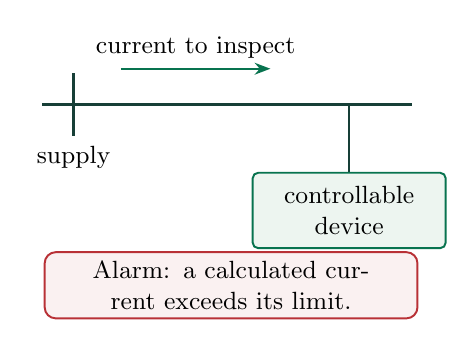
\begin{tikzpicture}[x=1cm,y=1cm]
\draw[very thick,navy] (0,1.8)--(4.7,1.8);
\draw[thick,navy] (.4,1.4)--(.4,2.2);
\node[below,font=\small] at (.4,1.4) {supply};
\draw[thick,navy] (3.9,1.8)--(3.9,.9);
\node[box,text width=2.1cm] at (3.9,.45) {controllable\\device};
\draw[arrow] (1,2.25)--node[above,font=\small] {current to inspect}(2.9,2.25);
\node[draw=red,fill=red!7,rounded corners,align=center,text width=4.5cm,font=\small] at (2.4,-.5) {Alarm: a calculated current exceeds its limit.};
\end{tikzpicture}\par
\column{.47\textwidth}
\Idea{A physical question}{Which permitted command reduces the loading enough, and what evidence supports it?}
\uncover<2->{\Idea{An operator needs}{The candidate, the calculated consequence, the limit, and the model used.}}
\end{columns}
\medskip
We start with one small worked decision. Its arithmetic is invented so that every step can be checked by hand; the feeder models come later.
\Source{Teaching schematic; \href{../Graph_Workflow_Lab.ipynb}{Graph lab G0--G5} declares the toy scope.}
\Bridge{Can we calculate the alarm with three numbers?}
\note{Begin by asking what an operator would need before changing a command. Do not begin with a definition of an agent. The line drawing is a physical motivation, not an electrical model of the Greensboro feeder. Its purpose is to separate a proposed command from the consequence that must be checked. The upcoming arithmetic is deliberately invented and dimensionless so everyone can reproduce it without a simulator. Later, actual feeder tools will replace that arithmetic while the evidence discipline remains. Reveal the operator requirements only after one response from the room. The expected interpretation is that an alarm identifies a problem, but it does not uniquely identify an acceptable action. Next, turn the question into a fully specified calculation.}
\end{frame}

\begin{frame}[t]{Work the alarm: the proposed command gives too much current}
\label{f:F02}
\[
 \underbrace{i}_{\text{toy current}}
 =0.4+0.8\underbrace{u}_{\text{command}},
 \qquad \underbrace{L}_{\text{toy limit}}=0.80.
\]
\begin{columns}[T,onlytextwidth]
\column{.47\textwidth}
\textbf{Proposed input:} set the dimensionless command to \(u=0.75\).
\uncover<2->{\[
i=0.4+0.8(0.75)=1.00.
\]}
\column{.49\textwidth}
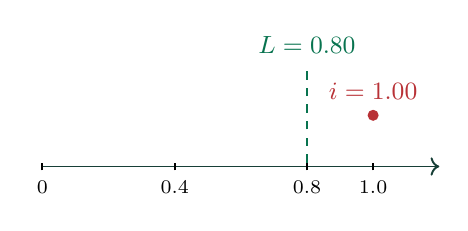
\begin{tikzpicture}[x=4.2cm,y=1cm]
\draw[->,navy] (0,0)--(1.2,0);
\foreach \x/\s in {0/0,.4/0.4,.8/0.8,1/1.0}
{\draw (\x,-.05)--(\x,.05);\node[below,font=\scriptsize] at (\x,-.06) {\s};}
\draw[dashed,teal] (.8,.05)--(.8,1.3);
\node[above,font=\small,teal] at (.8,1.3) {\(L=0.80\)};
\uncover<2->{\fill[red] (1,.65) circle (2pt);
\node[above,font=\small,red] at (1,.72) {\(i=1.00\)};}
\end{tikzpicture}\par
\uncover<3->{\par\smallskip\textbf{Verdict:} \(1.00>0.80\), so the candidate fails. The excess is \(i-L=0.20\).}
\end{columns}
\medskip
Both \(i\) and \(L\) are normalized illustrative quantities, not amperes. A correct calculation can still return an unacceptable operating point.
\Source{Exact response and comparison used in \href{../Graph_Workflow_Lab.ipynb}{G2 and G4}.}
\Bridge{What does one permitted repair change?}
\note{Read each symbol aloud before substituting the numbers. The command u is dimensionless, the calculated current i is a normalized illustrative quantity, and L is its limit in the same normalization. The constants define an invented response law. Multiplication gives 0.60, so adding the offset gives 1.00. The comparison with 0.80 is a separate step from that arithmetic. Ask whether the calculation itself failed; it did not. It correctly identified an inadmissible candidate. Reveal the point on the number line, then the verdict. The expected interpretation is that simulation and verification answer different questions. A converged or correctly executed calculation is not automatically an acceptable result. Next, change the command using an explicit repair rule.}
\end{frame}

\begin{frame}[t]{Repair the command, then recalculate its consequence}
\label{f:F03}
\[
u_{\mathrm{new}}=\max(0,u_{\mathrm{old}}-0.25)
=\max(0,0.75-0.25)=0.50.
\]
\begin{center}
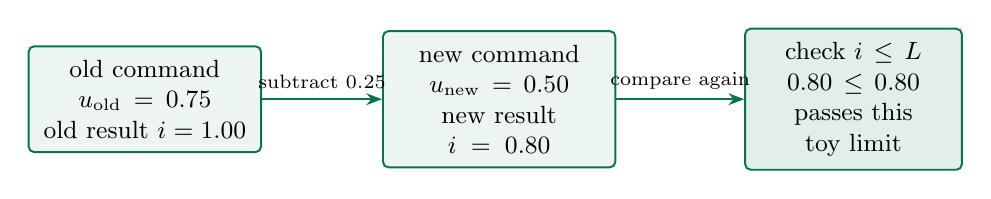
\begin{tikzpicture}
\node[box,text width=2.6cm] (old) at (0,0) {old command\\\(u_{\mathrm{old}}=0.75\)\\old result \(i=1.00\)};
\node[box,text width=2.6cm] (new) at (4.5,0) {new command\\\(u_{\mathrm{new}}=0.50\)\\new result \(i=0.80\)};
\node[box,text width=2.4cm,fill=teal!12] (ok) at (9,0) {check \(i\leq L\)\\\(0.80\leq0.80\)\\passes this toy limit};
\draw[arrow] (old)--node[above,font=\scriptsize] {subtract \(0.25\)}(new);
\draw[arrow] (new)--node[above,font=\scriptsize] {compare again}(ok);
\end{tikzpicture}\par
\end{center}
\(u_{\mathrm{old}}\) and \(u_{\mathrm{new}}\) are the commands before and after repair. The lower bound of zero prevents a negative command.
\medskip
\uncover<3->{The old current belongs to the old command. Reusing it would give the wrong decision about the repaired command.}
\Source{Repair and simulation functions: \href{../Graph_Workflow_Lab.ipynb}{G2}.}
\Bridge{Which pieces of work did we just perform?}
\note{Work the subtraction first and ask the class to calculate the new current. The repair produces 0.50, and the response law produces 0.80. Equality passes because the declared rule is less than or equal to the limit. The zero in the maximum is a bound on the command, not an extra simulation result. The important process lesson is that changing the command invalidates the previous current as evidence for that new command. A record may preserve the old value as history, but a new verification must use the new calculation. Reveal the last box only after the audience predicts the result. The expected interpretation is a complete candidate, calculation, and comparison sequence. Next, name those responsibilities without yet introducing software terminology.}
\end{frame}

\begin{frame}[t]{The operator's calculation already has a workflow}
\label{f:F04}
\begin{center}
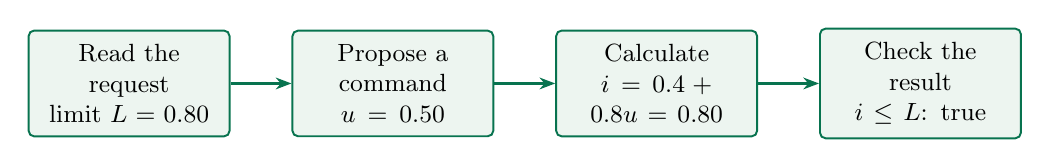
\begin{tikzpicture}
\node[box,text width=2.2cm] (a) at (0,0) {Read the request\\limit \(L=0.80\)};
\node[box,text width=2.2cm] (b) at (3.35,0) {Propose a command\\\(u=0.50\)};
\node[box,text width=2.2cm] (c) at (6.7,0) {Calculate\\\(i=0.4+0.8u=0.80\)};
\node[box,text width=2.2cm] (d) at (10.05,0) {Check the result\\\(i\leq L\): true};
\draw[arrow] (a)--(b);\draw[arrow] (b)--(c);\draw[arrow] (c)--(d);
\end{tikzpicture}\par
\end{center}
\Idea{A dependency}{We cannot check the consequence of this command until its calculation returns.}
\uncover<2->{\Idea{A record}{Keep the request, command, result, limit, and verdict together.}}
\uncover<3->{\Idea{A next decision}{A pass permits review; a failure asks for repair or a hold.}}
\Source{Tutorial decomposition; executable functions in \href{../Graph_Workflow_Lab.ipynb}{G1--G3}.}
\Bridge{What should the operator actually see at review?}
\note{The four boxes are now meaningful because each contains a number the audience has already calculated. Read the arrows as requirements, not as electrical lines. The current must exist before the comparison can be performed, and the command must exist before its consequence can be calculated. These dependencies explain why a workflow is useful without relying on a vague automation claim. Ask what would be lost if only the final word pass were stored. The audience should identify the command, limit, or model assumptions that make that word interpretable. A later language model can help select permitted work, but it does not eliminate these dependencies. The expected interpretation is that the workflow organizes familiar engineering responsibilities. Next, put the results into a concrete review record.}
\end{frame}

\begin{frame}[t]{A reviewable recommendation is more than a pass label}
\label{f:F05}
\begin{columns}[T,onlytextwidth]
\column{.53\textwidth}
\begin{tabular}{@{}>{\raggedright\arraybackslash}p{3.4cm}>{\raggedright\arraybackslash}p{3.5cm}@{}}
\textbf{Recommendation record} & \textbf{Value}\\\hline
Candidate command & \(u=0.50\)\\
Toy current & \(i=0.80\)\\
Declared limit & \(L=0.80\)\\
Model scope & invented toy equation\\
Review identity & bound to this recommendation
\end{tabular}\par
\column{.43\textwidth}
\Question{Would the same acknowledgment apply after changing \(u\)?}
\Answer{No. A changed recommendation needs its own evidence and matching readback.}
\end{columns}
\medskip
\uncover<3->{The G5 exercise records a simulated acknowledgment. It neither authenticates an operator nor sends a command to equipment.}
\Source{Review payload and identity test: \href{../Graph_Workflow_Lab.ipynb}{G5}; engineering handoff: \href{../Classroom_Labs.ipynb}{L12}.}
\Bridge{Where will these ideas lead during the three-hour tutorial?}
\note{Read the recommendation record as something an operator can challenge. The command says what is proposed, the consequence says what was calculated, and the scope says how far the calculation applies. The identity field ties a response to this recommendation rather than to a vaguely remembered previous one. Ask whether a changed command should inherit the previous acknowledgment. The expected answer is no, even if the numerical difference is small. In the graph lab, the response is scripted inside the notebook and represents a simulated readback. It demonstrates state handling rather than authentication or dispatch. The later engineering packet uses the same distinction between evidence and acknowledgment. Next, place this small example within the full teaching route and its three physical cases.}
\end{frame}

\begin{frame}[t]{Three hours: understand a process, then challenge it in code}
\label{f:F05A}
\small
\begin{tabular}{@{}>{\raggedright\arraybackslash}p{1.5cm}>{\raggedright\arraybackslash}p{6cm}>{\raggedright\arraybackslash}p{4.0cm}@{}}
\textbf{Minutes} & \textbf{Question we will answer} & \textbf{Hands-on checkpoint}\\\hline
0--40 & How do state, tools, and decisions connect? & G0--G5; L0--L1\\
40--80 & Which inverter command meets the limits? & L2--L5; Llama evidence\\
80--90 & Break & Keep the kernels available\\
90--115 & Which permitted restoration choice serves priorities? & L6--L7\\
115--142 & Which measurements can support a response? & L8--L9\\
142--180 & What does the evidence justify for the operator? & L10--L12; capstone
\end{tabular}\par
\medskip
\uncover<2->{Every exercise follows \textbf{predict, run, explain}. A fresh numerical result, an archived actual Llama reply, and a new Llama call have different labels.}
\Source{Executable teaching route: \href{../Graph_Workflow_Lab.ipynb}{graph notebook} and \href{../Classroom_Labs.ipynb}{engineering notebook}.}
\Bridge{Which repeated parts of our calculation are worth automating?}
\note{Use the timetable to set a practical pace. Installation is a prerequisite; the class should not begin installing a large language model during the voltage exercise. Participants need the graph notebook and the classroom notebook, with the working directory set as documented. The first uses transparent arithmetic to expose execution mechanics. The second connects numerical methods, stored learned weights, and explicitly labeled language-model evidence. Preserve the difference between an archived reply and a newly generated reply when discussing latency or reproducibility. The course includes a ten-minute break and time to interpret outputs rather than continuously advance slides. The expected interpretation is a sequence of connected experiments, not a slide lecture followed by unrelated code. Next, examine which repeated responsibilities automation can make explicit.}
\end{frame}

\begin{frame}[t]{Automate the repeated work; keep its evidence visible}
\label{f:F06}
\begin{center}
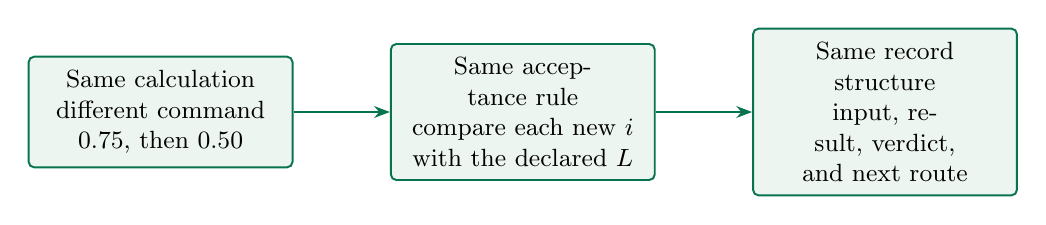
\begin{tikzpicture}
\node[box,text width=3cm] (a) at (0,0) {Same calculation\\different command\\\(0.75\), then \(0.50\)};
\node[box,text width=3cm] (b) at (4.6,0) {Same acceptance rule\\compare each new \(i\)\\with the declared \(L\)};
\node[box,text width=3cm] (c) at (9.2,0) {Same record structure\\input, result, verdict,\\and next route};
\draw[arrow] (a)--(b);\draw[arrow] (b)--(c);
\end{tikzpicture}\par
\end{center}
\uncover<2->{A conventional program can perform all three responsibilities. An agentic design must earn its value through useful choices, clearer evidence, or adaptable task handling.}
\medskip
\uncover<3->{We will compare numerical outcome, recorded checks, and elapsed time separately. More model calls do not by themselves establish an advantage.}
\Source{Matched evaluation: \href{https://arxiv.org/html/2606.18789v1}{PowerAgentBench-SS, 2026 preprint}; tutorial baseline: \href{../Graph_Workflow_Lab.ipynb}{G4}.}
\Bridge{What do tool, agent, and orchestrator mean for this exact calculation?}
\note{Begin with work the audience recognizes: apply the response law again, compare with a limit again, and record what happened. A fixed supervisor can automate all of it. This is important because the tutorial should not assign ordinary software benefits exclusively to language models. The agentic contribution must be identified and tested, such as selecting useful follow-up work from a bounded catalog or helping assemble an interpretable response. These contributions can be helpful while leaving the numerical action unchanged, and they can introduce latency. The graph baseline later makes this distinction concrete by matching all three toy outcomes. The expected interpretation is a testable motivation for the architecture rather than an assumption of superiority. Next, name the components by the jobs they actually perform.}
\end{frame}

\begin{frame}[t]{Three names for three jobs we have already seen}
\label{f:F07}
\begin{center}
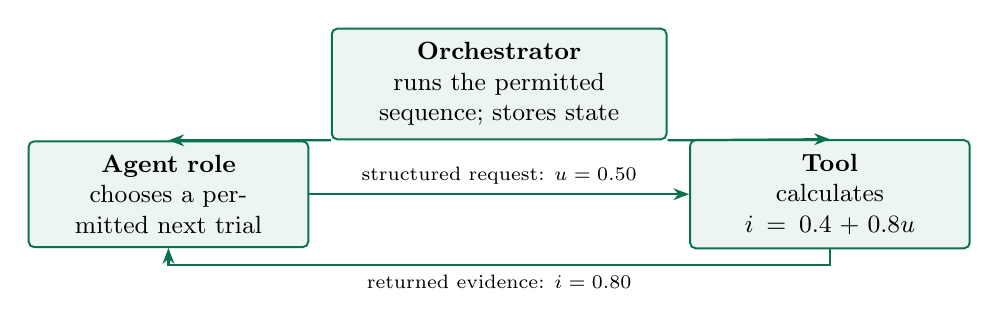
\begin{tikzpicture}
\node[box,text width=3.9cm] (o) at (4.2,1.4) {\textbf{Orchestrator}\\runs the permitted sequence; stores state};
\node[box,text width=3.2cm] (a) at (0,0) {\textbf{Agent role}\\chooses a permitted next trial};
\node[box,text width=3.2cm] (t) at (8.4,0) {\textbf{Tool}\\calculates \(i=0.4+0.8u\)};
\draw[arrow] (o.south west)--(a.north);
\draw[arrow] (o.south east)--(t.north);
\draw[arrow] (a)--node[above,font=\scriptsize] {structured request: \(u=0.50\)}(t);
\draw[arrow] (t.south)--(8.4,-.9)--node[below,font=\scriptsize] {returned evidence: \(i=0.80\)}(0,-.9)--(a.south);
\end{tikzpicture}\par
\end{center}
A role is a responsibility, not necessarily a separate model. A numerical node can operate without an LLM; several roles can use the same Llama backbone.
\uncover<2->{The graph lab uses deterministic choices. The engineering workflow later adds actual bounded Llama responses.}
\Source{Role-based systems: \href{https://arxiv.org/abs/2308.08155}{AutoGen}; tutorial separation: \href{../src/proposal_workflow.py}{workflow implementation}.}
\Bridge{Where can a language model help without replacing the calculation?}
\note{The diagram deliberately places the orchestrator above the interaction instead of after the tool in a false linear pipeline. Point to the request and returned evidence. The tool performs a specific calculation. The agent role chooses an allowed operation using the current context. The orchestrator makes the sequence and state management explicit. These responsibilities can be implemented in several ways, and their names do not imply independent intelligence or independent errors. The toy's choice policy is ordinary Python, so it does not become a language-model experiment when drawn as a graph. Actual Llama calls appear in the engineering records later. The expected interpretation is a clear division of responsibility. Next, show a bounded language-model decision and the numerical work that must follow it.}
\end{frame}

\begin{frame}[t]{Llama can choose follow-up work; the tool supplies the numbers}
\label{f:F08}
\begin{columns}[T,onlytextwidth]
\column{.48\textwidth}
\Idea{Illustrative language interface}{This candidate exceeds its limit. Choose an allowed repair or request a hold.}
\begin{tabular}{@{}ll@{}}
Allowed operation & Meaning\\\hline
\texttt{REPAIR} & try the declared repair rule\\
\texttt{HOLD} & stop and report the issue
\end{tabular}\par
\column{.48\textwidth}
\uncover<2->{\Idea{What the tool still does}{Calculate the repaired consequence and compare it with the unchanged limit.}}
\uncover<3->{\Idea{What we inspect}{The chosen operation, returned result, verdict, and concise public explanation.}}
\end{columns}
\medskip
\textbf{This is an interface illustration, not a captured model reply.} The toy uses fixed routing; later voltage examples show actual Llama outputs and latency.
\Source{Observe--act feedback: \href{https://arxiv.org/abs/2210.03629}{ReAct}; actual replies: \href{../Classroom_Labs.ipynb}{L3, L10, L11}.}
\Bridge{How does this fit all five stages proposed for the grid workflow?}
\note{Make the evidence label explicit before discussing the example. The prompt and two-operation catalog illustrate a design; they are not an actual model response and are not executed by the toy. The later engineering examples use a different declared operation catalog and contain real archived calls. The language model can help interpret a request and select bounded follow-up work. It cannot make the repaired command acceptable merely by describing it favorably. Numerical evaluation and an unchanged acceptance rule remain necessary. Public explanations can be compared with returned evidence without requesting hidden private reasoning. The expected interpretation is a constrained decision interface with inspectable inputs and outputs. Next, connect that interface to the proposal's complete sequence of responsibilities.}
\end{frame}

\begin{frame}[t]{All five proposed stages have a concrete return value}
\label{f:F09}
\begin{center}
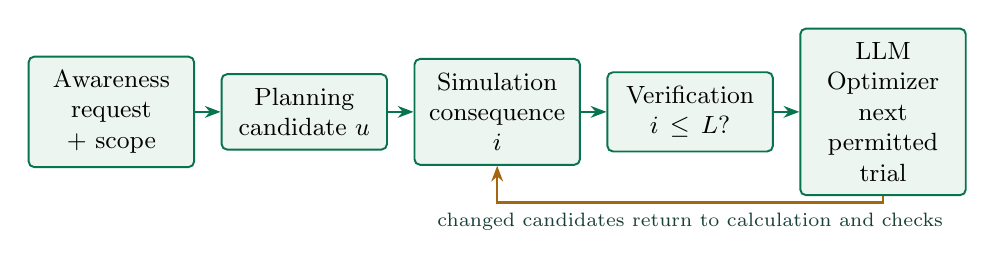
\begin{tikzpicture}
\node[box,text width=1.75cm] (a) at (0,0) {Awareness\\request + scope};
\node[box,text width=1.75cm] (p) at (2.45,0) {Planning\\candidate \(u\)};
\node[box,text width=1.75cm] (s) at (4.9,0) {Simulation\\consequence \(i\)};
\node[box,text width=1.75cm] (v) at (7.35,0) {Verification\\\(i\leq L\)?};
\node[box,text width=1.75cm] (o) at (9.8,0) {LLM Optimizer\\next permitted trial};
\draw[arrow] (a)--(p);\draw[arrow] (p)--(s);\draw[arrow] (s)--(v);\draw[arrow] (v)--(o);
\uncover<2->{\draw[arrow,amber] (o.south)--(9.8,-1.15)--node[below,font=\scriptsize,text=navy] {changed candidates return to calculation and checks}(4.9,-1.15)--(s.south);}
\end{tikzpicture}\par
\end{center}
\uncover<3->{\textbf{Human review} receives the selected candidate, its evidence, alternatives, and unresolved assumptions.}
\medskip
Planning uses a suitable numerical method for each case. The LLM Optimizer selects follow-up work; a new choice is a trial, not an already verified action.
\Source{All five stages and recorded events: \href{../results/proposal_complete_workflow.json}{executed tutorial trace}.}
\Bridge{Which numerical method belongs inside each case?}
\note{Carry one candidate through the five boxes and name the returned artifact at every stage. Awareness establishes the request and model scope. Planning returns a candidate. Simulation returns modeled consequences. Verification returns numerical margins and a verdict. The LLM Optimizer chooses permitted follow-up work, and a changed candidate returns to simulation and verification. Human review occurs after this evidence is assembled. The toy variables illustrate the handoff but do not imply that the toy itself contains five LLM calls. The engineering archive later exposes all five actual stage records, including deterministic events. The expected interpretation is a complete process with an explicit return loop, not five independent votes. Next, select algorithms according to the underlying mathematical problem rather than the role name.}
\end{frame}

\begin{frame}[t]{The workflow reuses numerical methods; it does not replace them}
\label{f:F10}
\begin{tabular}{@{}>{\raggedright\arraybackslash}p{2.1cm}>{\raggedright\arraybackslash}p{4.0cm}>{\raggedright\arraybackslash}p{5.3cm}@{}}
\textbf{Case} & \textbf{Numerical work} & \textbf{What the workflow coordinates}\\\hline
Voltage support & MPC planning; SAC continuous-action proposal & Compare candidates, simulate, check, select a bounded trial\\
Restoration & Mixed-integer service allocation & Preserve priorities and feasible connectivity while evaluating options\\
Cyber response & State estimation, residual tests, constrained response & Distinguish suspicious evidence, supported action, and a hold
\end{tabular}\par
\medskip
\uncover<2->{A model-based method predicts behavior with an explicit model. A model-free policy learns an action rule from experience; training may still use a simulator.}
\uncover<3->{Every candidate faces declared checks. A language-model explanation is not a numerical certificate.}
\Source{Methods: \href{../src/classroom_labs.py}{classroom tools}; \href{https://sites.engineering.ucsb.edu/~jbraw/mpc/}{MPC}; \href{https://proceedings.mlr.press/v80/haarnoja18b.html}{SAC}.}
\Bridge{What information must survive every handoff?}
\note{The method should match the decision variables and evidence available in the case. Voltage control uses continuous inverter commands, so MPC and a learned continuous-action actor are natural examples. Restoration includes discrete service decisions and therefore needs a different formulation. The cyber example begins with measurement evidence and state estimation before a constrained response is considered. The framework coordinates these operations and records their results; it does not make one algorithm universally appropriate. Introduce model-based and model-free at this general level before the detailed equations later. A model-free actor can be trained using simulated experience, which is not a contradiction. The expected interpretation is methods inside the workflow. Next, inspect the common state record that prevents information from being lost between these methods.}
\end{frame}

\begin{frame}[t]{State is the record that keeps this decision coherent}
\label{f:F11}
\begin{columns}[T,onlytextwidth]
\column{.47\textwidth}
\textbf{Before the repair}\par\smallskip
\begin{tabular}{@{}ll@{}}
\texttt{command} & \(0.75\)\\
\texttt{current} & \(1.00\)\\
\texttt{limit} & \(0.80\)\\
\texttt{passed} & false\\
\texttt{attempts} & \(0\)
\end{tabular}\par
\column{.47\textwidth}
\uncover<2->{\textbf{After repair and recalculation}\par\smallskip
\begin{tabular}{@{}ll@{}}
\texttt{command} & \(0.50\)\\
\texttt{current} & \(0.80\)\\
\texttt{limit} & \(0.80\)\\
\texttt{passed} & true\\
\texttt{attempts} & \(1\)
\end{tabular}\par}
\end{columns}
\medskip
\(s_t\) denotes the full record before workflow step \(t\). A node reads that record and returns field updates; unchanged fields remain available.
\uncover<3->{The limit remains \(0.80\). Repairing the command does not authorize relaxing its acceptance criterion.}
\Source{Exact fields and updates: \href{../Graph_Workflow_Lab.ipynb}{G1--G2}.}
\Bridge{How can a diagram make the dependencies in this record visible?}
\note{Use the paired tables as a before-and-after comparison. The command and calculated current change, the verdict changes, and the attempt counter increments. The limit does not change. This makes the separation between changing an action and changing the acceptance criterion concrete. State is more useful than an unstructured conversation for this purpose because each relevant field can be located and checked. The symbol s with a subscript t denotes the entire record before a computational step, not the electrical system state alone. Nodes return updates rather than rewriting unrelated fields. Ask which old value may be preserved in history but must not remain the current result. The expected answer is 1.00. Next, use a graph to display which operations need which record fields.}
\end{frame}

\begin{frame}[t]{Two graphs answer different questions}
\label{f:F12}
\begin{columns}[T,onlytextwidth]
\column{.48\textwidth}
\textbf{Workflow graph: what must run first?}
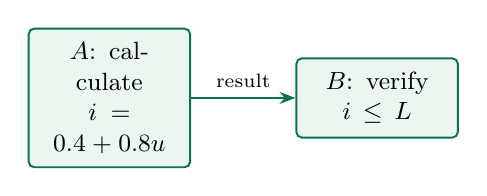
\begin{tikzpicture}
\node[box,text width=1.7cm] (a) at (0,0) {\(A\): calculate\\\(i=0.4+0.8u\)};
\node[box,text width=1.7cm] (b) at (3.4,0) {\(B\): verify\\\(i\leq L\)};
\draw[arrow] (a)--node[above,font=\scriptsize] {result}(b);
\end{tikzpicture}\par
Nodes are operations; \(A\rightarrow B\) means that \(B\) requires a result from \(A\).
\column{.48\textwidth}
\uncover<2->{\textbf{Electrical graph: what is connected?}
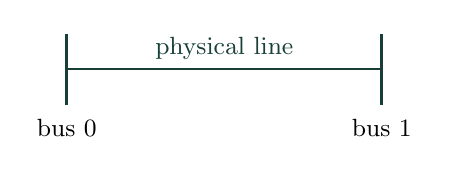
\begin{tikzpicture}
\draw[very thick,navy] (0,-.45)--(0,.45);
\draw[very thick,navy] (4,-.45)--(4,.45);
\draw[thick,navy] (0,0)--node[above,font=\small] {physical line}(4,0);
\node[below,font=\small] at (0,-.5) {bus 0};
\node[below,font=\small] at (4,-.5) {bus 1};
\end{tikzpicture}\par
Nodes are buses; edges are lines or other network connections. Their equations describe electrical behavior.}
\end{columns}
\medskip
\uncover<3->{A tool may solve the electrical graph while the workflow graph controls when that tool runs. The two drawings describe different systems.}
\medskip
\(A,B\): operations; \(s\): shared record; \(r(s)\): a rule returning the next operation label. The earlier \(u,i,L\) remain the toy command, consequence, and limit.
\Source{\href{https://docs.langchain.com/oss/python/langgraph/graph-api}{LangGraph graph API}; \href{https://opendss.epri.com/}{OpenDSS documentation}.}
\Bridge{How can two workflow checks depend on one frozen calculation?}
\note{Read the left and right headings before following either set of edges. The workflow graph describes computations: calculate a result, then use it in verification. The electrical graph describes physical connectivity between buses. A line in the right-hand picture does not specify a software execution order. A power-flow tool can solve equations on that network while the workflow controls when to call the tool and what to do with its output. Ask which drawing would change if an electrical switch opened, and which would change if a review step were added. This distinction will return in restoration, where topology is part of the physical decision. The expected interpretation is two graph meanings with separate node and edge definitions. Next, branch two computations from one frozen input.}
\end{frame}

\begin{frame}[t]{A DAG can branch two checks and join their evidence}
\label{f:F13}
\begin{center}
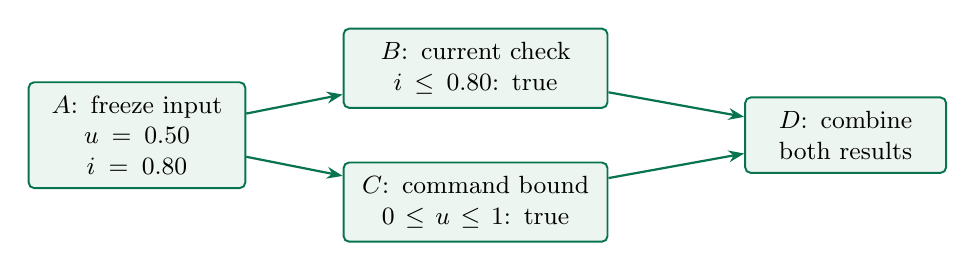
\begin{tikzpicture}
\node[box,text width=2.4cm] (a) at (0,0) {\(A\): freeze input\\\(u=0.50\)\\\(i=0.80\)};
\node[box,text width=3cm] (b) at (4.3,.85) {\(B\): current check\\\(i\leq0.80\): true};
\node[box,text width=3cm] (c) at (4.3,-.85) {\(C\): command bound\\\(0\leq u\leq1\): true};
\node[box,text width=2.2cm] (d) at (9,0) {\(D\): combine\\both results};
\draw[arrow] (a)--(b);\draw[arrow] (a)--(c);\draw[arrow] (b)--(d);\draw[arrow] (c)--(d);
\end{tikzpicture}\par
\end{center}
\(\mathcal G=(N,E)\): \(N=\{A,B,C,D\}\) is the operation set; \(E\) contains the directed dependency arrows.
\medskip
\uncover<2->{\textbf{Directed}: arrows have direction. \textbf{Acyclic}: no directed path returns to its start. This is a DAG.}
\uncover<3->{This teaching example is not the G-lab topology. The join requires both results for the same frozen input.}
\Source{DAG ordering: \href{https://networkx.org/documentation/stable/reference/algorithms/generated/networkx.algorithms.dag.topological_sort.html}{NetworkX}; illustrative checks use the declared toy variables.}
\Bridge{Which execution orders respect every dependency?}
\note{The example now branches only after the input and calculated current have been frozen. One operation checks the current limit, and another checks the declared command range. Both use the same candidate. The final operation combines their results and must wait for both. Define the graph, node set, and edge set directly under the drawing so no symbol is unexplained. A directed acyclic graph has no path that follows arrows back to its starting node. These conceptual checks might be independent, but the picture does not claim that the engineering adapters execute concurrently. It also differs from the cyclic graph in the lab. The expected interpretation is a prerequisite structure with a genuine join. Next, ask the audience to choose valid schedules.}
\end{frame}

\begin{frame}[t]{A valid schedule puts both checks before the join}
\label{f:F14}
\begin{columns}[T,onlytextwidth]
\column{.47\textwidth}
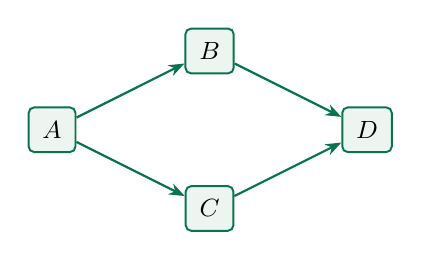
\begin{tikzpicture}
\node[box] (a) at (0,0) {\(A\)};
\node[box] (b) at (2,1) {\(B\)};
\node[box] (c) at (2,-1) {\(C\)};
\node[box] (d) at (4,0) {\(D\)};
\draw[arrow] (a)--(b);\draw[arrow] (a)--(c);\draw[arrow] (b)--(d);\draw[arrow] (c)--(d);
\end{tikzpicture}\par
\column{.49\textwidth}
\begin{tabular}{@{}ll@{}}
\textbf{Candidate schedule} & \textbf{Valid?}\\\hline
\(A,B,C,D\) & \uncover<2->{Yes}\\
\(A,C,B,D\) & \uncover<2->{Yes}\\
\(A,B,D,C\) & \uncover<3->{No: \(D\) lacks \(C\)}
\end{tabular}\par
\end{columns}
\medskip
\(A\): freeze input; \(B\): current check; \(C\): command bound; \(D\): combine evidence.
\medskip
The two middle checks may exchange order. That does not establish measured speedup: execution resources and shared tool state still matter.
\Source{Topological ordering: \href{https://networkx.org/documentation/stable/reference/algorithms/generated/networkx.algorithms.dag.topological_sort.html}{NetworkX}.}
\Bridge{Can two completed checks still belong to different candidates?}
\note{Pause before revealing the validity column. Ask participants to name the dependency violated by the third sequence. The final join requires the command-bound result, so it cannot run before C. The other two sequences respect every arrow. This is the practical meaning of a topological order. The braces sometimes used to group parallel tasks are not needed to answer this question; valid sequential schedules already explain the dependency. If a participant proposes parallel execution, acknowledge that the graph permits independent work but that real tools may share state or resources. The tutorial does not execute OpenDSS concurrently. The expected interpretation is ordering rather than speed. Next, show why correct order is insufficient when two results refer to different frozen inputs.}
\end{frame}

\begin{frame}[t]{The join must match the candidate, not merely collect two ticks}
\label{f:F15}
\begin{center}
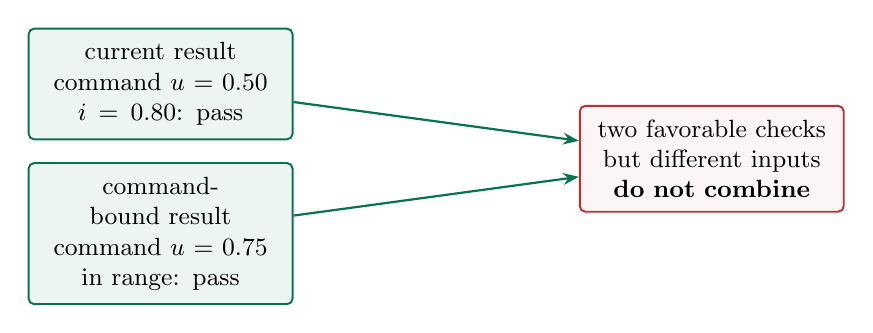
\begin{tikzpicture}
\node[box,text width=3cm] (a) at (0,.95) {current result\\command \(u=0.50\)\\\(i=0.80\): pass};
\node[box,text width=3cm] (b) at (0,-.95) {command-bound result\\command \(u=0.75\)\\in range: pass};
\node[box,text width=3cm,draw=red,fill=red!5] (c) at (7,0) {two favorable checks\\but different inputs\\\textbf{do not combine}};
\draw[arrow] (a)--(c);\draw[arrow] (b)--(c);
\end{tikzpicture}\par
\end{center}
\uncover<2->{Both calculations can be individually correct. Together they do not establish the stated checks for one common candidate.}
\medskip
\uncover<3->{Bind each result to the request revision and command. In L1, changing either makes the old binding fail.}
\Source{Exact request/candidate binding exercise: \href{../Classroom_Labs.ipynb}{L1}.}
\Bridge{What happens when a failed check deliberately sends us backward?}
\note{This deliberately mismatched example shows why a collection of favorable results is not automatically a complete verdict. One result belongs to command 0.50 and the other to command 0.75. Both can be mathematically correct while being inappropriate to combine as evidence for one candidate. The issue is identity, not arithmetic. Ask the class to identify the missing common condition before revealing the binding rule. The classroom implementation later binds request, candidate, and result with hashes and rejects a mismatch. That establishes consistency of recorded data, not source authenticity. The expected interpretation is that a join checks identity as well as completeness. Next, add a repair edge and distinguish the resulting cyclic workflow from the acyclic dependency example.}
\end{frame}

\begin{frame}[t]{A repair loop is a cycle, so give it a stopping rule}
\label{f:F16}
\begin{center}
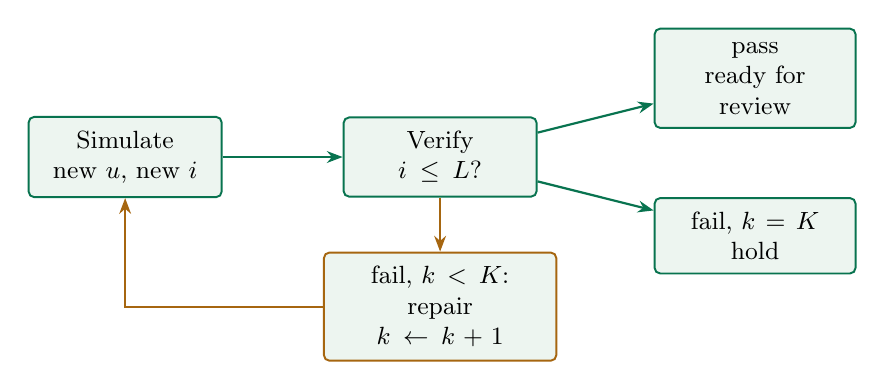
\begin{tikzpicture}
\node[box,text width=2.1cm] (s) at (0,0) {Simulate\\new \(u\), new \(i\)};
\node[box,text width=2.1cm] (v) at (4,0) {Verify\\\(i\leq L\)?};
\node[box,text width=2.2cm] (r) at (8,1) {pass\\ready for review};
\node[box,text width=2.2cm] (h) at (8,-1) {fail, \(k=K\)\\hold};
\node[box,text width=2.6cm,draw=amber] (p) at (4,-1.9) {fail, \(k<K\): repair\\\(k\leftarrow k+1\)};
\draw[arrow] (s)--(v);\draw[arrow] (v)--(r);\draw[arrow] (v)--(h);
\uncover<2->{\draw[arrow,amber] (v)--(p);\draw[arrow,amber] (p.west)-|(s.south);}
\end{tikzpicture}\par
\end{center}
\(k\): completed repairs; \(K\): maximum repairs; both are nonnegative integers. The backward edge makes the program cyclic, not a DAG.
\uncover<3->{The budget bounds attempts if tool calls return. It guarantees neither a feasible command nor a tool timeout.}
\Source{Exact bounded policy: \href{../Graph_Workflow_Lab.ipynb}{G2--G4}; \href{https://docs.langchain.com/oss/python/langgraph/overview}{LangGraph}.}
\Bridge{Can we express those three routes without ambiguity?}
\note{Trace the successful route first and then reveal the backward repair edge. The graph now contains a cycle, so calling it a DAG would be incorrect. A particular completed run can still be drawn as a sequence of visits. The counter k records completed repairs and K is the maximum permitted count. The policy repairs only while k is smaller than K; otherwise a failed verification produces hold. The finite count bounds attempts if each operation returns, but it is separate from a timeout for a stalled solver. Ask whether stopping without a feasible action means the software failed. It may be the correct policy result. The expected interpretation is bounded execution with an explicit unsuccessful outcome. Next, write the routing conditions precisely.}
\end{frame}
\begin{frame}[t]{Route from the verdict and the remaining budget}
\label{f:F17}
\[
r(s)=
\begin{cases}
\texttt{report}, & \text{if passed is true},\\
\texttt{repair}, & \text{if passed is false and } k<K,\\
\texttt{hold}, & \text{otherwise}.
\end{cases}
\]
Here \(s\) is the current record; \(r(s)\) returns one next-node label. \(k\) is the completed repair count and \(K\) is the repair budget.
\medskip
\Question{A failed check has \(k=1\) and \(K=1\). Which route is permitted?}
\Answer{\texttt{hold}. The budget is exhausted; equality does not permit another repair.}
\uncover<3->{Verification computes the verdict. Routing decides what to do with that verdict.}
\Source{The implemented route is four Python lines in \href{../Graph_Workflow_Lab.ipynb}{G2}.}
\Bridge{How should code describe the record that this rule reads?}
\note{Reveal the mutually exclusive conditions in order. The first condition checks whether the latest calculation passed. If it did not, the second decision is whether a repair is still permitted. The route returns a label, and the graph maps that label to a node. This policy is deliberately deterministic so that participants can reason about every execution path. A more flexible language-selected operation could be inserted elsewhere without allowing it to bypass these acceptance conditions. Ask what would happen if the counter were equal to the budget: the route must hold. The numerical verification rule and the orchestration policy remain separate functions.}
\end{frame}

\begin{frame}[t]{A state schema names the facts each node may need}
\label{f:F18}
\begin{tabular}{@{}>{\raggedright\arraybackslash}p{3.1cm}>{\raggedright\arraybackslash}p{3.1cm}>{\raggedright\arraybackslash}p{5.2cm}@{}}
\textbf{Fields} & \textbf{Our example} & \textbf{Purpose}\\\hline
\texttt{command}, \texttt{limit} & \(0.75,\ 0.80\) & identify the trial and unchanged criterion\\
\texttt{current}, \texttt{passed} & \(1.00,\ \texttt{False}\) & store the latest calculation and comparison\\
\texttt{attempts}, \texttt{max\_repairs} & \(0,\ 2\) & decide whether another repair is allowed\\
\texttt{trace} & ordered event list & explain how the current record was reached
\end{tabular}\par
\medskip
\uncover<2->{\(\displaystyle s_{t+1}=\operatorname{merge}(s_t,\Delta s_t)\).
\(s_t\): record before step \(t\); \(\Delta s_t\): returned field updates, not arithmetic subtraction.}
\medskip
\uncover<3->{Python \texttt{TypedDict} describes expected keys and types. The tutorial's \texttt{initial\_state} function performs explicit input-value checks.}
\Source{\href{https://docs.python.org/3/library/typing.html}{Python TypedDict}; validated inputs in \href{../src/graph_workflow_lab.py}{graph-lab helper}.}
\Bridge{Should the next result replace a field or extend it?}
\note{Read the displayed record as a laboratory notebook with named fields. The command identifies what was proposed, the evidence fields identify what was calculated, and the control-flow fields identify what should happen next. The merge expression is a conceptual description of applying returned updates. Delta is not a numerical difference between two entire records. The G notebook uses TypedDict to describe expected keys and types, while its initial-state function explicitly validates numerical inputs. TypedDict itself does not perform runtime value checking. A chat transcript alone is not a substitute for this engineering record because important values and units must be easy to locate and compare.}
\end{frame}

\begin{frame}[t]{A reducer states whether new information replaces or appends}
\label{f:F19}
\begin{columns}[T,onlytextwidth]
\column{.46\textwidth}
\Idea{Replace the current result}{Old current \(1.00\); new current \(0.80\). Store \(0.80\) for the repaired command.}
\uncover<2->{\[
R_{\mathrm{current}}(a,b)=b
\]}
\column{.50\textwidth}
\Idea{Append the event history}{Old list [simulate]; new list [verify]. Store [simulate, verify].}
\uncover<2->{\[
R_{\mathrm{trace}}(a,b)=a+b
\]}
\end{columns}
\(R\) is a reducer; \(a\) is the stored value and \(b\) the returned update. In the right-hand expression, \(+\) means list concatenation.
\medskip
\uncover<3->{Preserve history without pretending an old current is the result for a new command. Parallel writes also need a meaningful merge rule.}
\Source{List reducer in \href{../Graph_Workflow_Lab.ipynb}{G1}; \href{https://docs.langchain.com/oss/python/langgraph/graph-api}{LangGraph reducers}.}
\Bridge{What outcomes should our bounded policy produce before we run it?}
\note{Use the animation to replace the scalar value while visibly extending the event list. The current field describes the latest simulated command, so retaining the old value there would be misleading. The trace field describes history, so discarding earlier events would make the repair difficult to inspect. The example's plus symbol means list concatenation, not arithmetic averaging or consensus. In the code, Annotated attaches the addition function to the trace field. An empty appended list does not erase existing events. If several branches write a field, the application needs a merge rule appropriate to that field and its ordering semantics.}
\end{frame}

\begin{frame}[t]{Three starting states test three distinct paths}
\label{f:F20}
\begin{tabular}{@{}>{\raggedright\arraybackslash}p{2.3cm}>{\raggedright\arraybackslash}p{2.5cm}>{\raggedright\arraybackslash}p{3cm}>{\raggedright\arraybackslash}p{3.6cm}@{}}
\textbf{Start \((u,L,K)\)} & \textbf{First result} & \textbf{After one repair} & \textbf{Expected outcome}\\\hline
\((0.25,0.80,2)\) & \(i=0.60\) & not needed & \uncover<2->{ready immediately}\\
\((0.75,0.80,2)\) & \(i=1.00\) & \(u=0.50,\ i=0.80\) & \uncover<2->{ready after repair}\\
\((0.90,0.50,1)\) & \(i=1.12\) & \(u=0.65,\ i=0.92\) & \uncover<3->{hold: still above limit}
\end{tabular}\par
\medskip
\(u\): command; \(L\): current limit; \(K\): repair budget; \(i=0.4+0.8u\). Repair subtracts \(0.25\), bounded below by zero.
\medskip
The final case is useful: the process stops correctly even though it does not find an acceptable command within its budget.
\Source{These are the exact three cases executed in \href{../Graph_Workflow_Lab.ipynb}{G4}.}
\Bridge{What does LangGraph add to these ordinary Python functions?}
\note{Give the audience time to calculate the three first results before revealing the outcomes. The first starts within its limit and needs no repair. The second is the worked example: one subtraction produces a command of 0.50 and a current of 0.80. The third starts at 1.12, repairs to 0.92, and still exceeds its smaller limit of 0.50. Its one permitted repair has been used, so a hold is correct. We have not run code yet; these are predictions that the later assertions will test. Ask whether a more generous budget changes the third outcome. The expected interpretation is that success, successful repair, and exhausted repair are different paths worth exercising. Next, explain the runtime that connects the functions.}
\end{frame}

\begin{frame}[t]{LangGraph runs the stateful process we have already specified}
\label{f:F21}
\begin{center}
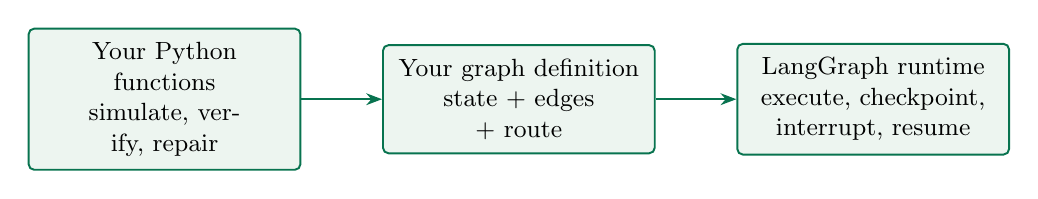
\begin{tikzpicture}
\node[box,text width=3.1cm] (f) at (0,0) {Your Python functions\\simulate, verify, repair};
\node[box,text width=3.1cm] (g) at (4.5,0) {Your graph definition\\state + edges + route};
\node[box,text width=3.1cm] (r) at (9,0) {LangGraph runtime\\execute, checkpoint,\\interrupt, resume};
\draw[arrow] (f)--(g);\draw[arrow] (g)--(r);
\end{tikzpicture}\par
\end{center}
\uncover<2->{The functions still contain the arithmetic. The route still contains the stopping policy. LangGraph makes their execution structure explicit.}
\medskip
\uncover<3->{Our G notebook uses real LangGraph without an LLM or electrical simulator. The engineering notebooks remain custom Python; this is not a claim that they were migrated to LangGraph.}
\Source{\href{https://docs.langchain.com/oss/python/langgraph/overview}{LangGraph overview}; \href{../Graph_Workflow_Lab.ipynb}{executed G notebook}.}
\Bridge{Can everyone confirm the same experiment boundary before running?}
\note{Introduce the package only after the audience understands the process it will execute. LangGraph does not invent the response law or choose the acceptance rule in this example. Those remain ordinary Python functions. The graph definition supplies a state schema, nodes, edges, and a conditional route, while the runtime supports execution and later pause mechanisms. This separation makes it easier to compare the graph with a direct-Python implementation using the same functions. The G notebook is an actual LangGraph exercise, but the larger engineering notebooks use their existing custom orchestration. The expected interpretation is a precise software boundary rather than a package name attached to everything. Next, run setup and inspect the installed versions and the scope statement.}
\end{frame}

\begin{frame}[t]{G0: import the runtime and record what this experiment is}
\label{f:F22}
\Checkpoint{G0}{Run the full setup cell in \texttt{Graph\_Workflow\_Lab.ipynb}.}
\lstinputlisting[style=python,firstline=5,lastline=13]{snippets/G0.py}
\uncover<2->{The printed versions identify the environment. The last line identifies the scope: rule-driven toy execution, with no model call or electrical validation.}
\uncover<3->{After dependencies are installed, this exercise needs neither Ollama nor OpenDSS.}
\Source{Exact notebook lines 5--13: \href{../Graph_Workflow_Lab.ipynb}{G0}; \href{https://docs.langchain.com/oss/python/langgraph/overview}{LangGraph}.}
\Bridge{Which record fields will the runtime carry between nodes?}
\note{Run the complete G0 cell, even though the slide displays only its relevant lines. Confirm that the version dictionary appears before proceeding. The captured run used LangGraph 1.2.15, checkpoint 4.3.0, and langchain-core 1.6.12; a participant's environment may differ. The cell disables the external tracing flags used by this exercise and declares that no language-model or electrical-model validation occurs. After dependencies are installed, the toy needs no Ollama service. If imports fail, use the supplied graph-lab requirements and return to the documented setup rather than changing the experiment during class. This practical boundary keeps the graph lesson reproducible. The expected interpretation is to identify the input, returned evidence, and next permitted step before discussing the final status.}
\end{frame}

\begin{frame}[t]{G1: the schema is our before-and-after table in Python}
\label{f:F23}
\Checkpoint{G1}{Run the full cell; connect each field to the worked example.}
\begin{columns}[T,onlytextwidth]
\column{.47\textwidth}
\lstinputlisting[style=python,firstline=1,lastline=10]{snippets/G1.py}
\column{.49\textwidth}
\Idea{Trial and gate}{\texttt{command}, \texttt{limit}, \texttt{current}, and \texttt{passed} record the comparison.}
\uncover<2->{\Idea{Execution history}{\texttt{attempts} counts repairs. \texttt{trace} appends event lists using \texttt{add}.}}
\uncover<3->{\texttt{TypedDict} describes the schema; input validation is performed separately.}
\end{columns}
\Source{Exact state schema: \href{../Graph_Workflow_Lab.ipynb}{G1}; \href{https://docs.python.org/3/library/typing.html}{TypedDict}.}
\Bridge{Where does the formula become an executable node?}
\note{Highlight the control fields first, then the verdict fields, then the trace annotation. Run the complete G1 cell so the audience also sees the initial validated state and the list-addition example below this excerpt. TypedDict states the intended record structure; initial\_state performs the example's explicit input validation. These two mechanisms should not be confused. The trace is a sequence of recorded events, not an internal chain of thought and not a cryptographically authenticated audit log. Ask participants to predict the number of trace entries before revealing the answer. This is the same replace-versus-append idea they saw conceptually. The expected interpretation is to identify the input, returned evidence, and next permitted step before discussing the final status.}
\end{frame}

\begin{frame}[t]{G2: simulation returns a number; verification returns a verdict}
\label{f:F24}
\Checkpoint{G2}{Run the whole cell; these are its first two node functions.}
\lstinputlisting[style=python,firstline=1,lastline=7]{snippets/G2.py}
\begin{columns}[T,onlytextwidth]
\column{.47\textwidth}
\uncover<2->{\Idea{Simulation update}{For \(u=0.75\), return \texttt{current = 1.00} and an event.}}
\column{.49\textwidth}
\uncover<3->{\Idea{Verification update}{Compare \(1.00\) with \(0.80\); return \texttt{passed = False} and another event.}}
\end{columns}
The \(10^{-12}\) code tolerance addresses floating-point comparison in this toy; it is not an engineering operating margin.
\Source{Exact functions: \href{../Graph_Workflow_Lab.ipynb}{G2, lines 1--7}.}
\Bridge{How does a failed comparison become a repair rather than an uncontrolled loop?}
\note{Read the first function as an ordinary Python calculation. It returns current and a trace update rather than reconstructing the entire state record. The next function compares that current with the limit using a small numerical tolerance. The tolerance addresses floating-point comparison in this toy; it is not an engineering margin. With command 0.75, the result is 1.00 and the limit is 0.80, so the verdict is false. That outcome is expected rather than a program error. Ask which returned field the router will inspect. Run the entire G2 cell, including the repair and terminal-node definitions that follow this excerpt.}
\end{frame}

\begin{frame}[t]{G2: repair changes the command; routing checks the budget}
\label{f:F25}
\begin{columns}[T,onlytextwidth]
\column{.50\textwidth}
\textbf{Change the command and count the repair}
\lstinputlisting[style=python,firstline=9,lastline=11]{snippets/G2.py}
\column{.46\textwidth}
\textbf{Choose the permitted next node}
\lstinputlisting[style=python,firstline=19,lastline=22]{snippets/G2.py}
\end{columns}
\uncover<2->{The command drops by \(0.25\), bounded below by zero; \texttt{attempts} increases by one. Neither line changes the limit.}
\medskip
\uncover<3->{A pass returns \texttt{report}. Otherwise, the route returns \texttt{repair} only while the counter is smaller than its maximum.}
\Source{Exact repair and route: \href{../Graph_Workflow_Lab.ipynb}{G2, lines 9--11 and 19--22}.}
\Bridge{Which graph edge forces a repaired command to be simulated again?}
\note{Read the two functions as separate responsibilities. Repair computes a changed command and records that an attempt has been used. Route reads the most recent verdict and decides which node may execute next. Neither function relaxes the current limit. With the worked starting command, one repair changes 0.75 to 0.50 and increments the counter from zero to one. The new command still requires simulation and verification before it can report ready. Ask what route is returned after a failed check with one attempt used and a maximum of one. The answer is hold. The expected interpretation is that the stopping policy is visible in four lines, rather than hidden in a prompt. Next, connect these functions using the graph's actual edges.}
\end{frame}

\begin{frame}[t]{G3: the backward edge makes every repair face a fresh calculation}
\label{f:F26}
\Checkpoint{G3}{Run the cell and inspect the compiled node list.}
\lstinputlisting[style=python,firstline=7,lastline=14]{snippets/G3.py}
\uncover<2->{\texttt{simulate} \(\rightarrow\) \texttt{verify} always calculates before checking. The conditional edge reads the label returned by \texttt{route}.}
\uncover<3->{\texttt{repair} \(\rightarrow\) \texttt{simulate} is the return loop. Compilation checks structure; it does not prove the response law or its physical assumptions.}
\Source{Exact graph wiring: \href{../Graph_Workflow_Lab.ipynb}{G3}; \href{https://docs.langchain.com/oss/python/langgraph/use-graph-api}{LangGraph construction}.}
\Bridge{Do the three executions match our hand calculations?}
\note{Run G3 and confirm the compiled node list. Highlight the fixed edge from simulate to verify, the conditional edge that calls route, and the edge returning repair to simulate. The mapping translates a returned label into a permitted successor. The report and hold nodes terminate this version of the execution. Compilation checks structural requirements of the graph; it is not a proof that the chosen response law describes a feeder or that the repair rule finds an optimum. This keeps the software lesson separate from the later numerical science. Ask a participant to point to the line that makes the graph cyclic.}
\end{frame}

\begin{frame}[t]{G4: predict, run, then explain one complete trace}
\label{f:F27}
\Checkpoint{G4}{Run unchanged, then use a separate scratch cell for a new budget.}
\begin{tabular}{@{}llll@{}}
\textbf{Case} & \textbf{Final command} & \textbf{Final current} & \textbf{Status}\\\hline
Already admissible & \(0.25\) & \(0.60\) & \texttt{TOY\_READY}\\
One repair & \(0.50\) & \(0.80\) & \texttt{TOY\_READY}\\
Budget exhausted & \(0.65\) & \(0.92\) & \texttt{TOY\_HOLD}
\end{tabular}\par
\medskip
\uncover<2->{\textbf{Repair trace:}
simulate \(1.00\) \(\rightarrow\) verify false \(\rightarrow\) repair
\(\rightarrow\) simulate \(0.80\) \(\rightarrow\) verify true \(\rightarrow\) report.}
\medskip
\Question{What if the exhausted case gets four repairs instead of one?}
\Answer{It reaches \(u=0\), hence \(i=0.40\leq0.50\), and can report ready.}
\Source{Exact outputs, trace assertion, and cases: \href{../Graph_Workflow_Lab.ipynb}{G4}.}
\Bridge{Did graph execution improve the command over conventional Python?}
\note{Give participants time to predict before running. The first case passes immediately. The second begins at current 1.00, reduces the command from 0.75 to 0.50, and then reaches current 0.80. The third begins at command 0.90, repairs to 0.65, and still exceeds its 0.50 limit with current 0.92. Its single repair is exhausted, so hold is correct. Run G4 unchanged because its assertions describe these original three cases. For a new limit or repair budget, invoke the graph in a separate scratch cell. A useful extension gives the third case four repairs: it reaches command zero and current 0.40. The expected interpretation is to identify the input, returned evidence, and next permitted step before discussing the final status.}
\end{frame}

\begin{frame}[t]{G4: hold the functions fixed and compare the supervisor}
\label{f:F28}
\lstinputlisting[style=python,firstline=15,lastline=19]{snippets/G4.py}
\begin{columns}[T,onlytextwidth]
\column{.47\textwidth}
\Idea{Controlled comparison}{Same initial states, response law, repair rule, verification, and route.}
\column{.49\textwidth}
\uncover<2->{\Idea{Observed result}{All three commands, statuses, and event histories match the direct-Python baseline.}}
\end{columns}
\uncover<3->{The graph did not improve this toy control result. Its explicit structure supports inspection and the pause/resume mechanism we will test next.}
\Source{Executable baseline equality assertion: \href{../Graph_Workflow_Lab.ipynb}{G4, lines 15--19}.}
\Bridge{How can a ready calculation wait for a person's response?}
\note{Make the null numerical result a central teaching outcome. Both implementations receive the same initial state and the same node functions. The comparison asserts equality of the summary, including the command, status, and trace. Therefore the graph should not be credited with finding a better action. Its value here is making execution structure and later checkpoint mechanisms explicit. The notebook prints elapsed times from one local execution, but those values are not a statistically controlled performance benchmark. Differences at this scale depend on runtime and measurement overhead. Ask which separate experiment would support an inspectability or recovery claim. The expected interpretation is to identify the input, returned evidence, and next permitted step before discussing the final status.}
\end{frame}
\begin{frame}[t]{A checkpoint preserves the record and the next unfinished step}
\label{f:F29}
\begin{center}
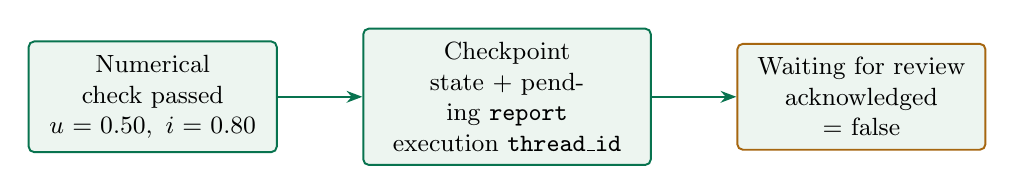
\begin{tikzpicture}
\node[box,text width=2.8cm] (a) at (0,0) {Numerical check passed\\\(u=0.50,\ i=0.80\)};
\node[box,text width=3.3cm] (b) at (4.5,0) {Checkpoint\\state + pending \texttt{report}\\execution \texttt{thread\_id}};
\node[box,text width=2.8cm,draw=amber] (c) at (9,0) {Waiting for review\\acknowledged = false};
\draw[arrow] (a)--(b);\draw[arrow] (b)--(c);
\end{tikzpicture}\par
\end{center}
\uncover<2->{A checkpoint is a saved execution record. A thread identifier associates a later response with that execution; it is not an operator credential.}
\medskip
\uncover<3->{The lab uses \texttt{InMemorySaver}. It supports a pause within the running kernel, not durable recovery after the process is lost.}
\Source{\href{https://docs.langchain.com/oss/python/langgraph/persistence}{LangGraph persistence}; actual checkpoint inspection: \href{../Graph_Workflow_Lab.ipynb}{G5}.}
\Bridge{What exactly is sent to the reviewer, and what response is accepted?}
\note{Use a bookmark analogy, then make it precise with the stored record and pending node. In the G lab, a thread identifier associates the checkpoint with a particular execution. That identifier is not an operator credential. The example uses InMemorySaver, so the state remains available in the running process but does not provide durable recovery after the kernel disappears. This scope is sufficient for observing a pause and resume during class. Participants should inspect the snapshot before discussing its final status; otherwise a whole-cell execution can make the pause easy to miss. The upcoming exercise prints the pending node and acknowledgment flag.}
\end{frame}

\begin{frame}[t]{G5: interrupt with the recommendation that needs a response}
\label{f:F30}
\lstinputlisting[style=python,firstline=1,lastline=9]{snippets/G5.py}
\uncover<2->{The payload states the command, toy consequence, recommendation identity, and scope. A matching approval is required to record acknowledgment.}
\uncover<3->{On resume, the node can run again from its beginning. Do not put an uncontrolled equipment action before the interrupt.}
\Source{Exact review function: \href{../Graph_Workflow_Lab.ipynb}{G5, lines 1--9}; \href{https://docs.langchain.com/oss/python/langgraph/interrupts}{interrupt semantics}.}
\Bridge{Can we see the paused state before the response is supplied?}
\note{Distinguish a visible recommendation from an acknowledged recommendation. The toy sends an interrupt payload that includes a recommendation identifier, command, calculated value, and declared scope. Its scripted reply must approve the same identifier. A wrong identifier or a declined response remains distinguishable from approval. This demonstrates a record-consistency mechanism, not operator authentication or equipment dispatch. On resumption, the interrupted node can begin again, so uncontrolled side effects before the interrupt would be a design problem. The toy only records state changes. Ask participants what the operator should see if the candidate changes while review is pending. The answer motivates fresh evidence and a new identity.}
\end{frame}

\begin{frame}[t]{G5: pause and inspect before resuming}
\label{f:F31}
\Checkpoint{G5}{For a visible pause, execute lines 1--17 first; then inspect the output.}
\lstinputlisting[style=python,firstline=11,lastline=17]{snippets/G5.py}
\uncover<2->{\textbf{Expected pre-resume output:} pending node \texttt{('report',)}; \texttt{acknowledged: False}. The payload describes the exact toy recommendation.}
\uncover<3->{Running the full cell also supplies a scripted response afterward. Inspect both printed stages rather than overlooking the intermediate pause.}
\Source{Exact pause and snapshot: \href{../Graph_Workflow_Lab.ipynb}{G5, lines 11--17}.}
\Bridge{How does the matching response change the saved execution?}
\note{The full G5 cell both pauses and supplies a scripted response, so explain how to observe the intermediate state. For a live teaching pause, execute lines 1 through 17 first, retaining the function definition above this displayed excerpt. Inspect the printed pending node, which is report, and the false acknowledgment flag. The interrupt payload identifies the command and the invented model scope. In the captured pause, the stored status remains TOY\_NEW; it should not be mislabeled TOY\_READY merely because the numerical gate passed. The checkpoint exists in this kernel's memory. Participants can now see that a verified numerical result and an acknowledged recommendation are different states.}
\end{frame}

\begin{frame}[t]{G5: resume the same execution with a matching readback}
\label{f:F32}
\lstinputlisting[style=python,firstline=18,lastline=21]{snippets/G5.py}
\begin{columns}[T,onlytextwidth]
\column{.47\textwidth}
\uncover<2->{\Idea{Matching simulated approval}{Status becomes \texttt{TOY\_ACKNOWLEDGED}; no node remains pending.}}
\column{.49\textwidth}
\uncover<3->{\Idea{Decline or wrong identity}{The review function returns \texttt{TOY\_HOLD}; acknowledgment remains false.}}
\end{columns}
This is a state-management exercise. The scripted response does not authenticate a person, and the example sends no equipment command.
\Source{Exact resume and final assertion: \href{../Graph_Workflow_Lab.ipynb}{G5}; \href{https://docs.langchain.com/oss/python/langgraph/interrupts}{LangGraph interrupts}.}
\Bridge{What if the request changes while an old result remains available?}
\note{Execute the remaining lines after the pause, or inspect both printed stages if participants ran the full cell. The response is explicitly simulated and generated by the notebook, not provided by an authenticated operator. Its identifier must match the recommendation constructed from the saved state. The resumed graph records acknowledgment and has no pending node. To discuss rejection, point to the human\_review function: it requires an approval value of true and the correct identifier; otherwise it returns hold. Avoid resuming an already completed execution for this experiment; create a fresh review run before trying a different response. No equipment endpoint is present.}
\end{frame}

\begin{frame}[t]{L1: a changed request must not reuse old evidence}
\label{f:F33}
\Checkpoint{L0--L1}{Open \texttt{Classroom\_Labs.ipynb}; run setup and the binding experiment.}
\lstinputlisting[style=python,firstline=1,lastline=5]{snippets/L1.py}
\begin{tabular}{@{}>{\raggedright\arraybackslash}p{8cm}l@{}}
Same request and same command & \uncover<2->{\texttt{True}}\\
Changed load; old evidence & \uncover<2->{\texttt{False}}\\
Changed command; old evidence & \uncover<2->{\texttt{False}}
\end{tabular}\par
\medskip
\uncover<3->{The payload is explicitly \texttt{example\_only}. Hash binding checks consistency; it does not prove physical feasibility or source authenticity.}
\Source{Exact inputs and expected outputs: \href{../Classroom_Labs.ipynb}{L1}; \href{../src/classroom_labs.py}{binding implementation}.}
\Bridge{Which other checks must remain separate from evidence identity?}
\note{Allow four minutes for setup, prediction, execution, and explanation. The initial request uses load scale 1.00, rating fraction 0.80, and revision one. L1 changes the load to 1.10 and revision to two, then separately tests a changed command. The expected binding results are true, false, and false. The payload is deliberately marked example\_only; this is an evidence-identity experiment, not a fresh feeder solve. A matching hash establishes consistency among these recorded inputs and the bound result. It does not establish source authenticity, correct intent, or physical feasibility. Fixed supervisors can use the same guard, so the test demonstrates an implementable workflow property without claiming an exclusive LLM benefit.}
\end{frame}

\begin{frame}[t]{Schema, binding, and engineering checks answer different questions}
\label{f:F34}
\begin{tabular}{@{}>{\raggedright\arraybackslash}p{2cm}>{\raggedright\arraybackslash}p{4.1cm}>{\raggedright\arraybackslash}p{5.5cm}@{}}
\textbf{Check} & \textbf{Question} & \textbf{A pass does not establish}\\\hline
Schema & Are required fields and values valid? & Correct interpretation of the operator's intent\\
Binding & Does this result belong to this candidate? & Authenticity of its source\\
Engineering & Do modeled limits pass? & Adequate model scope or field authorization
\end{tabular}\par
\medskip
\Question{A solver converges at \(112\) A; the declared limit is \(100\) A. Two LLMs favor the candidate. Accept it?}
\Answer{No. The current check fails by \(12\) A. A vote cannot raise the declared limit.}
\Source{Tutorial evidence and limit checks: \href{../src/classroom_labs.py}{classroom tools}; \href{../src/proposal_case_tools.py}{case adapters}.}
\Bridge{Two similar acronyms now appear: what is MCP, and what is MPC?}
\note{Keep this slide concrete rather than reading a compliance checklist. Give the current example verbally and ask for the verdict before revealing it. A converged solver result can fail a physical operating condition. A correctly shaped result can be stale. A matching hash can identify consistent data without proving who produced it. These checks are complementary because they answer different questions. Our later lab uses an explicitly illustrative payload to isolate the binding mechanism; participants must not mistake its passed field for a real feeder calculation. The final operator packet adds another distinction between evidence scope and the requested scope.}
\end{frame}

\begin{frame}[t]{MCP connects tools; MPC computes a control plan}
\label{f:F35}
\begin{columns}[T,onlytextwidth]
\column{.47\textwidth}
\textbf{MCP: Model Context Protocol}
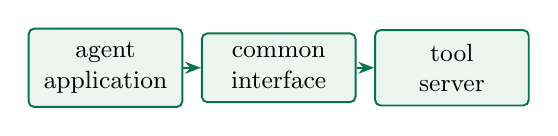
\begin{tikzpicture}
\node[box,text width=1.6cm] (a) at (0,0) {agent\\application};
\node[box,text width=1.6cm] (b) at (2.2,0) {common\\interface};
\node[box,text width=1.6cm] (c) at (4.4,0) {tool\\server};
\draw[arrow] (a)--(b);\draw[arrow] (b)--(c);
\end{tikzpicture}\par
It standardizes tool discovery, arguments, and results. It does not determine whether a current is acceptable.
\column{.49\textwidth}
\uncover<2->{\textbf{MPC: Model Predictive Control}
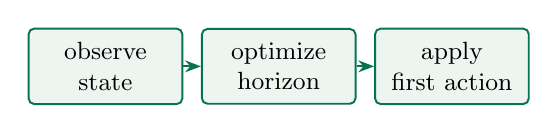
\begin{tikzpicture}
\node[box,text width=1.6cm] (a) at (0,0) {observe\\state};
\node[box,text width=1.6cm] (b) at (2.2,0) {optimize\\horizon};
\node[box,text width=1.6cm] (c) at (4.4,0) {apply\\first action};
\draw[arrow] (a)--(b);\draw[arrow] (b)--(c);
\end{tikzpicture}\par
It uses a predictive model, objective, and constraints to plan control, then replans after the next observation.}
\end{columns}
\medskip
\uncover<3->{An MPC solver could be exposed through MCP. Our classroom functions are called directly in Python; the tutorial does not require an MCP server.}
\Source{\href{https://modelcontextprotocol.io/specification/2025-11-25/server/tools}{MCP tools specification}; \href{https://sites.engineering.ucsb.edu/~jbraw/mpc/}{Rawlings et al., MPC}.}
\Bridge{How do MPC and a learned policy produce candidates differently?}
\note{Spell out both acronyms and contrast their purposes using the two drawings. MCP is a communication interface for tools. MPC is a numerical control method that predicts behavior and optimizes a sequence of actions. The similarity of their letters does not imply a mathematical connection. A solver implementing MPC can be exposed as a tool through an MCP server, but the interface does not replace the objective, constraints, or verification. Our classroom notebook calls Python functions directly and does not claim to demonstrate an MCP server. Ask which component would compute a control sequence and which would describe how to call that component. The expected interpretation is a clean separation between interoperability and control. Next, compare optimization-based planning with a learned continuous-action policy.}
\end{frame}

\begin{frame}[t]{MPC plans with a model; SAC supplies a learned continuous action}
\label{f:F36}
\begin{columns}[T,onlytextwidth]
\column{.48\textwidth}
\textbf{Model-based planning}
\[
\min_{u_{0:H-1}}\sum_{k=0}^{H-1}\ell(x_k,u_k)
\]
subject to a prediction model and operating constraints. Apply the first action, observe again, and replan.
\column{.48\textwidth}
\uncover<2->{\textbf{Model-free policy inference}
\[
u_t=\pi_\theta(o_t).
\]
The trained policy maps an observation to a continuous command. Class uses saved SAC weights; it does not train a new actor.}
\end{columns}
\small
\(H\): planning horizon; \(k\): predicted step; \(x_k\): predicted state; \(u_k\): control; \(\ell\): stage cost. \(t\): current decision time; \(o_t\): observation; \(\pi_\theta\): policy with learned parameters \(\theta\).
\medskip
\uncover<3->{\textbf{Same acceptance process:} simulate both candidates and check the same declared limits. PPO is discussed as an alternative; it is not trained here.}
\Source{\href{https://sites.engineering.ucsb.edu/~jbraw/mpc/}{MPC}; \href{https://proceedings.mlr.press/v80/haarnoja18b.html}{SAC}; \href{https://arxiv.org/abs/1707.06347}{PPO}.}
\Bridge{Which research frameworks already organize related grid work?}
\note{Define the two broad approaches before naming the particular algorithms. Model-based control uses predicted behavior in an optimization problem; the displayed expression omits constraints for clarity, and the voltage lesson supplies them explicitly. Model-free learning trains an action rule through experience and rewards. It may obtain that experience from a simulator, so model-free does not mean no simulator was used. MPC plans over a horizon and applies its first action. SAC supplies continuous control from saved learned weights in class. PPO is a relevant continuous-action alternative but is not trained in this tutorial. Training cost and inference cost are separate. Both proposed commands must be simulated and checked under the same declared limits.}
\end{frame}

\begin{frame}[t]{Prior frameworks contribute mechanisms we can teach and test}
\label{f:F37}
\small
\begin{tabular}{@{}>{\raggedright\arraybackslash}p{2.6cm}>{\raggedright\arraybackslash}p{4.1cm}>{\raggedright\arraybackslash}p{4.9cm}@{}}
\textbf{Framework} & \textbf{Useful mechanism} & \textbf{Connection to our example}\\\hline
PowerAgent ecosystem & reusable engineering interfaces and workflows & expose the calculation with inspectable inputs and outputs\\
PowerDAG & exemplar retrieval; prerequisite advisory & detect a covered dependency problem before a tool call\\
Grid-Agent v3 & specialized roles; sandbox validation and rollback & keep a failed trial separate from the incumbent\\
X-GridAgent & planning--coordination--action hierarchy & preserve task context across handoffs
\end{tabular}\par
\medskip
\uncover<2->{PowerDAG covers selected rules and permits repeated calls after its one-shot advisory. That mechanism is not an unconditional hard safety gate.}
\uncover<3->{These are close prior works, not a leaderboard. Our tutorial does not claim the first multi-agent grid workflow or first use of numerical verification.}
\Source{\href{https://poweragent.seas.harvard.edu/}{PowerAgent}; \href{https://arxiv.org/html/2603.17418v1}{PowerDAG}; \href{https://arxiv.org/html/2508.05702v3}{Grid-Agent v3}; \href{https://arxiv.org/html/2512.20789v1}{X-GridAgent}.}
\Bridge{How can a compact comparison keep these qualifications visible?}
\note{After the concrete examples, the audience can now connect literature mechanisms to work they understand. PowerAgent organizes domain capabilities through interfaces and workflows. PowerDAG uses retrieved exemplars and a prerequisite supervisor whose inspected version covers selected rules and allows a repeated call after a one-shot advisory. Grid-Agent separates roles and evaluates changes with validation and rollback. X-GridAgent separates planning, coordination, and action. The point is to identify design ideas rather than compare incompatible success percentages. These works are close prior art, so the tutorial should not claim to invent role decomposition or numerical checking. The expected interpretation is a mechanism-focused literature map. Next, use a small tick matrix while preserving the qualifications a tick alone could hide.}
\end{frame}

\begin{frame}[t]{A capability tick describes documented scope, not superiority}
\label{f:F38}
\fontsize{8.5}{10}\selectfont
\begin{tabular}{@{}>{\raggedright\arraybackslash}p{3cm}cccc>{\raggedright\arraybackslash}p{3.9cm}@{}}
\textbf{Work} & \textbf{Tools} & \textbf{Feedback} & \textbf{Checks} & \textbf{Review} & \textbf{Qualification}\\\hline
PowerAgent & \(\checkmark\) & \(\checkmark\) & \(\triangle\) & \(\checkmark\) & capabilities depend on workflow\\
PowerDAG & \(\checkmark\) & \(\checkmark\) & \(\triangle\) & NR & selected rules; one-shot advisory\\
Grid-Agent v3 & \(\checkmark\) & \(\checkmark\) & \(\checkmark\) & \(\triangle\) & sandbox; deployment oversight proposed\\
X-GridAgent & \(\checkmark\) & \(\checkmark\) & \(\triangle\) & \(\triangle\) & solver checks; prompt refinement\\
PowerAgentBench-SS & \(\checkmark\) & \(\checkmark\) & \(\checkmark\) & \(\triangle\) & DC benchmark; hidden revalidation\\
Tutorial & \(\checkmark\) & \(\checkmark\) & \(\checkmark\) & \(\checkmark\) & declared models; local readback
\end{tabular}\par
\smallskip
\(\checkmark\): documented; \(\triangle\): qualified or proposed; NR: not reported in the inspected source. Benchmark work evaluates agents; it is not itself a controller.
\uncover<2->{Common scenarios, tools, budgets, and outcome definitions are needed before claiming an advantage.}
\Source{\href{https://poweragent.seas.harvard.edu/}{PowerAgent}; \href{https://arxiv.org/html/2603.17418v1}{PowerDAG}; \href{https://arxiv.org/html/2508.05702v3}{Grid-Agent v3}; \href{https://arxiv.org/html/2512.20789v1}{X-GridAgent}; \href{https://arxiv.org/html/2606.18789v1}{PowerAgentBench-SS}.}
\Bridge{What measurements will separate control benefit from workflow benefit?}
\note{Define the marks before interpreting the rows. A tick records a documented capability in the inspected source; a triangle preserves a qualification; NR means not reported in that source rather than proved absent. PowerAgent capabilities vary by workflow. PowerDAG covers selected dependencies with a one-shot advisory. Grid-Agent oversight is proposed for deployment. X-GridAgent includes solver checks and human prompt refinement. PowerAgentBench-SS supplies an evaluation protocol with hidden revalidation under a DC scope. The tutorial's review tick refers to local advisory readback, not authenticated field authorization. None of these rows forms a shared performance benchmark. Ask what would make a valid benefit claim: common scenarios, tools, budgets, outcome definitions, and timing boundaries.}
\end{frame}

\begin{frame}[t]{Compare benefit in three columns, with the same experiment}
\label{f:F39}
\begin{columns}[T,onlytextwidth]
\column{.31\textwidth}
\Idea{Numerical outcome}{Objective value, served load, constraint violations, and model scope.}
\column{.31\textwidth}
\uncover<2->{\Idea{Workflow outcome}{Stale evidence rejected, required checks recorded, and recommendation identity preserved.}}
\column{.31\textwidth}
\uncover<3->{\Idea{Cost of the decision}{Solver time, model-call time, number of trials, and training cost reported separately.}}
\end{columns}
\medskip
The G baseline already gives a useful null result: the commands tie exactly. That result demonstrates graph mechanics, not better physical control.
\medskip
For the engineering comparison, hold the scenario, available controls, objective, constraints, and trial budget fixed where a paired claim is made.
\Source{Tutorial matched baseline: \href{../Graph_Workflow_Lab.ipynb}{G4}; evaluation design: \href{https://arxiv.org/html/2606.18789v1}{PowerAgentBench-SS}.}
\Bridge{Which parts of this toy transfer to an actual voltage-support study?}
\note{Ask the audience to place a claim in one of the three columns before accepting it. A smaller objective is a numerical claim. Rejection of a stale result is a workflow claim. Faster completion is a timing claim. One does not establish the others. The toy's matching commands demonstrate that graph execution can preserve a conventional policy, but do not demonstrate better control. Later comparisons must disclose common scenarios, candidate budgets, model scope, and the boundary of measured time. Training a controller and running inference are different costs, as are a saved language-model reply and a new call. The expected interpretation is a disciplined way to assess useful, null, or worse outcomes. Next, replace the invented response law with the two declared electrical models.}
\end{frame}

\begin{frame}[t]{Keep the process; replace the toy law with electrical models}
\label{f:F40}
\begin{center}
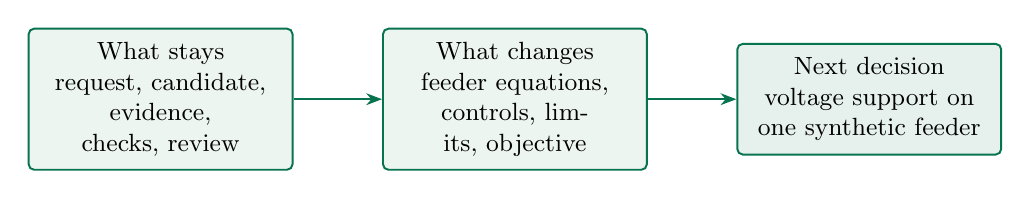
\begin{tikzpicture}
\node[box,text width=3cm] (a) at (0,0) {What stays\\request, candidate,\\evidence, checks, review};
\node[box,text width=3cm] (b) at (4.5,0) {What changes\\feeder equations,\\controls, limits, objective};
\node[box,text width=3cm,fill=teal!10] (c) at (9,0) {Next decision\\voltage support on\\one synthetic feeder};
\draw[arrow] (a)--(b);\draw[arrow] (b)--(c);
\end{tikzpicture}\par
\end{center}
\uncover<2->{MPC and SAC will propose inverter commands. Three-phase LinDistFlow and OpenDSS will expose differences in modeled consequences and scope.}
\medskip
\uncover<3->{Llama's bounded choices, public explanations, and latency will be inspected alongside numerical baselines. A favorable explanation never substitutes for a fresh check.}
\Source{Voltage experiments and exact outputs: \href{../Classroom_Labs.ipynb}{L2--L5}; response traces: \href{../results/proposal_complete_workflow.json}{five-stage archive}.}
\Bridge{What do active and reactive inverter commands do to feeder voltage?}
\note{Recap the transferable mechanisms in one sentence: state records the case, tools return evidence, routes handle success and repair, and review records a response to a particular recommendation. The G lab established those mechanisms but did not establish grid-control performance. The engineering notebook now switches to actual numerical models and recorded model responses. Keep the comparison fair by fixing the scenario, permitted controls, declared constraints, objective, and candidate budget wherever a paired comparison is claimed. Report changes in model scope explicitly rather than treating them as unexplained error. The next section introduces the electrical meaning of active and reactive control before displaying the optimization.}
\end{frame}

\section{Voltage support: continuous control}
% Compact chapter-local teaching panels; global theme is unchanged.
\newcommand{\VoltageIdea}[2]{\par\smallskip\begin{beamercolorbox}[sep=.8mm,wd=\linewidth]{block body}{\color{teal}\bfseries #1\par}#2\end{beamercolorbox}\par}

\begin{frame}[t]{The operator's question: how much PV can this feeder accept?}
\label{f:V01}
\small

\begin{columns}[T]
\column{.47\textwidth}
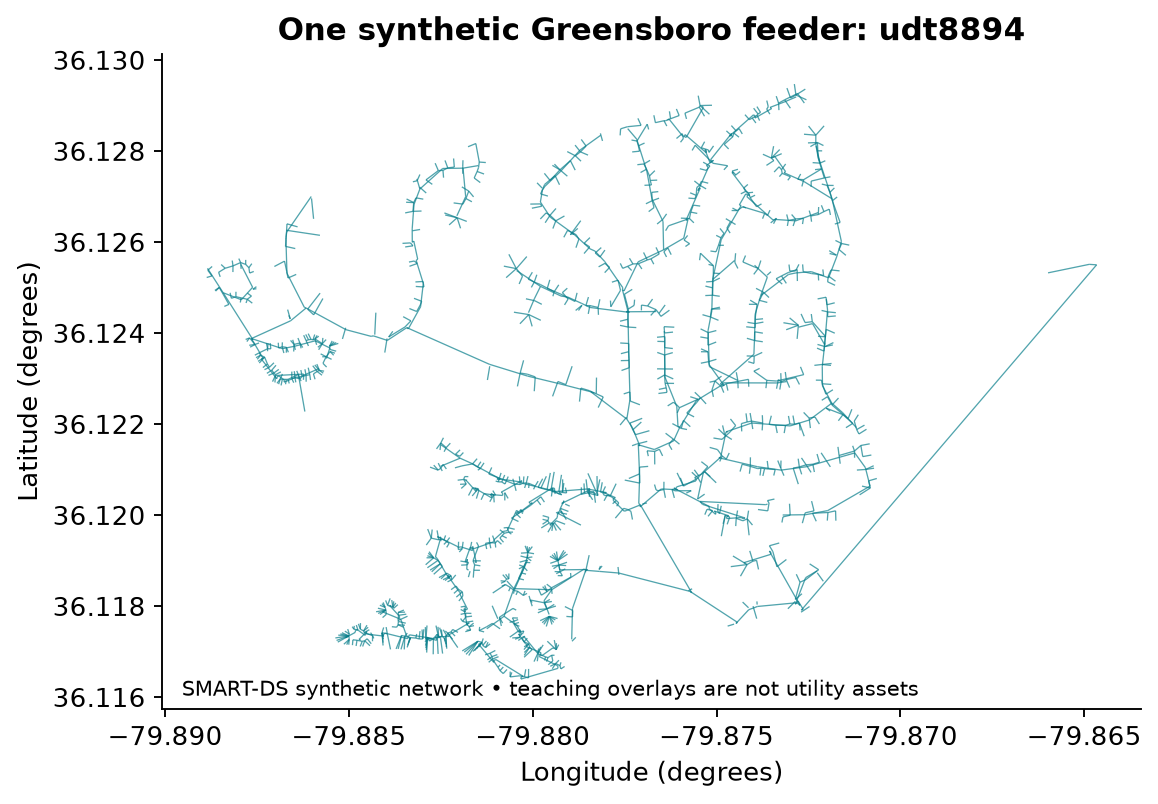
\includegraphics[width=\linewidth,height=3.75cm,keepaspectratio]{figures/feeder.png}
{\scriptsize One SMART-DS synthetic Greensboro feeder:\\ \texttt{uhs20\_1247--udt8894}.}
\column{.50\textwidth}
\VoltageIdea{An operating request}{Use available PV while keeping modeled voltages and currents within their limits.}
\medskip
\par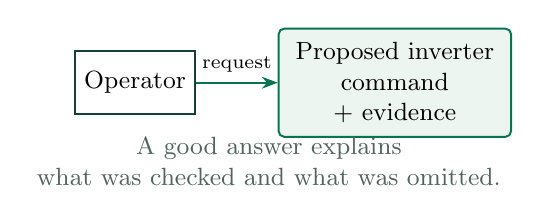
\begin{tikzpicture}[x=1cm,y=1cm]
\node[draw=navy,thick,minimum width=1.1cm,minimum height=.8cm] (op) at (0,0) {\small Operator};
\node[box,text width=2.6cm] (rec) at (3.3,0) {Proposed inverter\\command + evidence};
\draw[arrow] (op)--node[above,font=\scriptsize]{request}(rec);
\node[font=\small,text=slate,align=center] at (1.7,-1) {A good answer explains\\what was checked and what was omitted.};
\end{tikzpicture}\par
\uncover<2->{\Question{Which could limit additional PV: voltage, current, or inverter capability?}
\Answer{Any of the three. We must inspect their margins together.}}
\end{columns}

\Source{\href{https://data.openei.org/submissions/2981}{SMART-DS synthetic distribution models}; Executed \texttt{Classroom\_Labs.ipynb}; \texttt{src/classroom\_labs.py}}
\Bridge{What physical path connects the PV inverter to the source?}
\note{The voltage chapter uses one SMART-DS synthetic Greensboro feeder, identified as uhs20\_1247--udt8894. It is not a model of the whole city or a live utility. Ask learners which information they still need before advising an operator: device availability, thermal ratings, voltage bounds, model coverage and permitted actions. The map establishes geographic context; it does not establish operational validity. Our numerical experiment uses a fleet command with two continuous variables. All recommendations remain advisory simulation outputs. This chapter moves from a familiar control problem to the reason for explicit agent handoffs: a recommendation should carry the evidence and assumptions that justify it.}
\end{frame}

\begin{frame}[t]{See the electrical path before choosing an algorithm}
\label{f:V02}
\small

\begin{center}
\par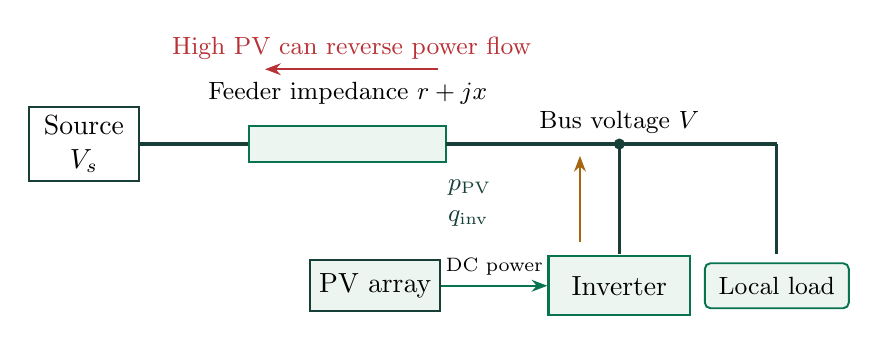
\begin{tikzpicture}[x=1cm,y=1cm]
\node[draw=navy,thick,minimum width=1.4cm,minimum height=.9cm,align=center] (src) at (0,0) {Source\\$V_s$};
\coordinate (b) at (6.8,0);
\draw[very thick,navy] (src.east)--(2.1,0);
\draw[thick,teal,fill=pale] (2.1,-.23) rectangle (4.6,.23);
\node[font=\small] at (3.35,.65) {Feeder impedance $r+jx$};
\draw[very thick,navy] (4.6,0)--(8.8,0);
\fill[navy] (b) circle (2pt);
\node[above,font=\small] at (b) {Bus voltage $V$};
\draw[very thick,navy] (8.8,0)--(8.8,-1.4);
\node[box] at (8.8,-1.8) {Local load};
\draw[very thick,navy] (b)--(6.8,-1.4);
\node[draw=teal,thick,fill=pale,minimum width=1.8cm,minimum height=.75cm] (inv) at (6.8,-1.8) {Inverter};
\node[draw=navy,fill=pale,minimum width=1.5cm,minimum height=.65cm] (pv) at (3.7,-1.8) {PV array};
\draw[arrow] (pv)--node[above,font=\scriptsize]{DC power}(inv);
\uncover<2->{\draw[arrow,draw=amber] (6.3,-1.25)--(6.3,-.15);
\node[font=\small,align=left,text=navy] at (4.9,-.75) {$p_{\rm PV}$\\$q_{\rm inv}$};}
\uncover<3->{\draw[arrow,draw=red] (4.5,.95)--(2.3,.95);
\node[above,font=\small,text=red] at (3.4,.95) {High PV can reverse power flow};}
\end{tikzpicture}\par
\end{center}
{\small $r$: resistance; $x$: reactance; $\mathrm{j}^2=-1$. $p_{\rm PV},q_{\rm inv}$: active/reactive inverter injection.}
\begin{columns}[T]
\column{.32\textwidth}\VoltageIdea{Voltage}{The line impedance turns power flow into a voltage change.}
\column{.32\textwidth}\VoltageIdea{Current}{Both active and reactive flow use current capacity.}
\column{.32\textwidth}\VoltageIdea{Inverter}{Active and reactive commands share one kVA rating.}
\end{columns}

\Source{\href{https://arxiv.org/abs/1406.3054}{Gan \& Low: three-phase distribution optimization (2014)}}
\Bridge{Why can absorbing reactive power reduce a high feeder voltage?}
\note{Begin at the source and follow the physical conductor to the load and inverter. The PV array supplies DC power; its inverter provides a controlled AC interface. The feeder impedance makes local voltage depend on both active and reactive flow. Under sufficiently high PV production, net active power can flow toward the source, which can raise downstream voltage. Reactive support is not free: it also changes current and consumes inverter capability. The picture is an explanatory single-branch abstraction, not the topology used by the full numerical model. Ask learners to point to the location of each measured quantity. This establishes a physical reference for the next sign-convention and arithmetic examples.}
\end{frame}

\begin{frame}[t]{Keep net demand and inverter injection signs distinct}
\label{f:V03}
\small

\begin{columns}[T]
\column{.48\textwidth}
\VoltageIdea{The feeder sees net demand}{Positive $P,Q$ mean net consumption downstream.}
\[
P=P_{\rm load}-p_{\rm PV},\qquad
Q=Q_{\rm load}-q_{\rm inv}.
\]
\par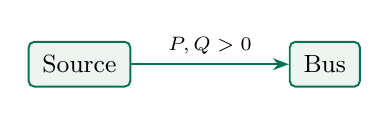
\begin{tikzpicture}
\node[box] (s) {Source};\node[box,right=2.0cm of s] (b) {Bus};
\draw[arrow] (s)--node[above,font=\scriptsize]{$P,Q>0$}(b);
\end{tikzpicture}\par
\medskip
{\small $P,Q$: net active/reactive power; $P_{\rm load},Q_{\rm load}$: demand; $p_{\rm PV},q_{\rm inv}$: inverter injections. Use one consistent power base.}
\column{.48\textwidth}
\uncover<2->{\VoltageIdea{The inverter absorbs reactive power}{$q_{\rm inv}<0$ increases net $Q$.}
\[
\Delta V\approx rP+xQ,\qquad V\approx V_s-\Delta V.
\]
\par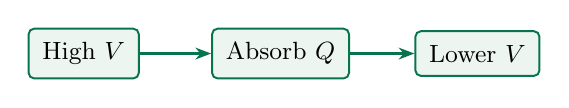
\begin{tikzpicture}[x=1cm,y=1cm]
\node[box] (v) at (0,0) {High $V$};
\node[box] (q) at (2.5,0) {Absorb $Q$};
\node[box] (w) at (5,0) {Lower $V$};
\draw[arrow] (v)--(q);\draw[arrow] (q)--(w);
\end{tikzpicture}\par
\medskip
{\small For positive line reactance $x$, more net reactive consumption increases the approximate drop.}}
\end{columns}
\uncover<3->{\VoltageIdea{Physical tradeoff}{Lower voltage can require more current. We must check both.}}

\Source{\href{https://arxiv.org/abs/1406.3054}{Gan \& Low: three-phase distribution optimization (2014)}; illustrative single-branch linearization, not a feeder measurement}
\Bridge{Can we calculate that voltage change with three numbers?}
\note{State both sign conventions explicitly. The distribution line sees net demand: positive P and Q mean consumption downstream. The inverter uses an injection convention, so positive reactive injection reduces net reactive demand, while absorption means a negative inverter reactive command and increases net Q. For a conventional line with positive resistance and reactance, increasing net reactive demand increases the approximate voltage drop. The voltage expression is a small-drop per-unit teaching approximation around nominal voltage, not the full three-phase model. Use the arrows to distinguish these quantities before introducing the actual fleet parameter b. The physical tradeoff is that reactive absorption may reduce high voltage while increasing the magnitude of current.}
\end{frame}

\begin{frame}[t]{A small calculation: reactive absorption lowers high voltage}
\label{f:V04}
\small

\begin{columns}[T]
\column{.40\textwidth}
\VoltageIdea{Illustrative single branch}{All quantities are per unit on consistent bases.}
\[
V_s=1.04,\quad r=0.02,\quad x=0.04,
\]
\[
P=-0.60.
\]
{\small Negative $P$ means net PV export. $Q$ is net reactive consumption. This is arithmetic for intuition, not output from the Greensboro model.}
\medskip
\par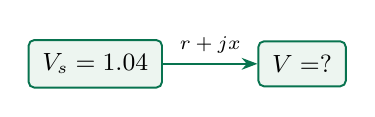
\begin{tikzpicture}
\node[box] (s) {$V_s=1.04$};\node[box,right=1.2cm of s] (b) {$V=?$};
\draw[arrow] (s)--node[above,font=\scriptsize]{$r+jx$}(b);
\end{tikzpicture}\par
\column{.57\textwidth}
\[
V\approx V_s-rP-xQ.
\]
\uncover<2->{\VoltageIdea{No reactive absorption: $Q=0$}{
$V\approx1.04-0.02(-0.60)=1.052$ p.u.\\
\textcolor{red}{Above the illustrative 1.05 p.u. upper bound.}}}
\medskip
\uncover<3->{\VoltageIdea{Absorb reactive power: $Q=0.20$}{
$V\approx1.04+0.012-0.008=1.044$ p.u.\\
\textcolor{teal}{The voltage now passes that bound.}}}
\end{columns}

\Source{Illustrative arithmetic using a linear voltage-drop approximation; \href{https://arxiv.org/abs/1406.3054}{Gan \& Low: three-phase distribution optimization (2014)}}
\Bridge{Does passing the voltage bound mean the action is acceptable?}
\note{Give the audience time to compute the first voltage before revealing it. The source voltage is 1.04 per unit, the line resistance and reactance are 0.02 and 0.04 per unit, and net active export is 0.60 per unit. With zero net reactive demand, the linear approximation predicts a voltage rise to 1.052. Adding 0.20 per unit of reactive absorption creates a drop that reduces the estimate to 1.044. The example intentionally uses round numbers and a single branch, so it is neither a calibrated feeder result nor a validation of the three-phase adapter. Ask which sign in the equation explains the change. The next slide checks the current consequence of the same action.}
\end{frame}

\begin{frame}[t]{Voltage passes, but current can still fail}
\label{f:V05}
\small

\[
I\approx\frac{\sqrt{P^2+Q^2}}{V_s},\qquad
V_{\max}=1.05,\quad I_{\max}=0.60\ {\rm p.u.}
\]
{\small $I$: approximate current magnitude; $P,Q$: net power; $V_s=1.04$ p.u. fixed reference. The limits are illustrative.}
\medskip
\begin{center}
\begin{tabular}{lrrrrl}
\hline
Action & $P$ & $Q$ & $V$ & $I$ & Checks\\\hline
PV export only & $-0.60$ & $0$ & $1.052$ & $0.577$ & \textcolor{red}{Voltage fails}\\
\uncover<2->{Add absorption} & \uncover<2->{$-0.60$} & \uncover<2->{$0.20$} & \uncover<2->{$1.044$} & \uncover<2->{$0.608$} & \uncover<2->{\textcolor{red}{Current fails}}\\
\uncover<3->{Also reduce export} & \uncover<3->{$-0.55$} & \uncover<3->{$0.20$} & \uncover<3->{$1.043$} & \uncover<3->{$0.563$} & \uncover<3->{\textcolor{teal}{Both pass}}\\\hline
\end{tabular}
\end{center}
\medskip
\Question{Which action would a voltage-only checker mistakenly accept?}
\uncover<3->{\VoltageIdea{Why we need optimization and verification}{Balance active power, reactive effort and every declared limit. A single improved metric is insufficient.}}

\Source{Explicitly illustrative per-unit arithmetic; no measured or simulated feeder result}
\Bridge{How can a planner coordinate these tradeoffs across several forecast steps?}
\note{Carry the previous voltage example forward without changing its assumptions. The approximate current uses apparent-power magnitude divided by the fixed source-voltage reference. PV export alone gives acceptable current but excessive voltage. Reactive absorption fixes the voltage while increasing current slightly beyond the illustrative limit. Reducing the magnitude of active export then makes both checks pass in this approximation. The three rows isolate the tradeoff and explain why a good voltage result is not enough. All values are rounded and belong only to this single-branch arithmetic example. They are not the tutorial's actual MPC or SAC commands. Ask participants to name any additional checks still missing, including inverter capability and the validity of the model itself.}
\end{frame}

\begin{frame}[t]{The five stages turn an action into reviewable evidence}
\label{f:V06}
\small

\begin{center}
\par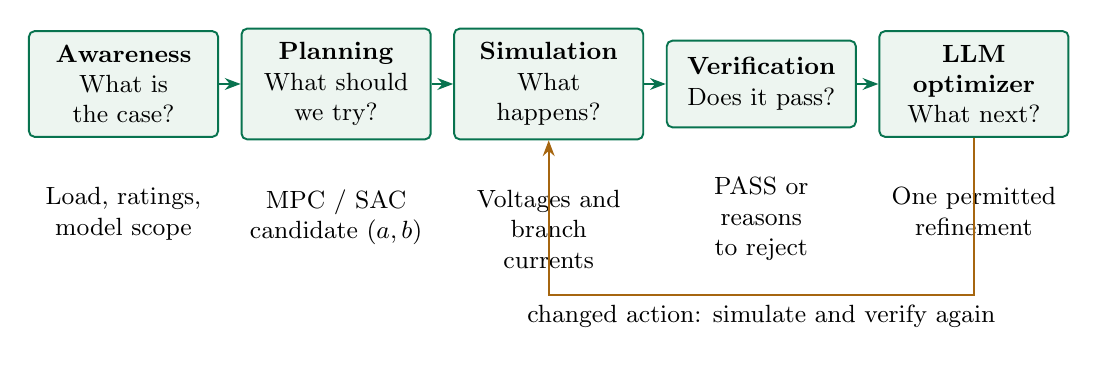
\begin{tikzpicture}[x=1cm,y=1cm]
\node[box,text width=2.05cm,minimum height=1.1cm] (a) at (0,0) {\textbf{Awareness}\\What is the case?};
\node[box,text width=2.05cm,minimum height=1.1cm] (p) at (2.7,0) {\textbf{Planning}\\What should we try?};
\node[box,text width=2.05cm,minimum height=1.1cm] (s) at (5.4,0) {\textbf{Simulation}\\What happens?};
\node[box,text width=2.05cm,minimum height=1.1cm] (v) at (8.1,0) {\textbf{Verification}\\Does it pass?};
\node[box,text width=2.05cm,minimum height=1.1cm] (o) at (10.8,0) {\textbf{LLM\\optimizer}\\What next?};
\draw[arrow] (a)--(p);\draw[arrow] (p)--(s);\draw[arrow] (s)--(v);\draw[arrow] (v)--(o);
\uncover<2->{\node[below=5mm of a,text width=2.2cm,align=center,font=\small] {Load, ratings,\\model scope};
\node[below=5mm of p,text width=2.2cm,align=center,font=\small] {MPC / SAC\\candidate $(a,b)$};
\node[below=5mm of s,text width=2.2cm,align=center,font=\small] {Voltages and\\branch currents};
\node[below=5mm of v,text width=2.2cm,align=center,font=\small] {PASS or reasons\\to reject};
\node[below=5mm of o,text width=2.2cm,align=center,font=\small] {One permitted\\refinement};}
\uncover<3->{\draw[arrow,draw=amber] (o.south) -- ++(0,-2.0) -| node[pos=.25,below,font=\small]{changed action: simulate and verify again} (s.south);}
\end{tikzpicture}\par
\end{center}
\VoltageIdea{The lesson from the arithmetic}{The optimizer may suggest reducing export. The numerical checker must establish whether that new command meets the declared limits.}

\Source{Executed \texttt{Classroom\_Labs.ipynb}; \texttt{src/classroom\_labs.py}; five-stage proposal architecture}
\Bridge{What does the model-based planner calculate?}
\note{Connect each stage to the physical tradeoff just calculated. Awareness establishes the source conditions, ratings, model scope and permitted actions. Planning proposes a command, using the appropriate numerical method. Simulation computes its consequences, while verification decides whether those consequences satisfy the contract. The language optimizer can select a permitted next trial, but the modified command has to return to the numerical stages. The actual tutorial uses MPC and SAC as candidate generators and model-specific power-flow adapters for checking. It does not require an LLM call in every stage. Deterministic computation remains essential. Ask learners to identify which stages repeat after changing only reactive absorption, and which evidence must be replaced.}
\end{frame}

\begin{frame}[t]{MPC uses a forecast, then commits only the first move}
\label{f:V07}
\small

\begin{center}
\par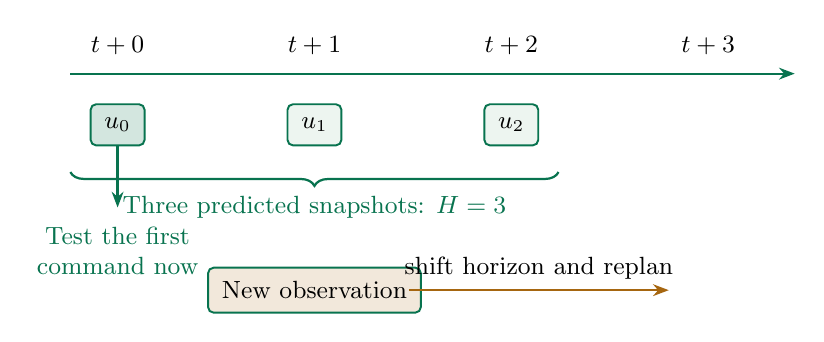
\begin{tikzpicture}[x=1cm,y=1cm]
\foreach \x/\t in {0/0,2.5/1,5/2,7.5/3} {\node[font=\small] at (\x,.8) {$t+\t$};}
\draw[arrow] (-.6,.45)--(8.6,.45);
\node[box,fill=teal!18] (u0) at (0,-.2) {$u_0$};
\node[box] at (2.5,-.2) {$u_1$};\node[box] at (5,-.2) {$u_2$};
\draw[decorate,decoration={brace,mirror,amplitude=5pt},thick,teal] (-.6,-.8)--node[below=5pt,font=\small]{Three predicted snapshots: $H=3$}(5.6,-.8);
\uncover<2->{\node[font=\small,text=teal,align=center] at (0,-1.8) {Test the first\\command now};
\draw[arrow] (u0)--(0,-1.25);
\node[box,fill=amber!15] at (2.5,-2.3) {New observation};
\draw[arrow,draw=amber] (3.7,-2.3)--node[above,font=\small]{shift horizon and replan}(7,-2.3);}
\end{tikzpicture}\par
\end{center}
\[
\min_{u_{0:H-1}}\sum_{k=0}^{H-1}\gamma^k\ell(x_k,u_k)
\quad\text{s.t. prediction model and operating limits.}
\]
{\small $u_k$: control; $x_k$: predicted state; $H$: horizon; $\gamma=0.98$: discount; $\ell$: one-step cost. Here: algebraic power-flow snapshots linked by command-movement cost.}

\Source{\href{https://sites.engineering.ucsb.edu/~jbraw/mpc/}{Rawlings, Mayne \& Diehl: MPC (2017)}}
\Bridge{Which preferences should one command optimize?}
\note{Build the timeline one element at a time. The central concept is repeated optimization using new information, rather than executing an entire old plan without revision. The generic MPC framework can contain dynamics and long horizons. This tutorial implements H=3 quasi-static power-flow snapshots, linked by a penalty on command movement. It returns the first proposed control for a fresh check. It does not demonstrate transient stability or a complete closed-loop field rollout. Ask learners why a new forecast could change the later controls and why only the first control is considered now. The next slide formalizes these ideas without hiding the difference between general MPC and the implemented approximation.}
\end{frame}

\begin{frame}[t]{The objective makes engineering preferences explicit}
\label{f:V08}
\small

\begin{columns}[T]
\column{.34\textwidth}
\VoltageIdea{One fleet command}{$u=(a,b)$ is dimensionless.}
\[
p_i=aS_i,\qquad q_i=bS_i.
\]
{\small $S_i$: inverter rating (kVA); $p_i$: active power (kW); $q_i$: reactive injection (kvar).\\[1mm]
$b<0$ means absorption. $u_{\rm prev}$ is the previous command.}
\column{.63\textwidth}
\begin{align*}
\ell={}&\underbrace{(1-a)^2}_{\text{unused active capability}}
+\underbrace{0.05b^2}_{\text{reactive effort}}\\
&+\underbrace{10\,\mathrm{mean}[(V-1.01)^2]}_{\text{voltage deviation}}\\
&+\underbrace{0.05\|u-u_{\rm prev}\|_2^2}_{\text{command movement}}.
\end{align*}
{\small $V$: modeled voltage magnitudes (p.u.); $\ell$: dimensionless weighted teaching cost.}
\end{columns}
\uncover<2->{\Question{If $|b|$ decreases, which cost term certainly decreases?}
\Answer{Reactive effort. The voltage and movement terms can still worsen.}}

\Source{Recorded \texttt{LLM\_Response\_Selection.ipynb}; raw calls in \texttt{results/ensemble\_voltage\_pilot/}}
\Bridge{Which physical limits can overrule a low cost?}
\note{Reveal the cost one term at a time and ask learners to name the engineering preference represented by each term. The first term discourages curtailment under the declared availability assumption. The second discourages reactive effort. The third measures mean squared voltage deviation over the modeled bus-phase set. The fourth penalizes command movement. All weights are teaching design choices, not universal operating preferences. Reducing the magnitude of b certainly reduces the reactive-effort term, but can alter voltages, movement and feasibility. The objective is evaluated for the current step in the reported comparisons. A better objective alone establishes neither stability nor a safe recommendation outside the modeled contract.}
\end{frame}

\begin{frame}[t]{The admissible region is a gate, not another preference}
\label{f:V09}
\small

\begin{columns}[T]
\column{.39\textwidth}
\par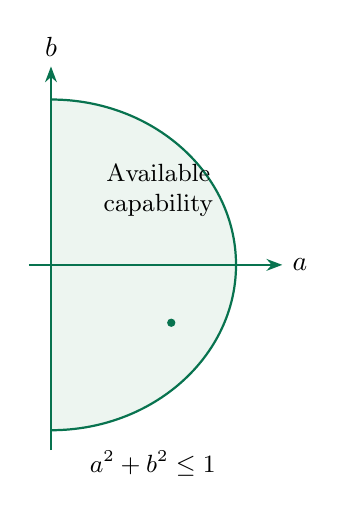
\begin{tikzpicture}[x=2.35cm,y=2.1cm]
\fill[pale] (0,0)--(0,-1) arc[start angle=-90,end angle=90,radius=1]--cycle;
\draw[thick,teal] (0,-1) arc[start angle=-90,end angle=90,radius=1];
\draw[arrow] (-.12,0)--(1.25,0) node[right] {$a$};
\draw[arrow] (0,-1.12)--(0,1.2) node[above] {$b$};
\fill[teal] (.65,-.35) circle(1.5pt);
\node[font=\small,align=center] at (.58,.45) {Available\\capability};
\node[font=\small] at (.55,-1.2) {$a^2+b^2\le1$};
\end{tikzpicture}\par
\column{.58\textwidth}
\VoltageIdea{Network limits}{
$V_{\min}\le |V_i|\le V_{\max},\quad |I_e|\le I_e^{\max}$.}
{\small $V_i$: bus-phase voltage; $I_e$: branch current; bounds belong to the request.}
\medskip
\VoltageIdea{Inverter limits}{
$p_i^2+q_i^2\le S_i^2$ gives the capability circle; $0\le a\le1$ and declared bounds on $b$ also apply.}
\medskip
\uncover<2->{\VoltageIdea{Evidence limits}{Finite inputs, solver completion, dispatch tracking and matching request/candidate/model identifiers.}}
\end{columns}


\Source{\href{https://sites.engineering.ucsb.edu/~jbraw/mpc/}{Rawlings, Mayne \& Diehl: MPC (2017)}; Recorded \texttt{LLM\_Response\_Selection.ipynb}; raw calls in \texttt{results/ensemble\_voltage\_pilot/}}
\Bridge{Which constraints are visible to each power-flow model?}
\note{Draw the inverter capability circle while revealing the network bounds. The circle follows from the apparent-power limit after dividing by the squared rating. The planner uses local sensitivities and a conservative capability polygon; the final proposal still returns to a numerical model for checking. Distinguish a solver returning normally, a good cost and a feasible candidate. These are separate observations. Evidence validity also requires matching case, candidate and model identifiers, so results from a previous setting cannot be attached to a new one. Ask whether three language models agreeing can make a branch overcurrent acceptable. The answer locates the engineering gate above preference selection.}
\end{frame}

\begin{frame}[t]{The two models cover different parts of the feeder}
\label{f:V10}
\small

\begin{center}
\par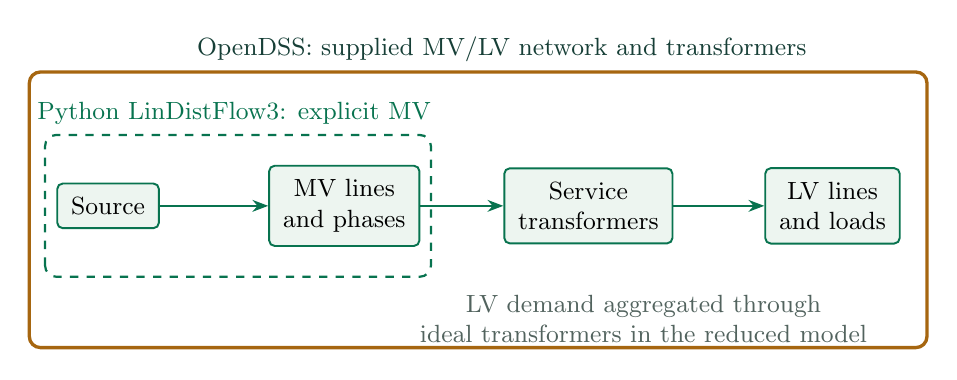
\begin{tikzpicture}[x=1cm,y=1cm]
\node[box] (src) at (0,0) {Source};
\node[box] (mv) at (3,0) {MV lines\\and phases};
\node[box] (tx) at (6.1,0) {Service\\transformers};
\node[box] (lv) at (9.2,0) {LV lines\\and loads};
\draw[arrow] (src)--(mv);\draw[arrow] (mv)--(tx);\draw[arrow] (tx)--(lv);
\draw[rounded corners,teal,thick,dashed] (-.8,-.9) rectangle (4.1,.9);
\node[above,font=\small,text=teal] at (1.6,.9) {Python LinDistFlow3: explicit MV};
\node[below,font=\small,align=center,text=slate] at (6.8,-1) {LV demand aggregated through\\ideal transformers in the reduced model};
\uncover<2->{\draw[rounded corners,amber,very thick] (-1,-1.8) rectangle (10.4,1.7);
\node[above,font=\small,text=navy] at (5,1.7) {OpenDSS: supplied MV/LV network and transformers};}
\end{tikzpicture}\par
\end{center}
\begin{columns}[T]
\column{.48\textwidth}\VoltageIdea{Reduced-model PASS}{Within the MV-only approximation and its checked limits.}
\column{.48\textwidth}\VoltageIdea{Full-model PASS}{Within the broader unbalanced snapshot contract.}
\end{columns}
\uncover<3->{\textbf{Comparison boundary:} equations \emph{and} constraint coverage change; this is not an accuracy-only test.}

\Source{\href{https://arxiv.org/abs/1406.3054}{Gan \& Low: three-phase distribution optimization (2014)}; \href{https://opendss.epri.com/}{EPRI OpenDSS documentation}}
\Bridge{What is retained in the transparent three-phase approximation?}
\note{Keep two model cards visible while adding their coverage. Python LinDistFlow3 implements a coupled three-phase linear approximation on the MV network. Its ideal aggregation does not expose LV voltages or transformer thermal constraints. OpenDSS solves the supplied unbalanced MV/LV power-flow model. Both are useful for their declared purpose, but their PASS labels answer different questions. This experiment changes both model equations and coverage. It therefore cannot isolate a pure approximation-error effect. Even the voltage term in the objective is aggregated over different modeled sets. Ask learners which additional limits could fail when the same command is sent to the broader model.}
\end{frame}

\begin{frame}[t]{Three-phase LinDistFlow keeps mutual phase coupling}
\label{f:V11}
\small

\begin{columns}[T]
\column{.32\textwidth}
\par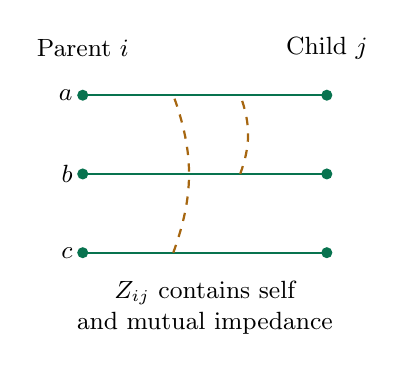
\begin{tikzpicture}[x=1cm,y=1cm]
\foreach \y/\ph in {1/a,0/b,-1/c}{
\fill[teal] (0,\y) circle(2pt);\fill[teal] (3.1,\y) circle(2pt);
\draw[thick,teal] (0,\y)--(3.1,\y);
\node[left,font=\small] at (0,\y) {$\ph$};}
\draw[amber,thick,dashed] (1.15,-1) to[bend right=20] (1.15,1);
\draw[amber,thick,dashed] (2,0) to[bend right=20] (2,1);
\node[font=\small] at (0,1.6) {Parent $i$};
\node[font=\small] at (3.1,1.6) {Child $j$};
\node[font=\small,align=center] at (1.55,-1.7) {$Z_{ij}$ contains self\\and mutual impedance};
\end{tikzpicture}\par
\column{.65\textwidth}
\[
\mathbf w_j=\mathbf w_i-
2\operatorname{Re}\!\left[
\overline{\beta}\odot
\left(Z_{ij}(\beta\odot\overline{\mathbf S}_{ij})\right)
\right].
\]
{\small
$\mathbf w_i,\mathbf w_j$: squared phase voltages (V$^2$);\\
$Z_{ij}$: coupled phase-impedance matrix ($\Omega$);\\
$\mathbf S_{ij}$: downstream phase powers (VA);\\
$\beta=(1,e^{-{\rm j}2\pi/3},e^{-{\rm j}4\pi/3})$: nominal phase ratios.\\
$\overline{\cdot}$: conjugate; $\odot$: entrywise multiplication; $\operatorname{Re}$: real part; $\mathrm{j}^2=-1$.}
\uncover<2->{\medskip\VoltageIdea{The approximation}{Nominal angle ratios and lossless branch balances. Current uses a fixed 1.03-p.u. reference; losses are diagnostic.}}
\end{columns}

\Source{\href{https://arxiv.org/abs/1406.3054}{Gan \& Low: three-phase distribution optimization (2014)}; exact adapter: \texttt{src/lindistflow3.py}}
\Bridge{How does a learned actor produce a candidate without solving this optimization now?}
\note{Start from the parent and child buses, then reveal the voltage-drop term. The equation matches the fixed phase-ratio closure used by the Python adapter. The matrix Z contains mutual phase coupling, so this is not a single-phase equivalent. The beta vector encodes nominal phase relationships, overbars denote complex conjugation, the circle-like multiplication symbol means entrywise multiplication and Re extracts the real component. Branch powers are in VA and squared voltages in volts squared. The imaginary unit in the exponent is distinct from a bus index. Currents use fixed source-reference phasors at 1.03 p.u.; small-loss assumptions are not certified error bounds. The full limitations remain in the handout.}
\end{frame}

\begin{frame}[t]{SAC learns a continuous action rule; checking remains separate}
\label{f:V12}
\small

\begin{center}
\par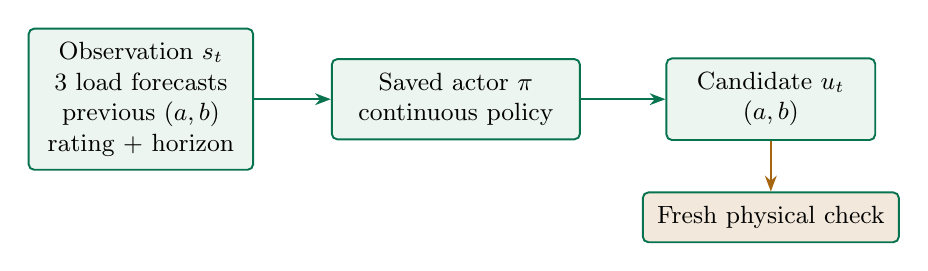
\begin{tikzpicture}[x=1cm,y=1cm]
\node[box,text width=2.5cm] (s) at (0,0) {Observation $s_t$\\3 load forecasts\\previous $(a,b)$\\rating + horizon};
\node[box,text width=2.8cm] (a) at (4,0) {Saved actor $\pi$\\continuous policy};
\node[box,text width=2.3cm] (u) at (8,0) {Candidate $u_t$\\$(a,b)$};
\draw[arrow] (s)--(a);\draw[arrow] (a)--(u);
\uncover<2->{\node[box,fill=amber!15,text width=2.9cm] (g) at (8,-1.5) {Fresh physical check};
\draw[arrow,draw=amber] (u)--(g);}
\end{tikzpicture}\par
\end{center}
\[
\max_\pi \mathbb E\!\left[
\sum_{t\ge0}\gamma^t
\left\{\underbrace{r(s_t,u_t)}_{\text{task reward}}+
\underbrace{\alpha\,\mathcal H(\pi(\cdot\mid s_t))}_{\text{exploration during learning}}\right\}\right].
\]
{\small $s_t$: observation; $u_t$: action; $r$: reward; $\pi$: policy; $\mathcal H$: entropy; $\alpha$: exploration weight; $\gamma$: discount; $t$: time step; $\mathbb E$: expectation over trajectories.}
\uncover<3->{\textbf{Executed: SAC.}\quad PPO is a continuous-action alternative discussed here, not another trained result.}

\Source{\href{https://proceedings.mlr.press/v80/haarnoja18b.html}{Haarnoja et al.: SAC, ICML 2018}; \href{https://arxiv.org/abs/1707.06347}{Schulman et al.: PPO (2017)}}
\Bridge{What computation produced the saved actor?}
\note{Use this equation to explain the purpose of SAC rather than derive every update rule. The actor is a probability distribution over continuous actions. The actual saved actor receives three forecast load factors, the previous two-number command, the rating fraction and the remaining-horizon fraction. The task reward expresses operational preferences and penalties, while entropy encourages broader exploration during training. Alpha controls that tradeoff and gamma discounts future rewards. Training and inference are different phases: the classroom loads saved weights and computes a new action for the current observation. It does not retrain the policy. Even a strong reward penalty for violations can leave unsafe actions under distribution shift. This is why the actor is a candidate generator within the workflow, followed by simulation and a hard acceptance gate.}
\end{frame}

\begin{frame}[t]{Training provenance prevents a misleading speed claim}
\label{f:V13}
\small

\begin{center}
\par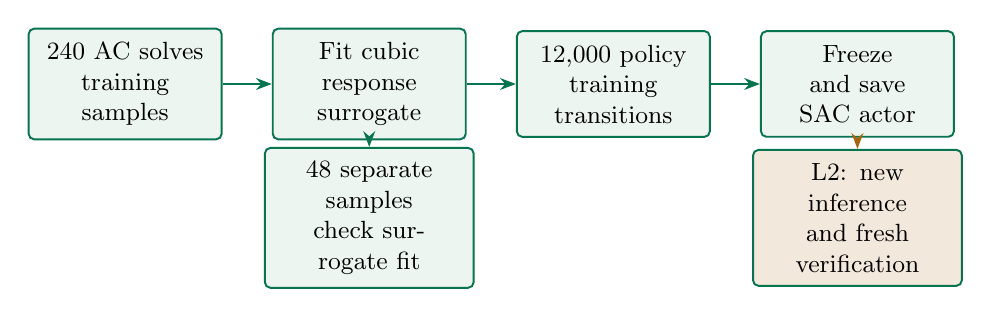
\begin{tikzpicture}[x=1cm,y=1cm]
\node[box,text width=2.1cm,minimum height=1.1cm] (ac) at (0,0) {240 AC solves\\training samples};
\node[box,text width=2.1cm,minimum height=1.1cm] (fit) at (3.1,0) {Fit cubic\\response surrogate};
\node[box,text width=2.1cm,minimum height=1.1cm] (learn) at (6.2,0) {12,000 policy\\training transitions};
\node[box,text width=2.1cm,minimum height=1.1cm] (actor) at (9.3,0) {Freeze and save\\SAC actor};
\draw[arrow] (ac)--(fit);\draw[arrow] (fit)--(learn);\draw[arrow] (learn)--(actor);
\uncover<2->{\node[box,text width=2.3cm] (val) at (3.1,-1.7) {48 separate samples\\check surrogate fit};
\draw[arrow] (fit)--(val);
\node[box,fill=amber!15,text width=2.3cm] (now) at (9.3,-1.7) {L2: new inference\\and fresh verification};
\draw[arrow,draw=amber] (actor)--(now);}
\end{tikzpicture}\par
\end{center}
\begin{columns}[T]
\column{.48\textwidth}\VoltageIdea{What the count means}{12,000 transitions on the fitted surrogate, not 12,000 full AC solves.}
\column{.48\textwidth}\VoltageIdea{What transfer means}{A new load or rating condition can challenge the frozen actor; L2 does not retrain it.}
\end{columns}

\Source{\href{https://proceedings.mlr.press/v80/haarnoja18b.html}{Haarnoja et al.: SAC, ICML 2018}; executed training artifact: \texttt{Continuous\_SAC\_Training.ipynb}}
\Bridge{Which operations will the classroom cell recompute?}
\note{Animate a pipeline from AC samples to surrogate fitting to policy training to the saved actor. The 12,000 transitions are not 12,000 OpenDSS solves. This distinction matters for reproducibility and for reporting computational cost. The fit-validation samples assess the surrogate, not all aspects of policy robustness. New classroom scenarios can alter demand or current-rating conditions, creating a transfer problem for the frozen actor. A quick inference time therefore says little about total development cost or reliability under shift. Ask learners what evidence they would request before trusting the actor beyond this fixture. Possible answers include separate policy test cases, out-of-distribution conditions, constraint failures and an appropriate deterministic baseline.}
\end{frame}

\begin{frame}[t]{L2 recomputes both proposals under one declared scenario}
\label{f:V14}
\small

\Checkpoint{L2}{Fresh MPC solve + saved SAC inference + fresh numerical checks.}
\begin{columns}[T]
\column{.57\textwidth}
\lstinputlisting[style=python,firstline=1,lastline=7]{snippets/L2.py}
\column{.40\textwidth}
\par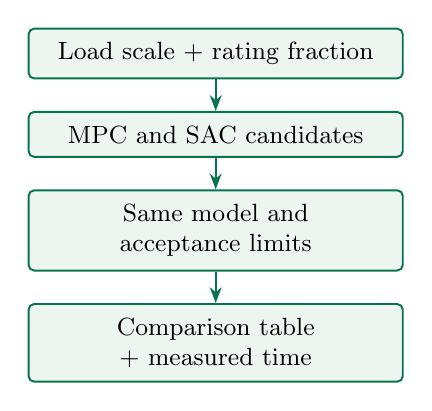
\begin{tikzpicture}[node distance=4mm]
\node[box,text width=4.4cm] (r) {Load scale + rating fraction};
\node[box,text width=4.4cm,below=of r] (p) {MPC and SAC candidates};
\node[box,text width=4.4cm,below=of p] (v) {Same model and acceptance limits};
\node[box,text width=4.4cm,below=of v] (t) {Comparison table + measured time};
\draw[arrow] (r)--(p);\draw[arrow] (p)--(v);\draw[arrow] (v)--(t);
\end{tikzpicture}\par
\end{columns}
\uncover<2->{\VoltageIdea{Read the timer correctly}{It encloses the helper call: planning, actor inference and checks. It is not isolated SAC inference latency.}}

\Source{Executed \texttt{Classroom\_Labs.ipynb}; \texttt{src/classroom\_labs.py}}
\Bridge{What do you predict will change when demand changes?}
\note{Walk through the exact first seven lines of L2. LOAD\_SCALE and RATING\_FRACTION are the two visible scenario controls. The helper performs a fresh MPC calculation, new saved-actor inference and new numerical checks. The timer encloses the helper call, so it measures more than policy inference alone. The returned table is the place to compare feasibility and cost before looking at the plot. Keep the original default outputs as a reference, then make one change at a time. The later L3 response pool belongs to a different archived original context; rerunning L2 does not regenerate those LLM responses. This boundary must stay explicit during the exercise.}
\end{frame}

\begin{frame}[t]{Lab: predict, change demand, then explain the response}
\label{f:V15}
\small

\Checkpoint{L2}{Seven minutes in pairs. Run the full cell, not only this excerpt.}
\begin{columns}[T]
\column{.43\textwidth}
\lstinputlisting[style=python,firstline=1,lastline=4]{snippets/L2.py}
\begin{enumerate}
\item Predict the effect of higher demand.
\item Run the default case.
\item Change only \texttt{LOAD\_SCALE}; rerun L2.
\item Explain the limiting margin, not just the winner.
\end{enumerate}
\column{.54\textwidth}
\begin{center}
\begin{tabular}{p{2.2cm}p{1.5cm}p{1.5cm}}
\hline
Record & Default & Changed\\\hline
Feasible? & \rule{1.1cm}{.3pt} & \rule{1.1cm}{.3pt}\\[2mm]
Objective & \rule{1.1cm}{.3pt} & \rule{1.1cm}{.3pt}\\[2mm]
Voltage margin & \rule{1.1cm}{.3pt} & \rule{1.1cm}{.3pt}\\[2mm]
Current margin & \rule{1.1cm}{.3pt} & \rule{1.1cm}{.3pt}\\\hline
\end{tabular}
\end{center}
\uncover<2->{\Question{Must higher demand increase PV curtailment?}
\Answer{No. Voltage and current constraints can move in different directions.}}
\end{columns}

\Source{Executed \texttt{Classroom\_Labs.ipynb}; \texttt{src/classroom\_labs.py}}
\Bridge{Which plotted margin supports your explanation?}
\note{Allow seven minutes and keep this slide visible while participants work. One learner predicts and one operates the notebook, then they exchange roles. First record the default results. Next choose a modest changed load multiplier and predict how PV participation, reactive support or curtailment might respond. Run the full L2 cell and compare the same acceptance metrics. Students should explain a result using a numerical margin rather than a general claim about AI. If setup fails, use the executed notebook output to complete the prediction and interpretation tasks. Do not modify unrelated cells or imply that the archived LLM pool has changed. Finish by collecting one surprising observation from the room.}
\end{frame}

\begin{frame}[t]{Inspect the physical margins before ranking the controllers}
\label{f:V16}
\small

\begin{center}
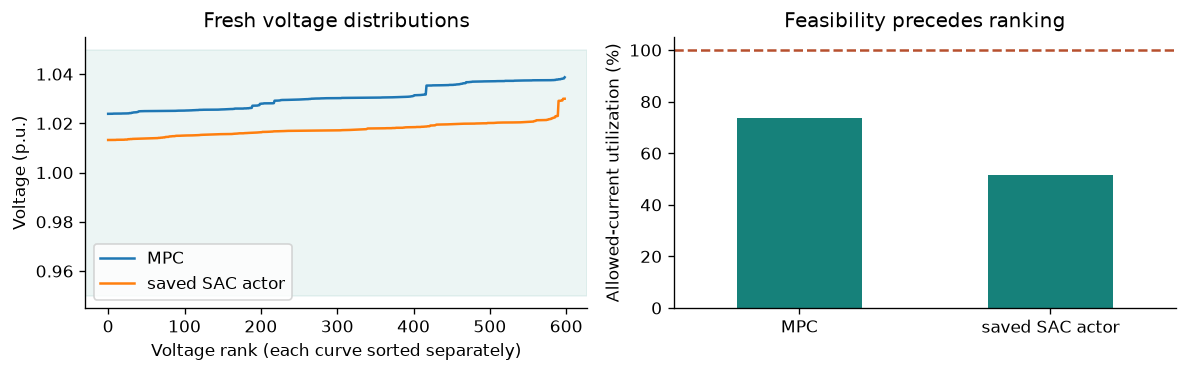
\includegraphics[width=.92\linewidth,height=3.25cm,keepaspectratio]{figures/classroom_voltage.png}
\end{center}
\begin{columns}[T]
\column{.48\textwidth}
\begin{tabular}{lrr}
\hline
Fresh L2 default & $J$ & MV gate\\\hline
MPC & 0.031104 & PASS\\
Saved SAC actor & 0.436428 & PASS\\\hline
\end{tabular}
\column{.48\textwidth}
{\small $J$: current-step teaching cost. Both actions pass this reduced-model contract. The voltage curves are sorted separately: equal rank is not equal bus identity.}
\end{columns}
\uncover<2->{\VoltageIdea{Attribute the result correctly}{The cost gap is a controller result. It does not, by itself, measure the benefit of agent orchestration.}}

\Source{Executed \texttt{Classroom\_Labs.ipynb}; \texttt{src/classroom\_labs.py}}
\Bridge{What can a language model add after numerical evidence already exists?}
\note{Use the actual executed L2 figure. The displayed default costs are rounded for teaching: MPC is approximately 0.031104 and SAC 0.436428, with both feasible under the reduced-model contract. The voltage curves are sorted separately, so matching positions are ranks rather than the same physical bus. The current-utilization plot reports the most heavily used allowed current bound. Ask participants to identify the evidence for feasibility before comparing objective values. A cost gap here is a controller result, not automatically an advantage of the multi-agent architecture. Students with changed load settings should report their own values and avoid mixing them with this original reference output.}
\end{frame}

\begin{frame}[t]{L3 opens a different, explicitly archived context}
\label{f:V17}
\small

\Checkpoint{L3}{Inspect original \texttt{test\_01}; these are actual recorded model responses.}
\begin{columns}[T]
\column{.53\textwidth}
\lstinputlisting[style=python,firstline=1,lastline=8]{snippets/L3.py}
\column{.44\textwidth}
\par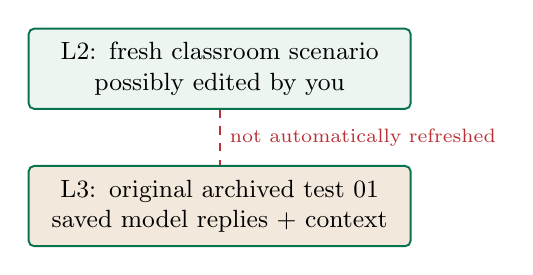
\begin{tikzpicture}[node distance=7mm]
\node[box,text width=4.5cm] (live) {L2: fresh classroom scenario\\possibly edited by you};
\node[box,fill=amber!15,text width=4.5cm,below=of live] (arc) {L3: original archived test 01\\saved model replies + context};
\draw[red,thick,dashed] (live.south)--node[right,font=\scriptsize,text=red]{not automatically refreshed}(arc.north);
\end{tikzpicture}\par
\medskip
\uncover<2->{\VoltageIdea{Read the provenance}{
\texttt{reason}: exact public response.\\
\texttt{seconds}: recorded call time.\\
Printing the table makes no new LLM call.}}
\end{columns}

\Source{Executed \texttt{Classroom\_Labs.ipynb}; \texttt{src/classroom\_labs.py}; Recorded \texttt{LLM\_Response\_Selection.ipynb}; raw calls in \texttt{results/ensemble\_voltage\_pilot/}}
\Bridge{Do the actual explanations support the physical claims they make?}
\note{Explain why this cell is reproducible without contacting a local model. It loads an archived response pool from original test\_01, displays each exact public response and reports how the structured proposals were canonicalized. The seconds column contains recorded call durations, not the time required to print the table. The original test context is not identical to L2's default rating fraction, and certainly not to a student-modified L2 scenario. This cell therefore teaches inspection and evidence attribution. It does not supply new context-matched recommendations for the latest classroom perturbation. Ask learners to find a claim in a reason that is supported by the numeric evidence and one that still requires testing.}
\end{frame}

\begin{frame}[t]{Read the actual replies, then challenge their claims}
\label{f:V18}
\small

{\small Exact public excerpts, archived original test 01. Llama is the model family; Ollama is the local runtime.}
\medskip
\begin{columns}[T]
\column{.32\textwidth}
\VoltageIdea{Llama 3.1 8B \quad 1.867 s}{Trial: increase $a$ by 0.0025.}
{\small\itshape Increasing active participation by 0.0025 may help reduce curtailment and improve the overall performance.}
\column{.32\textwidth}
\VoltageIdea{Llama 3.2 3B \quad 0.905 s}{Trial: reduce $|b|$ by 10\%.}
{\small\itshape Reducing reactive effort magnitude by ten percent may help improve the overall system performance and reduce curtailment}
\column{.32\textwidth}
\VoltageIdea{Qwen 2.5 7B \quad 1.844 s}{Trial: reduce $|b|$ by 10\%.}
{\small\itshape may help improve voltage stability without significantly degrading active power performance}
\end{columns}
\medskip
\uncover<2->{\Question{Which phrases need evidence beyond a plausible explanation?}}
\uncover<3->{\begin{columns}[T]
\column{.48\textwidth}\VoltageIdea{Reactive effort $\ne$ curtailment}{Reducing $|b|$ does not itself prove higher active generation.}
\column{.48\textwidth}\VoltageIdea{Snapshot $\ne$ stability proof}{Steady-state power flow does not establish voltage stability.}
\end{columns}}

\Source{Recorded \texttt{LLM\_Response\_Selection.ipynb}; raw calls in \texttt{results/ensemble\_voltage\_pilot/}}
\Bridge{How do we compare three replies as physical actions?}
\note{These times and choices come from the recorded response-selection pilot. Llama 3.1 suggested increasing active participation to reduce curtailment. Llama 3.2 described reducing reactive effort and also mentioned reducing curtailment, a causal connection that its text alone does not establish. Qwen used the phrase voltage stability, which is unsupported by these steady-state tests. Present the excerpts as public rationales, not access to private model reasoning. Llama names the model family; Ollama is the local runtime that served it. Have the audience annotate the difference between a permitted operation and a justified physical claim. The next step converts prose-backed choices into reproducible physical candidates.}
\end{frame}

\begin{frame}[t]{Canonicalize actions before counting votes}
\label{f:V19}
\small

\begin{center}
\par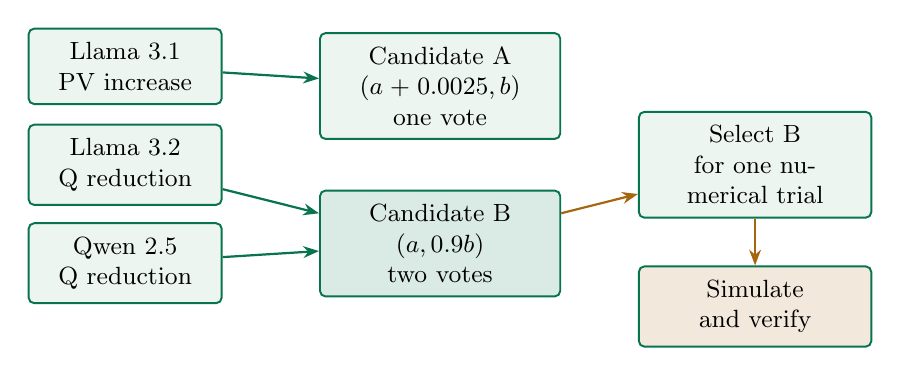
\begin{tikzpicture}[x=1cm,y=1cm]
\node[box,text width=2.1cm] (l1) at (0,1.25) {Llama 3.1\\PV increase};
\node[box,text width=2.1cm] (l2) at (0,0) {Llama 3.2\\Q reduction};
\node[box,text width=2.1cm] (qw) at (0,-1.25) {Qwen 2.5\\Q reduction};
\node[box,text width=2.7cm] (pv) at (4,1) {Candidate A\\$(a+0.0025,b)$\\one vote};
\node[box,fill=teal!15,text width=2.7cm] (qr) at (4,-1) {Candidate B\\$(a,0.9b)$\\two votes};
\draw[arrow] (l1)--(pv);\draw[arrow] (l2)--(qr);\draw[arrow] (qw)--(qr);
\uncover<2->{\node[box,text width=2.6cm] (sel) at (8,0) {Select B\\for one numerical trial};
\draw[arrow,draw=amber] (qr)--(sel);}
\uncover<3->{\node[box,fill=amber!15,text width=2.6cm] (check) at (8,-1.8) {Simulate and verify};
\draw[arrow,draw=amber] (sel)--(check);}
\end{tikzpicture}\par
\end{center}
{\small $a,b$: incumbent fleet command. Tool name and parameters identify the same physical operation; prose style does not create a new action.}
\VoltageIdea{A majority is a selection rule}{Correlated language models can share an error. Agreement is not a calibrated probability of safety.}

\Source{Recorded \texttt{LLM\_Response\_Selection.ipynb}; raw calls in \texttt{results/ensemble\_voltage\_pilot/}}
\Bridge{Can experience improve the choice of which candidate to test?}
\note{Animate three response cards merging into two physical-candidate cards. Two different descriptions of the same command must not count as two distinct control actions. Canonical identifiers depend on the tool and parameters rather than rhetorical style. In original test\_01, two models propose the same reactive reduction and one proposes a PV increase, so the majority chooses the reactive trial. A predetermined hash tie-break makes ties reproducible; it is not an engineering preference. Agreement is also not a calibrated safety probability because models can share mistaken assumptions. A changed command returns to the numerical stages. Ask what should happen if the majority-selected trial fails a current constraint.}
\end{frame}

\begin{frame}[t]{LinUCB learns which proposed operation is worth testing}
\label{f:V20}
\small

\begin{columns}[T]
\column{.40\textwidth}
\par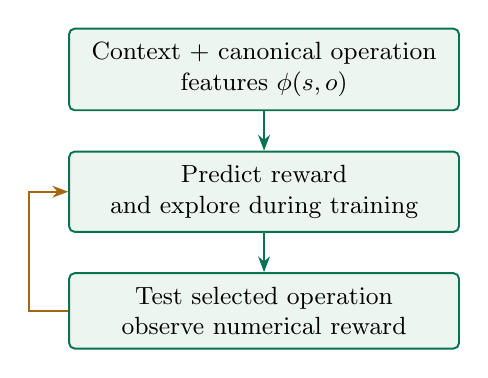
\begin{tikzpicture}[node distance=5mm]
\node[box,text width=4.6cm] (x) {Context + canonical operation\\features $\phi(s,o)$};
\node[box,text width=4.6cm,below=of x] (q) {Predict reward\\and explore during training};
\node[box,text width=4.6cm,below=of q] (r) {Test selected operation\\observe numerical reward};
\draw[arrow] (x)--(q);\draw[arrow] (q)--(r);
\uncover<2->{\draw[arrow,draw=amber] (r.west)--++(-.5,0)|- (q.west);}
\end{tikzpicture}\par
\column{.57\textwidth}
\begin{align*}
q(o\mid s)={}&
\underbrace{\theta^\top\phi(s,o)}_{\text{predicted reward}}\\
&+\underbrace{\beta\sqrt{\phi(s,o)^\top A^{-1}\phi(s,o)}}_{\text{training exploration bonus}},\\
o^*={}&\arg\max_o q(o\mid s).
\end{align*}
{\small $s$: evidence context; $o$: canonical operation; $\phi$: features; $\theta$: learned coefficients; $A$: regularized feature information; $\beta$: exploration weight; $q$: score; $o^*$: selected operation.}
\end{columns}
\uncover<3->{\VoltageIdea{Frozen classroom evaluation}{Use predicted reward only, with no updates. All LLM replies already exist: this learner does not choose which model to call or train LLM weights.}}

\Source{\href{https://arxiv.org/abs/1003.0146}{Li et al.: LinUCB, WWW 2010}; Recorded \texttt{LLM\_Response\_Selection.ipynb}; raw calls in \texttt{results/ensemble\_voltage\_pilot/}}
\Bridge{What should happen when a high predicted reward fails the physical gate?}
\note{Explain select, observe and update before revealing the formula. The feature vector represents the known context and a canonical operation, including vote-related information. Theta stores learned reward coefficients; A stores regularized feature information. During training, beta controls an uncertainty bonus. After a trial, selected feedback updates the reward model. The classroom evaluation freezes these parameters and uses predicted reward only, with no test updates. All candidate LLM responses have already been generated, so their call costs are paid by every pool selector. This is a contextual bandit, a simple reinforcement-learning setting, rather than training the language models or adapting a full sequential control policy online.}
\end{frame}

\begin{frame}[t]{Reward learning and physical acceptance have different jobs}
\label{f:V21}
\small

\[
r=\begin{cases}
\displaystyle
\min\!\left(1,\frac{\max(0,J_{\rm inc}-J_{\rm trial})}{0.01}\right)-0.01,
&\text{trial passes},\\[2mm]
-1.01,&\text{trial rejected}.
\end{cases}
\]
{\small $r$: post-trial reward; $J_{\rm inc},J_{\rm trial}$: incumbent and trial current-step costs. The 0.01 charge is a fixed trial penalty, \emph{not seconds}.}
\medskip
\begin{center}
\par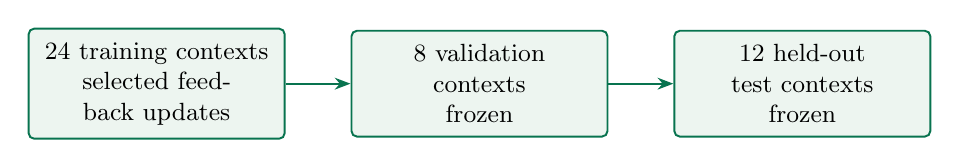
\begin{tikzpicture}[x=1cm,y=1cm]
\node[box,text width=2.9cm] (tr) at (0,0) {24 training contexts\\selected feedback updates};
\node[box,text width=2.9cm] (va) at (4.1,0) {8 validation contexts\\frozen};
\node[box,text width=2.9cm] (te) at (8.2,0) {12 held-out test contexts\\frozen};
\draw[arrow] (tr)--(va);\draw[arrow] (va)--(te);
\end{tikzpicture}\par
\end{center}
\uncover<2->{\Question{The learner predicts improvement, but the trial violates current. Accept?}
\Answer{Reject the trial. Keep a valid incumbent or escalate; reward does not grant permission.}}

\Source{\href{https://arxiv.org/abs/1003.0146}{Li et al.: LinUCB}; Recorded \texttt{LLM\_Response\_Selection.ipynb}; raw calls in \texttt{results/ensemble\_voltage\_pilot/}}
\Bridge{Does the frozen choice agree with the majority and pass a new check?}
\note{Read the reward in two branches. A passing trial can earn a bounded improvement reward relative to the incumbent cost, with a fixed trial charge. A rejected trial receives a negative reward. The 0.01 scaling and charge are design choices; the charge does not measure latency. Training consumes selected outcomes, although the audit records contain other outcomes for comparisons. Validation and test are frozen, avoiding feedback leakage. Five training orders reuse the same training contexts and are not five independent datasets. Ask learners how changing reward scaling might change selection without changing any electrical operating limit. This separates learning preferences from the hard verification contract.}
\end{frame}

\begin{frame}[t]{L4: verify the frozen choice with a new numerical trial}
\label{f:V22}
\small

\Checkpoint{L4}{Three minutes: run the full cell and explain the output.}
\begin{columns}[T]
\column{.59\textwidth}
\lstinputlisting[style=python,firstline=1,lastline=8]{snippets/L4.py}
\column{.38\textwidth}
\VoltageIdea{Before the trial}{Which canonical operation did the learner choose? Does it match the majority?}
\medskip
\uncover<2->{\VoltageIdea{After the trial}{Did the fresh gate pass? What current-step cost was obtained?}}
\medskip
\uncover<3->{\textbf{Default:} learner and vote select Q reduction; original-context $J\approx0.031082$.}
\end{columns}
\medskip
{\small This evaluates archived original choices in their original context. Do not subtract this cost from a changed L2 scenario's cost.}

\Source{Executed \texttt{Classroom\_Labs.ipynb}; \texttt{src/classroom\_labs.py}; Recorded \texttt{LLM\_Response\_Selection.ipynb}; raw calls in \texttt{results/ensemble\_voltage\_pilot/}}
\Bridge{Does learned selection beat a simpler supervisor across held-out cases?}
\note{Read the exact L4 code, then give participants three minutes. The stored selector chooses an operation using its frozen parameters. The numerical helper evaluates the selected trial again under the archived original context. The displayed predicted reward is a learned estimate, while the returned trial table contains newly calculated outcomes. Participants should check whether the canonical candidate matches the majority choice and whether it passes the engineering gate. In this recorded test, the learner and majority agree on reactive reduction. Do not subtract this cost from a modified L2 cost, because those are different contexts. Ask which outcome controls the recommendation if a predicted improvement conflicts with failed verification.}
\end{frame}

\begin{frame}[t]{A fair experiment can find no learned advantage}
\label{f:V23}
\small

{\small Recorded held-out MV pilot: 12 scenarios; lower $J$ is better under the same reduced-model contract.}
\medskip
\begin{center}
\begin{tabular}{lrr}
\hline
Selection method & Mean $J$ & Same-action full AC PASS\\\hline
Fixed numerical refinement & 0.03400656 & 0/12\\
Majority vote & 0.03398479 & 0/12\\
Frozen learned selector & 0.03398479 & 0/12\\\hline
\end{tabular}
\end{center}
\uncover<2->{\begin{columns}[T]
\column{.48\textwidth}\VoltageIdea{Observed}{Vote and learner tie on every held-out case.}
\column{.48\textwidth}\VoltageIdea{Diagnostic}{A posthoc fixed Q-reduction rule reproduces their choices without LLM calls.}
\end{columns}}
\uncover<3->{\VoltageIdea{What this supports}{Reproducible trials and explicit checking are demonstrated. Superior control from extra LLMs or a learned selector is not established.}}

\Source{Recorded \texttt{LLM\_Response\_Selection.ipynb}; raw calls in \texttt{results/ensemble\_voltage\_pilot/}}
\Bridge{How much additional decision time did the response pool require?}
\note{Present this result without framing a tiny cost change as general superiority. The majority vote and frozen learner tie on all twelve held-out MV cases. A simple posthoc rule that always selects the reactive reduction reproduces those choices without language-model calls. Because that rule was identified after inspecting results, label it a diagnostic rather than a predeclared baseline. The experiment demonstrates that bounded proposals, fresh verification and reproducible traces can be implemented. It does not demonstrate that additional LLMs or a learned selector are necessary for better control. Ask what new test set or task distribution would make the learner's contribution more convincing than the simpler supervisor.}
\end{frame}

\begin{frame}[t]{Report the latency of the entire decision path}
\label{f:V24}
\small

\begin{center}
\par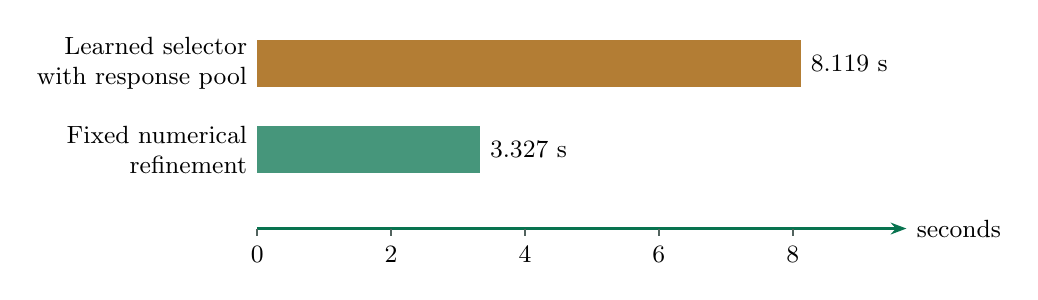
\begin{tikzpicture}[x=.85cm,y=1cm]
\draw[arrow] (0,0)--(9.7,0) node[right,font=\small]{seconds};
\foreach \x in {0,2,4,6,8}{\draw[slate] (\x,0)--(\x,-.1);\node[below,font=\small] at (\x,-.1){\x};}
\node[left,font=\small,align=right] at (0,1) {Fixed numerical\\refinement};
\fill[teal!75] (0,.7) rectangle (3.327,1.3);
\node[right,font=\small] at (3.327,1){3.327 s};
\uncover<2->{\node[left,font=\small,align=right] at (0,2.1) {Learned selector\\with response pool};
\fill[amber!85] (0,1.8) rectangle (8.119,2.4);
\node[right,font=\small] at (8.119,2.1){8.119 s};}
\end{tikzpicture}\par
\end{center}
{\small Recorded component times, reconstructed serial accounting for the held-out MV pilot. These are not guarantees for a deployed control room.}
\medskip
\begin{columns}[T]
\column{.48\textwidth}\VoltageIdea{Count all work}{Every pool selector pays for all three LLM responses, plus numerical trials and checks.}
\column{.48\textwidth}\VoltageIdea{Separate timing boundaries}{Training, model loading, token generation, actor inference and end-to-end execution are different quantities.}
\end{columns}

\Source{Recorded \texttt{LLM\_Response\_Selection.ipynb}; raw calls in \texttt{results/ensemble\_voltage\_pilot/}; \href{https://docs.ollama.com/api/chat}{Ollama chat API timing fields}}
\Bridge{What happens when the same chosen action is tested by a broader model?}
\note{The two reported times are reconstructed serial accounting from actual recorded components in the held-out pilot. They are not a guaranteed deployment response time and should not be confused with a new classroom timing measurement. Pool-based selectors share the cost of generating the three responses. The learned selector's small scoring operation is only one component of that total. Cold model loading, prompt processing, token generation and numerical checking can have very different scaling. Ask learners to draw the boundary around the quantity they want to compare. The engineering question is whether any incremental benefit justifies the additional decision latency under the intended operator workflow.}
\end{frame}

\begin{frame}[t]{L5 separates same-action auditing from AC replanning}
\label{f:V25}
\small

\Checkpoint{L5}{Default: fresh MV audit. Optional: full AC audit and a separate AC MPC solve.}
\begin{columns}[T]
\column{.54\textwidth}
\lstinputlisting[style=python,firstline=1,lastline=6]{snippets/L5.py}
{\small Enable \texttt{RUN\_OPENDSS} in L0 for the optional path. Run OpenDSS evaluations sequentially.}
\column{.43\textwidth}
\par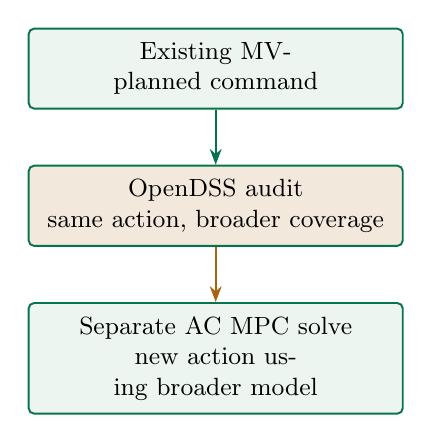
\begin{tikzpicture}[node distance=7mm]
\node[box,text width=4.4cm] (u) {Existing MV-planned command};
\node[box,fill=amber!15,text width=4.4cm,below=of u] (a) {OpenDSS audit\\same action, broader coverage};
\draw[arrow] (u)--(a);
\uncover<2->{\node[box,text width=4.4cm,below=of a] (m) {Separate AC MPC solve\\new action using broader model};
\draw[arrow,draw=amber] (a)--(m);}
\end{tikzpicture}\par
\end{columns}
\uncover<3->{\VoltageIdea{Two questions}{Does the old recommendation survive the audit? What would a planner using the broader model recommend instead?}}

\Source{Executed \texttt{Classroom\_Labs.ipynb}; \texttt{src/classroom\_labs.py}; \href{https://opendss.epri.com/}{EPRI OpenDSS documentation}}
\Bridge{Which model actually checks the requested operating scope?}
\note{Read the helper call before enabling its optional path. The same-action audit asks whether an existing recommendation survives a broader physical model. The separate AC MPC solve asks what command a planner using that broader model would propose. Mixing those questions can make model coverage look like an LLM improvement. The default classroom execution performs the MV check; enabling RUN\_OPENDSS in L0 requests the fresh AC audit and separate AC replanning in L5. The saved learner remains frozen. OpenDSS computations should be performed sequentially because the local engine has shared mutable state. Compare the status, limiting quantities and model scope rather than treating cross-model costs as an exact solver ranking.}
\end{frame}

\begin{frame}[t]{A reduced-model PASS can fail the full-feeder audit}
\label{f:V26}
\small

\begin{center}
\par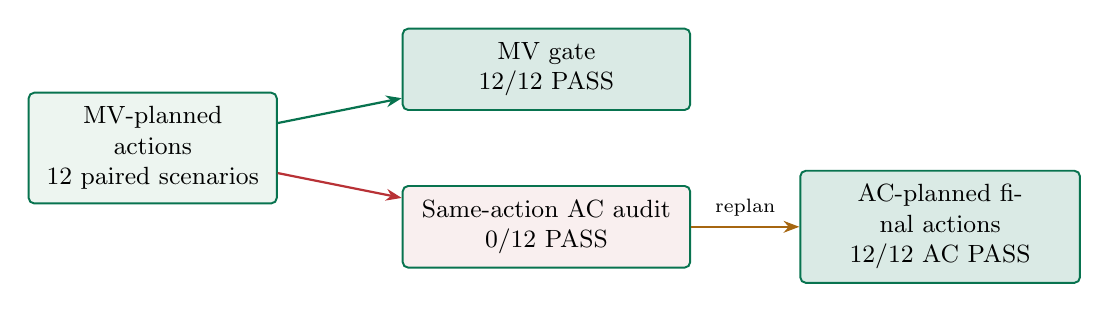
\begin{tikzpicture}[x=1cm,y=1cm]
\node[box,text width=2.8cm] (u) at (0,0) {MV-planned actions\\12 paired scenarios};
\node[box,fill=teal!15,text width=3.3cm] (mv) at (5,1) {MV gate\\12/12 PASS};
\node[box,fill=red!8,text width=3.3cm] (ac) at (5,-1) {Same-action AC audit\\0/12 PASS};
\draw[arrow] (u)--(mv);
\draw[arrow,draw=red] (u)--(ac);
\uncover<2->{\node[box,fill=teal!15,text width=3.2cm] (new) at (10,-1) {AC-planned final actions\\12/12 AC PASS};
\draw[arrow,draw=amber] (ac)--node[above,font=\scriptsize]{replan}(new);}
\end{tikzpicture}\par
\end{center}
\begin{columns}[T]
\column{.48\textwidth}\VoltageIdea{What changed}{Numerical equations and network/constraint coverage. The selector remained frozen.}
\column{.48\textwidth}\VoltageIdea{What did not follow}{This does not prove an LLM caused the better physical result, nor does PASS constitute human approval.}
\end{columns}
{\small Separately recorded 12-case pilot; not the output of one classroom L5 execution.}

\Source{Recorded \texttt{LLM\_Response\_Selection.ipynb}; raw calls in \texttt{results/ensemble\_voltage\_pilot/}}
\Bridge{With the broader model held fixed, does learned selection improve cost?}
\note{The table summarizes the separately recorded twelve paired scenarios, not the output of one L5 cell. The reduced model accepts all twelve final actions under its own scope, yet their same-action full-feeder audits fail. Planning with the AC backend returns actions that pass the full-feeder snapshot contract in these scenarios. The result is caused by the broader model and constraint coverage, with the selector still frozen. It cannot be attributed to more convincing Llama explanations. Within the AC pilot, the learned selector also does not establish superiority over fixed or uniform selection. Ask learners how a responsible operator packet should describe an MV-only recommendation when full MV/LV coverage was requested.}
\end{frame}

\begin{frame}[t]{The AC comparison still needs a strong numerical baseline}
\label{f:V27}
\small

\begin{columns}[T]
\column{.52\textwidth}
{\small Recorded paired AC pilot, 12 scenarios.}
\medskip
\begin{tabular}{lr}
\hline
Method & Mean current-step $J$\\\hline
MPC first action & 0.47172417\\
Fixed refinement & 0.47112138\\
Uniform pool selection & 0.47110513\\
Majority vote & 0.47138488\\
Frozen learned selection & 0.47138488\\\hline
\end{tabular}
\column{.45\textwidth}
\VoltageIdea{Interpretation}{Vote and learner tie. The learned selector does not beat the fixed or uniform comparators here.}
\medskip
\uncover<2->{\VoltageIdea{Check the raw policy too}{Only 1/12 raw SAC actions passes the AC gate in this pilot. A fast proposal is not automatically usable.}}
\end{columns}
\uncover<3->{\VoltageIdea{Why this is a scientific result}{Hold scenario, feasible set, budget and evaluation boundary constant. Attribute changes to the controller, model, information or orchestration mechanism that actually changed.}}
{\small Do not compare AC and MV objective means as a pure solver ranking: the modeled voltage sets differ.}

\Source{Recorded \texttt{LLM\_Response\_Selection.ipynb}; raw calls in \texttt{results/ensemble\_voltage\_pilot/}}
\Bridge{What should the operator receive after this whole workflow?}
\note{The broader AC model improves the relevance of the checked constraint set, but that does not establish a benefit from the learned response selector. In the twelve paired AC scenarios, the frozen learner and majority vote tie, and their mean current-step cost is worse than the fixed-refinement and uniform-pool comparators. The raw SAC proposal passes only one of twelve AC checks in this pilot, illustrating transfer limitations. Explain that every listed final recommendation still needs its declared physical gate. Do not compare the AC mean directly with the MV mean as if they measured an identical voltage set. A rigorous architecture study isolates the contribution of each changed component and reports negative results alongside successes.}
\end{frame}

\begin{frame}[t]{The operator receives a scoped recommendation and its evidence}
\label{f:V28}
\small

\begin{columns}[T]
\column{.62\textwidth}
\begin{tabular}{p{2.0cm}p{6.0cm}}
\hline
Stage & Returned evidence in this lesson\\\hline
Awareness & Load, rating fraction, requested scope, revision\\[1mm]
Planning & MPC and SAC candidate commands\\[1mm]
Simulation & New voltages, currents and objective\\[1mm]
Verification & PASS / failures; candidate-bound model evidence\\[1mm]
LLM optimizer & Permitted trial and recorded public rationale\\\hline
\end{tabular}
\column{.35\textwidth}
\par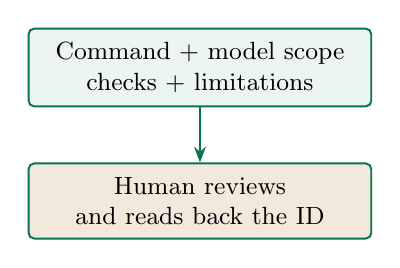
\begin{tikzpicture}[node distance=7mm]
\node[box,text width=4cm] (pk) {Command + model scope\\checks + limitations};
\node[box,fill=amber!15,text width=4cm,below=of pk] (h) {Human reviews\\and reads back the ID};
\draw[arrow] (pk)--(h);
\end{tikzpicture}\par
\uncover<2->{\medskip\VoltageIdea{Full scope requested?}{An MV-only PASS remains HOLD for a request requiring full MV/LV coverage.}}
\end{columns}
\uncover<3->{\VoltageIdea{Demonstrated benefit and boundary}{The workflow makes assumptions, trials and failures inspectable. Extra LLMs did not demonstrate better control here. Readback is advisory, not equipment dispatch.}}

\Source{Executed \texttt{Classroom\_Labs.ipynb}; \texttt{src/classroom\_labs.py}, L1--L5 and L12; Recorded \texttt{LLM\_Response\_Selection.ipynb}; raw calls in \texttt{results/ensemble\_voltage\_pilot/}}
\Bridge{After the break: what changes when the action is a topology rather than a setpoint?}
\note{Close the voltage chapter with the complete path and the actual findings. The numerical controllers supplied proposed settings. The language models supplied bounded refinement choices and public explanations. Voting and frozen learned selection tied in the held-out MV pilot. Broader-model checking revealed that the reduced-model recommendations did not meet the requested full-feeder scope. These are valuable workflow lessons without a claim of universal agentic control superiority. The operator must see the command, scenario, evidence, failed checks, remaining assumptions and required scope. Readback remains advisory and does not dispatch equipment. Invite one participant to name a demonstrated benefit and another to name a limitation, then take the scheduled ten-minute break before restoration.}
\end{frame}




\begin{frame}[t]{Ten-minute break: 80--90 minutes}
\label{f:BREAK}
\vspace{.7cm}
\begin{center}\Large Keep your voltage result and its model scope.\end{center}
\vspace{.5cm}
\Idea{What changes after the break?}{For voltage support, we adjusted inverter controls on a given network. After a fault, some paths are unavailable. We must choose which loads the remaining paths can serve.}
\Question{Would the largest number of restored kilowatts always be the right objective?}
\Source{Workshop timetable. Take the full ten-minute break.}
\Bridge{Which loads should the remaining network support?}
\note{Take the full break. Participants do not need to install packages or run a new cell during it. Before leaving the voltage chapter, ask them to keep a note of the action, which model checked it, and which limits were evaluated. At the restart, recall that inverter settings are continuous decisions. Restoration introduces discrete load pickup and network choices. That contrast creates a reason for a different planning method instead of assigning MPC to every problem. The next case will make the priorities visible using six numbered nodes, a failed connection and two optional ties.}
\end{frame}
\section{Restoration: paths, capacity and priorities}
% Native, editable teaching diagrams. R01--R18; no appendix material.
\newcommand{\RestMap}[1]{%
  \node[circle,draw=teal,fill=pale,minimum size=7mm,font=\small] (r0) at (0,1) {0};
  \node[circle,draw=teal,fill=pale,minimum size=7mm,font=\small] (r1) at (1.7,2.2) {1};
  \node[circle,draw=amber,fill=amber!12,minimum size=7mm,font=\small] (r2) at (3.7,2.2) {2};
  \node[circle,draw=teal,fill=pale,minimum size=7mm,font=\small] (r3) at (5.5,1) {3};
  \node[circle,draw=teal,fill=pale,minimum size=7mm,font=\small] (r4) at (3.7,-.2) {4};
  \node[circle,draw=amber,fill=amber!12,minimum size=7mm,font=\small] (r5) at (1.7,-.2) {5};
  \draw[slate] (r0)--(r1);
  \draw[red,dashed,very thick] (r1)--node[midway,fill=white,text=red,font=\large] {$\times$}(r2);
  \draw[slate] (r2)--(r3)--(r4);
  \draw[slate] (r2)--(r5);
  \draw[amber,dashed,thick] (r1)--node[left,font=\scriptsize,fill=white]{100 kW}(r5);
  \draw[amber,dashed,thick] (r0) to[out=-75,in=205] (r4);
  \node[font=\scriptsize,text=amber,align=center] at (0,-.55) {tie 0--4\\#1 kW};
  \node[font=\scriptsize,above=1mm of r1] {40 kW};
  \node[font=\scriptsize,above=1mm of r2,text=amber] {60 kW, critical};
  \node[font=\scriptsize,right=1mm of r3] {70 kW};
  \node[font=\scriptsize,below=1mm of r4] {50 kW};
  \node[font=\scriptsize,below=1mm of r5,text=amber] {30 kW, critical};
  \node[font=\scriptsize,left=1mm of r0] {source};
}

\begin{frame}[t]{A fault changes the paths that are available}
\label{f:R01}
\begin{columns}[T,onlytextwidth]
\column{.59\textwidth}
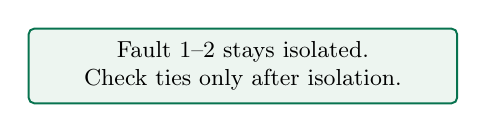
\begin{tikzpicture}[scale=.93,transform shape]
\RestMap{40}
\uncover<2->{\node[box,text width=5.5cm] at (2.6,-1.55) {Fault 1--2 stays isolated.\\Check ties only after isolation.};}
\end{tikzpicture}
\column{.39\textwidth}
\Idea{A small, transparent fixture}{Six nodes; five loads; one failed segment; two optional ties. Amber nodes have higher service priority.}
\Question{Can we simply reconnect the failed segment?}
\Answer{No. Its availability is fixed to zero. Planning must find another admissible path.}
\end{columns}
\Source{Fresh classroom fixture: Classroom\_Labs L6; src/standard\_formulations.py. Restoration context: \href{https://doi.org/10.1109/TPWRS.2017.2720122}{Chen et al., IEEE TPWRS, 2018}.}
\Bridge{What can each alternative path carry?}
\note{Begin with the physical picture, not an optimization acronym. Node zero is the available source. The interrupted segment connects nodes one and two, and is unavailable throughout the experiment. The dashed amber links are candidate ties, not commands already issued. Nodes two and five are designated critical in this classroom fixture. Explain that the drawing is a six-node active-power transport example, not a reduced drawing of the full Greensboro feeder. Its purpose is to expose the decisions clearly enough to check them by hand. Ask the audience to point to the failed segment and identify a route that avoids it. Reveal the isolation statement before discussing any restoration action. A real switching procedure additionally needs protection, equipment status, work permits and operator authority, which this static fixture does not establish.}
\end{frame}

\begin{frame}[t]{Two ties create choices, with different bottlenecks}
\label{f:R02}
\begin{columns}[T,onlytextwidth]
\column{.60\textwidth}
\begin{tikzpicture}[scale=.93,transform shape]
\RestMap{40}
\uncover<2->{\draw[teal,line width=2pt,->] (r0)--(r1);\draw[teal,line width=2pt,->] (r1)--(r5);\draw[teal,line width=2pt,->] (r5)--(r2);}
\uncover<3->{\draw[blue,line width=2pt,->] (r0) to[out=-75,in=205] (r4);}
\end{tikzpicture}
\column{.38\textwidth}
\Idea{Follow the power}{The route $0\!\to\!1\!\to\!5\!\to\!2$ uses the 100 kW tie. The other tie has only 40 kW in this first case.}
\Question{Can the 40 kW tie pick up the entire 50 kW load at node 4?}
\uncover<3->{\textcolor{red}{No: $50>40$.} Loads are indivisible here; partial pickup is excluded.}
\end{columns}
\Source{Fixture and binary pickup assumption: Classroom\_Labs L6; standard\_formulations.restoration\_graph. Blue and teal paths are explanatory alternatives, not a switching sequence.}
\Bridge{Does an energized node have to serve its local load?}
\note{Trace the teal route with a pointer while it appears. The hundred-kilowatt tie between nodes one and five must carry the downstream demand that the chosen tree places behind it. Node one's own forty-kilowatt demand can be supplied before that bottleneck. The other tie supplies the lower side of the diagram, but at forty kilowatts it cannot pick up the fifty-kilowatt block at node four. That conclusion relies on the all-or-nothing pickup assumption. It would change if loads could be divided into smaller controllable groups. The colors describe routes for reasoning; the slide does not certify a safe temporal switching sequence. Ask participants to distinguish a branch rating from the total rating of the source. The next distinction is between energizing a bus so power can pass through it and reconnecting that bus's local demand.}
\end{frame}

\begin{frame}[t]{A node can carry power while its load stays disconnected}
\label{f:R03}
\begin{columns}[T,onlytextwidth]
\column{.60\textwidth}
\begin{tikzpicture}[scale=.93,transform shape]
\RestMap{40}
\draw[teal,line width=1.7pt] (r0)--(r1)--(r5)--(r2)--(r3);
\node[box,text width=5.7cm] at (2.7,-1.55) {Example: serve nodes 1, 3, 5; pass through node 2.};
\uncover<2->{\node[draw=red,fill=white,rounded corners,font=\scriptsize,align=center] at (4.5,3.35) {node 2 energized\\local 60 kW disconnected};}
\end{tikzpicture}
\column{.38\textwidth}
\Idea{Two different binary decisions}{$y_i=1$: node $i$ is energized.\par $s_i=1$: its load is picked up.\par\smallskip We require $s_i\le y_i$.}
\Question{Why is equality $s_i=y_i$ too restrictive?}
\Answer{It would forbid a useful transit node whose own load remains shed.}
\end{columns}
\Source{Original schematic of a feasible six-node plan; binary pickup/energization model in src/standard\_formulations.py.}
\Bridge{How do we compare feasible pickup decisions?}
\note{This is an important modeling distinction that is easy to miss when a diagram uses one color for everything. The illustrated path can carry power through node two while leaving its sixty-kilowatt demand disconnected. In the example, the tie between one and five carries thirty kilowatts for node five plus seventy for node three, exactly one hundred kilowatts. Node one's forty kilowatts are supplied upstream. The total picked up is therefore one hundred forty kilowatts. Define the energized variable and the pickup variable in words before showing their inequality. The figure is an explicit feasible explanation of the unweighted service level, not a claim that every optimizer returns this exact edge list. Different optimal trees can exist. Invite participants to explain why a transit node still needs valid energized connectivity even when its local pickup variable is zero.}
\end{frame}

\begin{frame}[t]{A capacity budget turns priorities into a real choice}
\label{f:R04}
\begin{columns}[T,onlytextwidth]
\column{.54\textwidth}
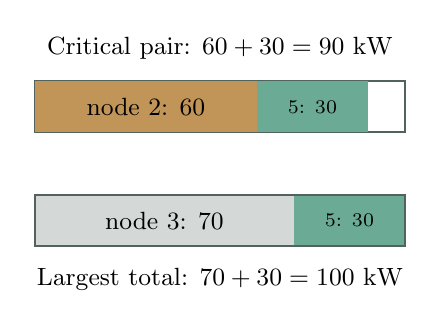
\begin{tikzpicture}[x=.047cm,y=1cm]
\draw[slate] (0,0) rectangle (100,.65);
\fill[amber!70] (0,0) rectangle (60,.65);
\fill[teal!60] (60,0) rectangle (90,.65);
\node[font=\small] at (30,.32) {node 2: 60};
\node[font=\scriptsize] at (75,.32) {5: 30};
\node[font=\small,above] at (50,.8) {Critical pair: $60+30=90$ kW};
\uncover<2->{\fill[slate!25] (0,-1.45) rectangle (70,-.8);\fill[teal!60] (70,-1.45) rectangle (100,-.8);\draw[slate] (0,-1.45) rectangle (100,-.8);\node[font=\small] at (35,-1.12) {node 3: 70};\node[font=\scriptsize] at (85,-1.12) {5: 30};\node[font=\small,below] at (50,-1.6) {Largest total: $70+30=100$ kW};}
\end{tikzpicture}
\column{.43\textwidth}
\Idea{The 100 kW tie is the budget}{Both choices also serve node 1's 40 kW upstream.\par Critical pair: total 130; critical 90.\par Largest total: total 140; critical 30.}
\Question{Which outcome should a critical-service policy prefer?}
\Answer{The answer depends on the stated objective, not on how persuasive its explanation sounds.}
\end{columns}
\Source{Hand-checkable choices at tie 0--4 capacity 40 kW; exact optima confirmed by Classroom\_Labs L6. Bars represent kW, not physical line lengths.}
\Bridge{How do we put that service policy into mathematics?}
\note{Use the bars as a budget, with each indivisible load consuming part of the hundred-kilowatt tie capacity. The top choice carries the two critical loads, sixty plus thirty kilowatts, leaving ten unused. That unused capacity cannot serve any remaining complete load block. The bottom choice uses all one hundred kilowatts to carry seventy plus thirty. Both plans also serve forty kilowatts at node one upstream, so their total service is one hundred thirty and one hundred forty respectively. Ask for a preference before revealing the policy interpretation. The lower total service is not evidence that the weighted optimizer failed. It can be the intended consequence of protecting critical demand. Equally, the higher total service is not a mistake under an explicitly unweighted objective. This prepares a fair comparison: same feasible network, transparent objectives, and both total and critical service reported.}
\end{frame}

\begin{frame}[t]{Compare outcomes before comparing algorithms}
\label{f:R05}
\begin{center}
\begin{tabular}{lrrr}
\toprule
Same 40 kW tie case & Total served & Critical served & Critical share served\\
\midrule
Maximize total kW & 140 kW & 30 kW & $30/90$\\
\uncover<2->{Maximize weighted kW & 130 kW & 90 kW & $90/90$}\\
\bottomrule
\end{tabular}
\end{center}
\Idea{What the experiment establishes}{Changing the service objective changes who benefits. It does not establish an advantage caused by an LLM or by the word ``agentic.''}
\Question{What must stay matched to isolate an agentic workflow effect?}
\Answer{The objective, candidate tools, physical limits, information and verification rules.}
\Source{Fresh six-node experiment: Classroom\_Labs L6, weighted MILP versus unweighted exact enumeration; both use the same feasible constraints.}
\Bridge{What does a priority weight of ten actually mean?}
\note{Keep the table visible long enough for participants to read both columns. Reporting only total service would conceal the reason the weighted formulation was chosen. Reporting only critical service would conceal the sacrifice in ordinary service. The first comparison intentionally changes the objective, so it is a policy comparison. It is not a controlled test of language-model orchestration. The unweighted baseline is solved exactly by enumeration on the same small network and constraints; it is not a deliberately weak random baseline. The weighted MILP is also checked against exhaustive enumeration. Later we will compare a fixed supervisor and an LLM supervisor with matched objectives and tools, using a separate archived feeder experiment. Ask the audience to list what must be held equal in that later comparison. This distinction helps them avoid attributing every favorable result to the framework.}
\end{frame}

\begin{frame}[t]{The objective is an explicit, inspectable service policy}
\label{f:R06}
\[
\max \sum_{i=1}^{5} w_i d_i s_i,
\qquad w_2=w_5=10,\qquad w_1=w_3=w_4=1.
\]
\begin{columns}[T,onlytextwidth]
\column{.48\textwidth}
\Idea{Critical-pair choice}{$10(60+30)+40=\mathbf{940}$\par weighted kW; 130 actual kW.}
\column{.48\textwidth}
\uncover<2->{\Idea{Maximum-total choice}{$10(30)+70+40=\mathbf{410}$\par weighted kW; 140 actual kW.}}
\end{columns}
\small $d_i$: load demand in kW; $w_i$: dimensionless priority; $s_i\in\{0,1\}$: pickup.
\Question{Does weight ten guarantee critical-first service on every possible network?}
\Answer{No. Strict priority requires a lexicographic objective or a proven sufficiently large weight.}
\Source{Classroom priority policy: standard\_formulations.restoration\_graph. Weighted restoration objectives: \href{https://doi.org/10.1109/TPWRS.2017.2720122}{Chen et al., 2018}.}
\Bridge{Which constraints make a high-scoring plan physically admissible?}
\note{Read the expression aloud as demand multiplied by a priority and a pickup decision, then summed over loads. Distinguish actual kilowatts from the weighted score. The critical-pair plan earns nine hundred forty weighted kilowatts, while the illustrated maximum-total plan earns four hundred ten. The factor ten is an instructional policy choice, not an empirical estimate of a hospital's value or an industry-wide standard. A finite weight can be outweighed by sufficiently much ordinary demand, so it does not automatically encode strict critical-first restoration. If strict priority is required, solve critical service first and preserve that optimum in a second objective, or justify a bound on the weight. The planner should expose this assumption to the operator rather than letting an LLM silently invent priorities. Now move from scoring plans to checking which plans are feasible.}
\end{frame}

\begin{frame}[t]{Planning: binary pickup and topology decisions}
\label{f:R07}
\begin{columns}[T,onlytextwidth]
\column{.48\textwidth}
\begin{tabular}{ll}
\toprule Symbol & Meaning\\\midrule
$s_i\in\{0,1\}$ & load $i$ picked up\\
$y_i\in\{0,1\}$ & node $i$ energized\\
$z_e\in\{0,1\}$ & edge $e$ closed\\
$P_e\in\mathbb R$ & signed active flow, kW\\
$\bar P_e$ & edge capacity, kW\\\bottomrule
\end{tabular}
\column{.48\textwidth}
\begin{align*}
s_i&\le y_i, & y_0&=1,\\
z_{ij}&\le y_i, &z_{ij}&\le y_j,\\
z_{1,2}&=0.&&
\end{align*}
\uncover<2->{\Idea{Interpret each line}{Picked-up loads need energized nodes; closed edges need energized endpoints; the fault stays isolated.}}
\end{columns}
\Question{Which of these rules prevents a disconnected energized island?}
\Answer{None yet. Connectivity must be imposed separately.}
\Source{Fresh MILP implementation: src/standard\_formulations.py. Radiality and connectivity: \href{https://arxiv.org/abs/1912.05185}{Wang et al., 2020}.}
\Bridge{How do flow balance and capacity restrict pickup?}
\note{Introduce one decision type at a time and connect it to the preceding diagrams. The pickup variable describes demand, the energized variable describes the usable network, and the edge variable describes the selected topology. Signed flow needs an arbitrary reference orientation; a negative value simply means power travels the other way. The source is fixed energized, and the failed segment is fixed open. The endpoint constraints prevent a selected line from attaching to a node labeled de-energized. These are necessary logical conditions, but they do not prove that every energized node is reachable from the source. Pause on that omission. An isolated cycle could satisfy many local conditions while being impossible to supply. The next two slides add active-power transport and source connectivity. This modular construction explains what each constraint contributes rather than presenting one intimidating formulation without interpretation.}
\end{frame}

\begin{frame}[t]{Power balance says where every picked-up kilowatt comes from}
\label{f:R08}
\[
\underbrace{\sum_{e} A_{ie}P_e}_{\text{net active power entering node }i}
=\underbrace{d_i s_i}_{\text{picked-up demand}},\quad i\ne0,
\qquad -\bar P_e z_e\le P_e\le\bar P_e z_e.
\]
\begin{center}
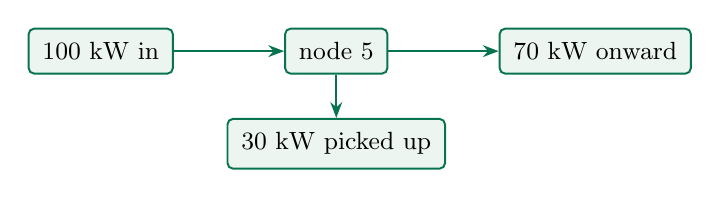
\begin{tikzpicture}[node distance=1.4cm]
\node[box] (in) {100 kW in};
\node[box,right=of in] (node) {node 5};
\node[box,right=of node] (out) {70 kW onward};
\node[box,below=.55cm of node] (load) {30 kW picked up};
\draw[arrow] (in)--(node);\draw[arrow] (node)--(out);\draw[arrow] (node)--(load);
\end{tikzpicture}
\end{center}
\small $A_{ie}=+1$ for an edge entering $i$, $-1$ leaving it, zero otherwise.
\uncover<2->{\Idea{Know the model boundary}{This is lossless active-power transport. Voltage, reactive power, AC losses and protection are not certified.}}
\Source{Classroom\_Labs L6; active-transport formulation in src/standard\_formulations.py. This six-node model is separate from the archived feeder power-flow checks.}
\Bridge{How can we prove every energized node has a source path?}
\note{Use the small flow diagram to show that balance is bookkeeping with a physical interpretation. One hundred kilowatts arrive at node five, thirty are consumed locally, and seventy continue downstream. With the stated incidence convention, incoming flows enter positively and outgoing flows negatively. At an open edge, the binary variable is zero, forcing its flow to zero. At a closed edge, the same inequalities bound the magnitude by the rating. The source balance is handled as the supply needed to satisfy non-source demand. State the model limitation clearly: a feasible active-transport solution is not an AC security certificate. It ignores voltage, reactive power, losses and protection behavior. That simplicity is deliberate for a hand-checkable lesson. The later archived feeder result uses additional power-flow evidence, but must not be confused with this exact MILP fixture.}
\end{frame}

\begin{frame}[t]{Edge counts alone do not prove a source-connected tree}
\label{f:R09}
\begin{columns}[T,onlytextwidth]
\column{.43\textwidth}
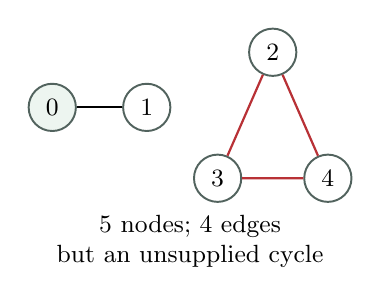
\begin{tikzpicture}[every node/.style={circle,draw=slate,minimum size=6mm,font=\small}]
\node[fill=pale] (a) at (0,1) {0};\node (b) at (1.2,1) {1};
\node (c) at (2.8,1.7) {2};\node (d) at (2.1,.1) {3};\node (e) at (3.5,.1) {4};
\draw (a)--(b);\draw[red,thick] (c)--(d)--(e)--(c);
\node[draw=none,rectangle,align=center,font=\small] at (1.75,-.7) {5 nodes; 4 edges\\but an unsupplied cycle};
\end{tikzpicture}
\column{.55\textwidth}
\uncover<2->{\begin{align*}
\sum_e A_{ie}f_e&=y_i &&(i\ne0),\\
-5z_e\le f_e&\le5z_e,\\
\sum_e z_e&=\sum_i y_i-1.
\end{align*}}
\small $f_e$: fictitious connectivity flow, not electrical kW. Every energized non-source node consumes one unit. Five is the maximum number of such nodes.
\end{columns}
\Idea{Two jobs, two conditions}{Commodity flow proves reachability. Reachability plus the edge count gives a tree on the energized nodes.}
\Source{Original counterexample; single-commodity connectivity and radiality: \href{https://arxiv.org/abs/1912.05185}{Wang et al., 2020}; classroom MILP.}
\Bridge{How do we check a small MILP without trusting its solver blindly?}
\note{The left-hand counterexample is a separate five-node sketch, not the six-node restoration fixture. It has the familiar tree edge count but is disconnected: the source supplies one short component while three other nodes form a cycle. This makes the missing condition visible. Reveal the fictitious flow equations and explain that these units are proof tokens. Every energized non-source node must receive one token through selected edges, so an island without the source cannot satisfy the summed balances. The source provides the required tokens. The bound of five is enough because the classroom network has five non-source nodes. Once all selected energized nodes are connected, exactly one fewer edge than nodes eliminates cycles. Emphasize that this proves a static graph property. It does not address the time ordering of switching, transient stability or protection coordination.}
\end{frame}

\begin{frame}[t]{Verification uses an independent, exhaustive small-case check}
\label{f:R10}
\begin{center}
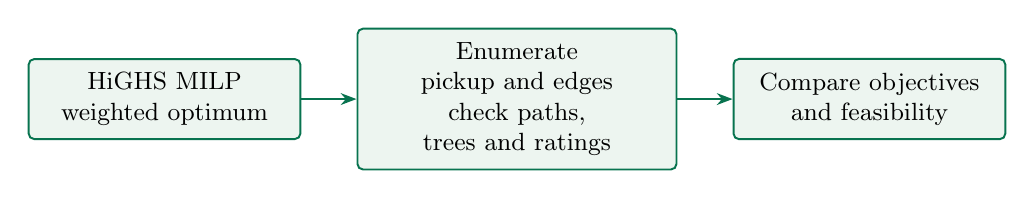
\begin{tikzpicture}[node distance=.7cm]
\node[box,text width=3.1cm] (m) {HiGHS MILP\\weighted optimum};
\node[box,text width=3.7cm,right=of m] (e) {Enumerate pickup and edges\\check paths, trees and ratings};
\node[box,text width=3.1cm,right=of e] (v) {Compare objectives\\and feasibility};
\draw[arrow] (m)--(e);\draw[arrow] (e)--(v);
\end{tikzpicture}
\end{center}
\Idea{Two solves within the MILP method}{First maximize weighted service. Then preserve that optimum and minimize selected edge count, with a small edge-index tie-breaker.}
\Question{Does minimizing selected edges minimize switching operations?}
\Answer{No. Operation count needs the initial switch states and a sequence-aware model.}
\small Exhaustive enumeration is practical because this fixture has only six nodes. It is a verification aid, not a proposed large-feeder algorithm.
\Source{Classroom\_Labs L6; standard\_formulations.solve\_restoration\_milp and \_enumerate\_restoration.}
\Bridge{Can your run reproduce the service trade-off?}
\note{Explain what independent means here. The enumeration routine loops over candidate edge sets and pickup choices, checks source reachability, the tree property and branch loading, and computes the service objective. It does not simply ask the MILP solver whether its own answer is acceptable. Agreement provides a strong check for this finite small fixture, although it does not prove that the simplified physical model covers every operational hazard. The second optimization pass preserves the best weighted service and prefers fewer energized edges, with a small index-based tie-breaker. Avoid calling that minimum switching: without initial switch positions and a temporal sequence, those are different quantities. The exhaustive method scales poorly, which is why it belongs in a small educational verification exercise. Ask participants to predict the forty-kilowatt result before running the sweep, so the computation tests a reasoned expectation.}
\end{frame}

\begin{frame}[fragile,t]{Hands-on: vary the bottleneck, keep the policy visible}
\label{f:R11}
\Checkpoint{L6}{Eight minutes: run the full cell, then compare 40, 80 and 100 kW.}
\lstinputlisting[style=python,firstline=1,lastline=5]{snippets/L6.py}
\begin{columns}[T,onlytextwidth]
\column{.48\textwidth}
\Idea{Before running}{Predict total and critical pickup at 40 kW. Then predict whether every increase in capacity must increase service.}
\column{.48\textwidth}
\uncover<2->{\Idea{Read the result}{Confirm MILP/enumeration agreement. Record both service measures and the elapsed solve/check time. Explain one plateau.}}
\end{columns}
\small Run the entire L6 cell; the displayed excerpt only locates the experiment. Samples are discrete capacities, not a continuous response curve.
\Source{Exact excerpt: Classroom\_Labs.ipynb, L6 lines 1--5. Fresh results use the six-node active-transport fixture.}
\Bridge{What causes a flat region in the capacity experiment?}
\note{Give participants the full eight minutes rather than using the lab slide as another lecture slide. Ask them to run the entire L6 cell, which includes the plot and the assertion that the weighted MILP matches the independent exhaustive check. The visible five lines identify the parameters and the result table. Participants should record total pickup, critical pickup and the measured runtime from their own environment. The runtime in this cell includes the fresh sweep and independent checks; it is not a single MILP solve or LLM latency. If someone changes the capacity samples, have them keep a note of the change so comparisons remain interpretable. The key explanation is a plateau: binary loads come in blocks, so extra capacity may remain unusable until it is large enough to connect another whole load.}
\end{frame}

\begin{frame}[t]{More capacity can produce the same discrete pickup}
\label{f:R12}
\begin{center}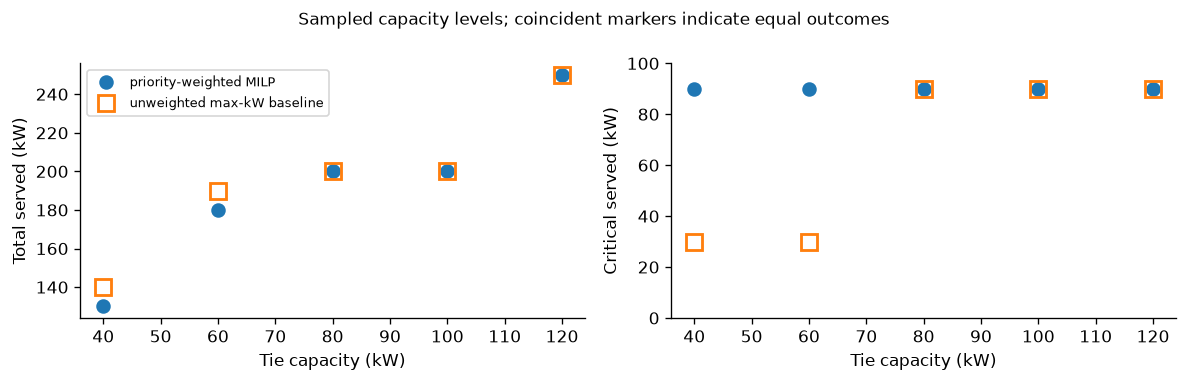
\includegraphics[width=.87\linewidth,height=3.4cm,keepaspectratio]{figures/classroom_restoration.png}\end{center}
\Idea{Two ratings, same pickup}{At 80 and 100 kW: weighted service is 200 kW total, including all 90 critical kW.}
\Question{Is the flat step evidence that capacity has no value?}
\Answer{No. It reflects indivisible load blocks and the available routes at these sampled ratings.}
\Source{Original computed figure: Classroom\_Labs L6 / classroom\_restoration.png. Same feasible constraints; weighted versus unweighted objectives.}
\Bridge{Where do the five agent stages add structure to this calculation?}
\note{Point first to the axes and the discrete sample markers. The plot compares policy choices at a set of tie capacities, not a continuously optimized physical design. At eighty and one hundred kilowatts, the weighted solution serves two hundred kilowatts in total and all ninety kilowatts of critical demand. A rating increase does not always admit another indivisible load block. The figure also lets participants see where objectives coincide, which is as important as the point where they differ. Do not interpret coincident markers as evidence that only one method ran. Both outcomes are plotted. Ask a participant to relate one marker back to a feasible path and the branch bottleneck from the earlier diagrams. Finish by distinguishing optimization quality from workflow quality: the next slide shows how the calculation becomes a traceable proposal, with assumptions and checks attached.}
\end{frame}

\begin{frame}[t]{The workflow surrounds the solver with evidence and decisions}
\label{f:R13}
\small
\renewcommand{\arraystretch}{1.12}
\begin{tabularx}{\linewidth}{>{\bfseries\raggedright\arraybackslash}p{2.35cm}>{\raggedright\arraybackslash}p{4.4cm}>{\raggedright\arraybackslash}X}
\toprule Stage & Specific method & Output that can be checked\\\midrule
Awareness & Topology and status checks & Fault 1--2; ratings; critical nodes 2, 5\\
Planning & Weighted restoration MILP & Pickup vector and selected edges\\
Simulation & Active-power transport & Per-edge demand and capacity margins\\
Verification & Independent enumeration & Feasible and objective agreement\\
LLM Optimizer & Allowed refinement request & Proposed next calculation, with rationale\\\bottomrule
\end{tabularx}
\uncover<2->{\Idea{Scope matters}{L6--L7 run fresh numerical and binding checks. L10 replays the full five-stage language trace from the separate archived feeder experiment.}}
\Source{Classroom\_Labs L6--L7, L10; proposal\_complete\_workflow.json. This table describes stage roles; L6 does not make five live LLM calls.}
\Bridge{What happens when the network rating changes after verification?}
\note{Read each row as a method producing a concrete output, rather than as five people having a conversation. Awareness binds the request to a topology and trusted ratings. Planning chooses pickups and edges. Simulation evaluates the transport consequences. Verification checks feasibility and, in this small case, agreement with an exhaustive optimum. The LLM optimizer may propose an allowed refinement or explain a tool result, but it does not override a failed capacity check. Be precise about what students are executing. L6 and L7 provide fresh numerical and evidence-binding experiments. L10 displays the full archived five-stage trace from a different feeder fixture. It would be misleading to imply that L6 itself makes all those language calls. The common framework is the contract among stages, while the physical models and numerical methods vary with the task.}
\end{frame}

\begin{frame}[fragile,t]{Hands-on: old evidence does not certify a changed rating}
\label{f:R14}
\Checkpoint{L7}{Four minutes: run the full cell, then explain the two Boolean results.}
\lstinputlisting[style=python,firstline=7,lastline=10]{snippets/L7.py}
\begin{center}
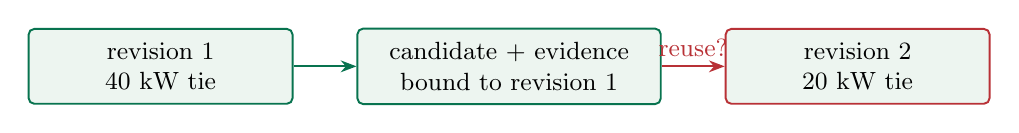
\begin{tikzpicture}[node distance=.8cm]
\node[box,text width=3cm] (a) {revision 1\\40 kW tie};
\node[box,text width=3.5cm,right=of a] (b) {candidate + evidence\\bound to revision 1};
\node[box,text width=3cm,right=of b,draw=red] (c) {revision 2\\20 kW tie};
\draw[arrow] (a)--(b);\draw[arrow,red] (b)--node[above,font=\small]{reuse?}(c);
\end{tikzpicture}
\end{center}
\Answer{Original binding: True. Changed request with old evidence: False. HOLD and re-solve.}
\Source{Exact excerpt: Classroom\_Labs L7 lines 7--10; lab.bind\_evidence and lab.bound\_to. Binding checks identity, not physical feasibility by itself.}
\Bridge{What additional evidence appears in the larger archived feeder case?}
\note{This exercise tests a workflow failure that can occur even when the original optimizer worked perfectly. The request changes from a forty-kilowatt tie rating at revision one to twenty kilowatts at revision two. The previous candidate and its evidence remain associated with the original request. The binding check should return true for that original request and false for the changed request. That failure means the old result is not valid evidence for the new contract; it does not independently prove that the old pickup is physically infeasible. A new constrained solve is required to decide that. Ask participants to name other changes that should invalidate evidence, such as topology, priorities, measurement provenance or the model version. The intended benefit is preventing stale recommendations from being presented as current checked actions, not improving the MILP objective.}
\end{frame}

\begin{frame}[t]{Archived feeder: an attractive pickup can fail a thermal check}
\label{f:R15}
\begin{columns}[T,onlytextwidth]
\column{.51\textwidth}
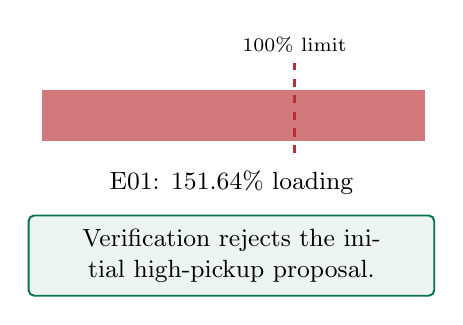
\begin{tikzpicture}[x=.032cm,y=1cm]
\fill[red!65] (0,0) rectangle (151.639,.65);
\draw[red,thick,dashed] (100,-.15)--(100,1);
\node[font=\scriptsize,above] at (100,1) {100\% limit};
\node[font=\small,below] at (75,-.25) {E01: 151.64\% loading};
\node[box,text width=4.8cm] at (75,-1.45) {Verification rejects the initial high-pickup proposal.};
\end{tikzpicture}
\column{.46\textwidth}
\Idea{Different fixture; explicit scope}{Archived MV feeder; synthetic short bypass; 100 A limit; ideal LV aggregation. No time-ordered switching certificate.}
\uncover<2->{\Idea{Refine, simulate, verify again}{A permitted shedding refinement produces a passing candidate: 1843.61 kW served, including 474.04 kW critical.}}
\end{columns}
\Source{ARCHIVED ACTUAL: proposal\_complete\_workflow.json, restoration / lindistflow3. Initial E01 loading 151.639\%; final verified SHED\_075.}
\Bridge{What did Llama actually say, and which statement required correction?}
\note{Make the fixture change explicit before presenting the numbers. We have left the six-node classroom graph and are inspecting an archived medium-voltage feeder workflow. It has a synthetic bypass catalog and an ideal low-voltage aggregation assumption. In the LinDistFlow3 run, the initial high-pickup candidate overloads the bypass to about one hundred fifty-two percent of its rating. That numerical result triggers rejection regardless of its language explanation. A permitted refinement sheds a specified fraction of ordered noncritical load objects, after which a candidate passes the modeled constraints. The final served and critical-service values belong only to this archive. They should not be combined with the six-node optimum table. The trace demonstrates rejection, refinement and rechecking. It does not establish a safe field switching sequence, protection coordination or a deployed operator decision.}
\end{frame}

\begin{frame}[t]{Llama can request a useful check and still rank results incorrectly}
\label{f:R16}
\small
\Idea{Actual Planning response: 0.874 s}{\textit{``Requesting both initial simulations as per the Planning Agent's role and the contract's operational limit.''}}
\uncover<2->{\Idea{Actual LLM ranking: numerical guard required}{Returned ranking: E02, E03.\par Returned scores: E02 $=-5509.14$; E03 $=-6109.97$.\par The task minimizes cost, so \textbf{E03 must precede E02}.}}
\Question{Should a majority of similar language responses overrule the score?}
\uncover<3->{\textcolor{teal}{No. Recompute the ordering from verified numerical evidence.}\par The accepted proposal is tied to a fresh final verification.}
\Source{Exact Planning quote and returned ranking: archived restoration / lindistflow3 trace, proposal\_complete\_workflow.json. Times are recorded model-call wall times.}
\Bridge{Does the matched fixed supervisor achieve a different final outcome?}
\note{Read the planning response exactly as recorded, without presenting it as hidden chain-of-thought. It is an observable rationale for requesting tools. The call took about eight hundred seventy-four milliseconds in the archived environment. The later language ranking provides a useful counterexample to treating fluency as numerical reliability. The returned sequence places E02 before E03 even though the objective is minimized and E03 has the more negative score. A deterministic ranking guard corrects that ordering using verified values. Multiple similar LLM votes would not make the incorrect comparison true. This is a concrete workflow benefit: language proposes and explains, while explicit numerical rules constrain acceptance. It is also a limitation of the language component. The final candidate receives fresh verification, so acceptance is attached to evidence rather than to a persuasive ranking statement alone.}
\end{frame}

\begin{frame}[t]{Matched supervision: equal service, different latency}
\label{f:R17}
\small
\begin{center}
\begin{tabular}{lrr}
\toprule Archived LinDistFlow3 restoration & Fixed supervisor & Llama supervisor\\\midrule
Total served (kW) & 1843.61 & 1843.61\\
Critical served (kW) & 474.04 & 474.04\\
Objective cost & $-6109.97$ & $-6109.97$\\
Total elapsed time (s) & 0.306 & 5.232\\\bottomrule
\end{tabular}
\end{center}
\uncover<2->{\Idea{A result worth teaching honestly}{This run shows no service improvement from Llama. Its visible contribution is a tool-selection rationale and trace; it adds latency and needs numerical guards.}}
\Question{What would demonstrate an additional agentic benefit?}
\Answer{Matched tests of changed requests, tool failures and stale evidence, with success rate and human effort measured.}
\Source{ARCHIVED ACTUAL: fixed versus agentic, restoration / lindistflow3, proposal\_complete\_workflow.json. Single recorded case; four Llama calls.}
\Bridge{What should the operator receive before any restoration action?}
\note{This is the controlled comparison within the archived restoration setup. Both supervisors use the same final physical task, candidate tools, constraints and cost definition. They reach the same final service and objective. The language-driven supervisor takes substantially longer in this single recorded run. Avoid describing the ratio as a general benchmark; model loading, hardware, caching and task difficulty can change latency. The trace is useful for seeing what was requested, why the high-pickup candidate failed, and how a later candidate was checked. That usefulness must be measured separately from electrical performance. Suggest future matched evaluations involving changed ratings, failed tools and stale evidence, with explicit acceptance rules and operator workload measures. Do not imply these tests already demonstrate superiority. The honest conclusion is that this case exposes workflow behavior and limitations while preserving the conventional numerical result.}
\end{frame}

\begin{frame}[t]{Handoff: show the action, the evidence and the remaining decision}
\label{f:R18}
\begin{center}
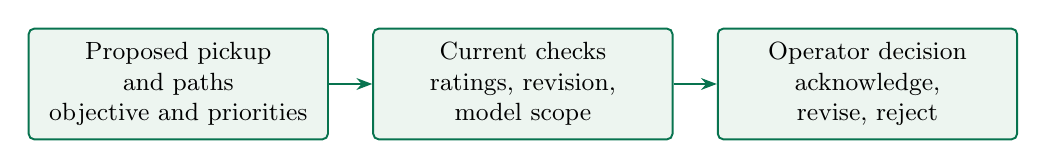
\begin{tikzpicture}[node distance=.55cm]
\node[box,text width=3.45cm] (a) {Proposed pickup and paths\\objective and priorities};
\node[box,text width=3.45cm,right=of a] (b) {Current checks\\ratings, revision, model scope};
\node[box,text width=3.45cm,right=of b] (c) {Operator decision\\acknowledge, revise, reject};
\draw[arrow] (a)--(b);\draw[arrow] (b)--(c);
\end{tikzpicture}
\end{center}
\Idea{A complete recommendation is conditional}{State which measurements and equipment statuses were trusted. A passing calculation is tied to that information and that model.}
\Question{What if the network model is correct but the measurements are deceptive?}
\Answer{The planner may optimize the wrong state. The next case tests consistency, observability and trusted replacement evidence.}
\Source{Restoration lessons: Classroom\_Labs L6--L7 and archived L10 trace. Operator acknowledgment is a tutorial workflow, not a field execution system.}
\Bridge{Can internally consistent measurements still describe the wrong state?}
\note{Close restoration with the operator's view. A recommendation should identify what demand is restored, what topology it assumes, the service priorities, the modeled limits and the evidence revision. It should also state what was not certified, especially switching sequence and protection behavior in these exercises. Acknowledgment is not merely clicking through a green badge; it is a decision made with those conditions visible. Participants have now seen two complementary benefits: an optimization objective that protects designated demand, and a workflow that prevents stale or failed evidence from being treated as valid. Neither requires claiming that Llama improves the optimum. Use the final question as the transition to cyber response. Even a correct network model and a competent optimizer can recommend the wrong action when measurements describe the wrong state. The next lesson separates consistency from trust.}
\end{frame}

\section{Cyber response: consistency and trustworthy evidence}
% Native, editable teaching diagrams. C01--C18; no AI-generated imagery.
\begin{frame}[t]{Sensors report numbers; the state is what we infer}
\label{f:C01}
\begin{columns}[T,onlytextwidth]
\column{.48\textwidth}
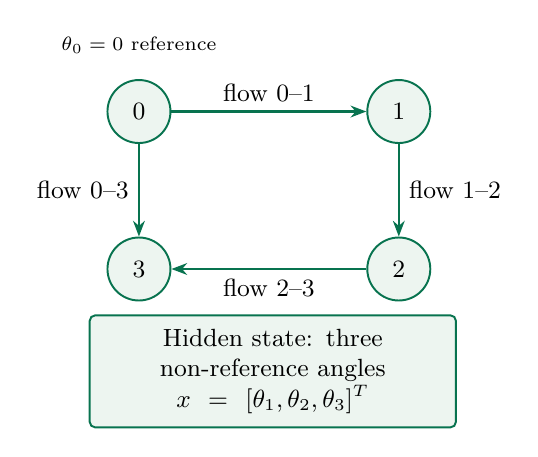
\begin{tikzpicture}[every node/.style={font=\small},x=1cm,y=1cm]
\node[circle,draw=teal,fill=pale,minimum size=8mm] (n0) at (0,1.8) {0};
\node[circle,draw=teal,fill=pale,minimum size=8mm] (n1) at (3.3,1.8) {1};
\node[circle,draw=teal,fill=pale,minimum size=8mm] (n2) at (3.3,-.2) {2};
\node[circle,draw=teal,fill=pale,minimum size=8mm] (n3) at (0,-.2) {3};
\draw[arrow] (n0)--node[above] {flow 0--1}(n1);
\draw[arrow] (n1)--node[right] {flow 1--2}(n2);
\draw[arrow] (n2)--node[below] {flow 2--3}(n3);
\draw[arrow] (n0)--node[left] {flow 0--3}(n3);
\node[font=\scriptsize,above=2mm of n0] {$\theta_0=0$ reference};
\uncover<2->{\node[box,text width=4.3cm] at (1.7,-1.5) {Hidden state: three non-reference angles\\$x=[\theta_1,\theta_2,\theta_3]^T$};}
\end{tikzpicture}
\column{.49\textwidth}
\Idea{Fresh four-bus DC fixture}{Eight measurements: four flows, three injections, one angle. Three unknown angles. Redundancy permits a consistency test.}
\Question{Is a small residual the same as a trustworthy state?}
\Answer{No. We will construct two different states with the same residual.}
\small This identifiable DC example is separate from the three-phase distribution-feeder models.
\end{columns}
\Source{Classroom\_Labs L8--L9; standard\_formulations.run\_wls\_demo. State estimation: \href{https://doi.org/10.1109/TPAS.1970.292678}{Schweppe and Wildes, 1970}.}
\Bridge{What does fitting a state mean in a two-sensor example?}
\note{Start by distinguishing the network state from the sensor readings. In this small DC example, the state consists of three voltage angles relative to the reference bus. Voltage magnitudes and reactive power are outside the model. The measurements include branch flows, nodal injections and one angle reading, so they provide more equations than unknowns. That redundancy makes it possible to ask whether the readings agree with one modeled state. The arrows define branch reference directions, not necessarily actual positive power flow. Do not begin with an attack mechanism. First establish what an ordinary estimator is trying to do and what its residual means. The next two-sensor example is a separate arithmetic illustration, intentionally much simpler than this four-bus model. It lets the audience predict the estimator output before seeing matrix notation.}
\end{frame}

\begin{frame}[t]{Two equally precise sensors: find their common explanation}
\label{f:C02}
\begin{center}
\begin{tikzpicture}[node distance=1.5cm]
\node[box] (a) {sensor 1\\9 units};
\node[box,right=of a,text width=3cm] (b) {one hidden quantity $x$\\best estimate?};
\node[box,right=of b] (c) {sensor 2\\11 units};
\draw[arrow] (a)--(b);\draw[arrow] (c)--(b);
\uncover<2->{\node[box,below=.7cm of b,text width=7.2cm] (d) {$\hat x=(9+11)/2=10$\\residuals: $r=[9-10,\;11-10]^T=[-1,1]^T$};\draw[arrow] (b)--(d);}
\end{tikzpicture}
\end{center}
\Question{What mismatch remains after choosing the best common value?}
\Answer{$J=(-1)^2+1^2=2$. A residual measures mismatch to the fitted model.}
\small Illustrative scalar example: $H=[1,1]^T$, unit variance for each sensor. This is WLS with equal weights, not the four-bus run.
\Source{Original arithmetic teaching example; least-squares principle: \href{https://doi.org/10.1109/TPAS.1970.292678}{Schweppe and Wildes, 1970}.}
\Bridge{How does one inconsistent reading change the fit?}
\note{Ask the audience for the best common explanation of nine and eleven before revealing ten. Assume both sensors measure the same scalar in the same units, with equal independent noise variances of one. Under squared-error fitting, the average minimizes the sum of the two squared discrepancies. A residual is the observed reading minus the reading predicted by the fitted state. The two residuals are minus one and plus one; their squared sum is two. Explain the hat notation as an estimate rather than a true value. No detection threshold is being claimed for this arithmetic example. Its purpose is to make the estimator and residual concrete. The actual classroom network has different measurement types and variances, which later require weighting so an angle discrepancy and a flow discrepancy are compared in their own noise scales.}
\end{frame}

\begin{frame}[t]{An isolated error increases disagreement between sensors}
\label{f:C03}
\begin{columns}[T,onlytextwidth]
\column{.48\textwidth}
\Idea{Before corruption}{$z=[9,11]^T$\par $\hat x=10$\par $r=[-1,1]^T$\par $J=2$.}
\column{.48\textwidth}
\Idea{Change only sensor 1}{$z'=[15,11]^T$\par Which common estimate fits best?}
\uncover<2->{\[
\hat x'=13,\quad r'=[2,-2]^T,\quad J'=8.
\]}
\end{columns}
\begin{center}
\begin{tikzpicture}[x=.7cm]
\draw[slate,->] (8,0)--(16,0);
\foreach \x in {9,10,11,13,15}{\draw (\x,.07)--(\x,-.07);\node[below,font=\small] at (\x,-.08) {\x};}
\fill[teal] (9,0) circle (2pt);\fill[teal] (11,0) circle (2pt);
\uncover<2->{\draw[arrow,red,bend left=35] (9,.1) to node[above,font=\small] {one reading moves} (15,.1);\fill[red] (15,0) circle (2pt);}
\end{tikzpicture}
\end{center}
\footnotesize A calibrated alarm signals model inconsistency; it does not identify an attacker.
\Source{Original scalar illustration, equal unit variances. Statistical alarm assumptions are introduced on C06.}
\Bridge{What if both readings move together?}
\note{Keep the true physical quantity conceptually unchanged while modifying only the first reported number. The new readings, fifteen and eleven, are best explained by thirteen. Their residuals are plus two and minus two, so the squared mismatch rises from two to eight. This provides an intuitive reason why redundant measurements can detect some kinds of corruption: the readings no longer agree with one another as well. Do not label this arithmetic result an actual alarm, because we have not chosen a statistical threshold for this example. A larger residual can also arise from a failed sensor, incorrect topology, poor calibration or an inadequate model. An alarm indicates inconsistency under assumptions, not malicious intent. Ask what happens if both readings are changed by the same amount. That prediction prepares the central limitation without requiring matrix algebra yet.}
\end{frame}

\begin{frame}[t]{Coordinated errors can preserve the same disagreement}
\label{f:C04}
\begin{center}
\begin{tabular}{lccc}
\toprule & Measurements & Fitted state & Residual\\\midrule
Original & $[9,11]^T$ & $10$ & $[-1,1]^T$\\
Both shifted by $+3$ & $[12,14]^T$ & $13$ & $[-1,1]^T$\\\bottomrule
\end{tabular}
\end{center}
\uncover<2->{\begin{center}\large Same residual statistic: $J'=J=2$.\par\smallskip Different inferred state: $\hat x'=\hat x+3$.\end{center}}
\Idea{Consistency is not authenticity}{Both readings fit a shifted state. Consistency alone cannot recover the missing truth.}
\Question{Does LLM voting add an independent measurement?}
\Answer{No. New physical evidence must come from outside the corrupted readings.}
\Source{Original scalar adaptation of the false-data-injection principle in \href{https://doi.org/10.1145/1653662.1653666}{Liu, Ning and Reiter, CCS 2009}.}
\Bridge{How does the same idea appear in network state estimation?}
\note{This is the explicit counterexample the audience should remember. Both sensors are shifted by three, so their best common explanation shifts from ten to thirteen. Their differences from that explanation remain minus one and plus one. The residual test therefore sees exactly the same mismatch even though the inferred state has changed. The example does not require the audience to accept a complicated security claim on faith; every number can be checked mentally. Explain that the attack succeeds within this illustration because both readings can be altered coherently and there is no trustworthy independent anchor. An additional language model examining the same observations does not create that anchor. A useful agentic workflow must recognize information limits, request appropriate evidence or hold the action. The network version follows the same geometry through the measurement matrix.}
\end{frame}

\begin{frame}[t]{Weighted least squares fits the measurement model}
\label{f:C05}
\[
z=Hx+e,\qquad
\hat x=\arg\min_x (z-Hx)^T R^{-1}(z-Hx),\qquad
R=\operatorname{diag}(\sigma_1^2,\ldots,\sigma_m^2).
\]
\begin{columns}[T,onlytextwidth]
\column{.48\textwidth}
\begin{tabular}{ll}
$z\in\mathbb R^m$ & sensor measurements\\
$x\in\mathbb R^n$ & unknown state\\
$H\in\mathbb R^{m\times n}$ & linear measurement map\\
$e$ & measurement noise\\
$\sigma_j$ & channel $j$ noise scale\\
$R$ & noise covariance
\end{tabular}
\column{.48\textwidth}
\Idea{Our fresh network run}{$m=8$, $n=3$, $\operatorname{rank}(H)=3$.\par Flow $\sigma=0.004$ p.u.; injection $0.006$ p.u.; angle $0.0005$ rad.}
\uncover<2->{\small Higher precision means larger weight. Each discrepancy is normalized by its own noise scale.}
\end{columns}
\Source{Classroom\_Labs L8; standard\_formulations.weighted\_least\_squares. WLS: \href{https://doi.org/10.1109/TPAS.1970.292678}{Schweppe and Wildes, 1970}.}
\Bridge{How large is too large for the residual?}
\note{Translate each symbol into an object the audience already understands. The measurement matrix predicts sensor readings from a candidate state. The estimator chooses the state that minimizes the weighted squared disagreement. The covariance describes uncertainty in each channel; the implementation assumes independent errors, so it is diagonal. A precise channel receives more weight because a small discrepancy there is more surprising. Different measurement types may have different physical units, which is why each residual is scaled by its own standard deviation. In the fresh four-bus exercise there are eight measurements and three identifiable unknown angles. The matrix has full column rank, so the linear weighted fit has a unique state estimate. These facts make the following residual degrees-of-freedom calculation meaningful. They do not establish trustworthy provenance for the measurements or correctness of the network topology.}
\end{frame}

\begin{frame}[t]{A residual alarm is a statistical test under stated assumptions}
\label{f:C06}
\[
r=z-H\hat x,\qquad J=r^TR^{-1}r,\qquad
J>\chi^2_{m-n,\,1-\alpha}\ \Longrightarrow\ \text{alarm}.
\]
\begin{columns}[T,onlytextwidth]
\column{.48\textwidth}
\Idea{Classroom calibration}{$m-n=8-3=5$ residual degrees of freedom.\par $\alpha=0.01$; threshold $\chi^2_{5,0.99}=15.0863$.}
\column{.48\textwidth}
\uncover<2->{\Idea{Interpretation requires assumptions}{Correct linear model; full column rank; stated independent Gaussian noise and covariance. $\alpha$ is the nominal false-alarm probability.}}
\end{columns}
\Question{Does ``no alarm'' mean ``safe to control''?}
\Answer{No. It means this test found no excessive model inconsistency. Provenance and operating limits remain separate checks.}
\Source{Residual test implementation: standard\_formulations.weighted\_least\_squares. State estimation foundations: \href{https://doi.org/10.1109/TPAS.1970.292678}{Schweppe and Wildes, 1970}.}
\Bridge{Why can a coordinated shift leave this statistic unchanged?}
\note{Define the residual before defining the test statistic. Each squared residual is normalized by its variance, producing a dimensionless sum. With a correct full-rank linear model and independent Gaussian errors of the stated covariance, the statistic follows a chi-square distribution with the number of measurements minus the number of estimated states degrees of freedom. Here that is five. A one-percent upper-tail threshold is about fifteen point zero nine. This is a calibration statement under assumptions, not a guarantee in an arbitrary real network. An alarm can reflect model error or ordinary sensor failure. Conversely, a missing alarm cannot establish that data are authentic. Ask participants to recall the two sensors shifted together. The next slide shows why that arithmetic example extends exactly to a family of coordinated changes in the linear network model.}
\end{frame}

\begin{frame}[t]{The cancellation is visible in three lines}
\label{f:C07}
\begin{align*}
\text{Coordinated measurement change:}\qquad z'&=z+Hc,\\[7pt]
\uncover<2->{\text{New WLS estimate:}\qquad\hat x'&=\hat x+c,}\\[7pt]
\uncover<3->{\text{New residual:}\qquad r'&=z+Hc-H(\hat x+c)=z-H\hat x=r.}
\end{align*}
\small $c\in\mathbb R^n$: chosen state shift; $a=Hc$: coordinated change to sensor readings. Therefore $J'=J$ with unchanged covariance.
\Idea{The assumptions are part of the result}{Full-rank linear WLS; correct knowledge of $H$; ability to alter the required unprotected channels. A protected channel can restrict feasible shifts.}
\Question{Which term disappears when we subtract the predicted measurements?}
\uncover<3->{\textcolor{teal}{The added $Hc$ cancels exactly.}}
\Source{False-data-injection construction: \href{https://doi.org/10.1145/1653662.1653666}{Liu, Ning and Reiter, CCS 2009}. Defensive four-bus exercise in L8.}
\Bridge{Can your experiment reproduce equal residuals but different state errors?}
\note{Reveal the three lines separately and pause before the last cancellation. The vector c is a change in the inferred state, and multiplying it by H produces the corresponding change in all modeled sensor readings. For full-rank linear weighted least squares with the same weights, adding this measurement change shifts the fitted state by c. Subtracting the new predicted readings removes the same added term, leaving the original residual. No mysterious failure of the numerical solver is involved; it solves the altered measurement problem correctly. State the attack assumptions instead of implying that every real system permits this construction. The exercise assumes knowledge of the model and control of all required unprotected readings. Protected independent channels can prevent some shifts from being consistent. The following experiment is confined to a synthetic educational DC model.}
\end{frame}

\begin{frame}[fragile,t]{Hands-on: sweep isolated and coordinated corruption}
\label{f:C08}
\Checkpoint{L8}{Seven minutes: run the full cell; compare residual and state-error plots.}
\lstinputlisting[style=python,firstline=1,lastline=5]{snippets/L8.py}
\begin{columns}[T,onlytextwidth]
\column{.48\textwidth}
\Idea{Predict first}{For a growing isolated bias, what happens to $J$? For a growing $Hc$ shift, what happens to $J$ and the state error?}
\column{.48\textwidth}
\uncover<2->{\Idea{Read two different quantities}{The residual is observable from measurements and the model. State error uses simulated truth and is an offline evaluation metric.}}
\end{columns}
\small The scale multiplies a synthetic perturbation. It is not an estimate of attack likelihood or real-world severity.
\Source{Exact excerpt: Classroom\_Labs L8 lines 1--5. Fixed synthetic seeds and attack directions in src/classroom\_labs.py and standard\_formulations.py.}
\Bridge{Which curve can an operator compute without knowing the truth?}
\note{Give participants the full seven minutes to run and inspect the experiment. The attack scale varies over five stated values for both isolated corruption and the coordinated Hc construction. Ask them to predict the two plots before looking at the table. Their explanation should distinguish a detector output from an evaluation metric. The residual statistic can be computed from the reported measurements and the assumed model. The norm of state error requires the true simulated state, which is available to us because this is an experiment. A real operator does not generally know that truth. Do not let the workflow use offline truth as if it were an available verification signal. Participants should record one example where no residual alarm occurs despite a changed inferred state, and explain why additional independent information would be required.}
\end{frame}

\begin{frame}[t]{Same residual does not imply the same state}
\label{f:C09}
\begin{center}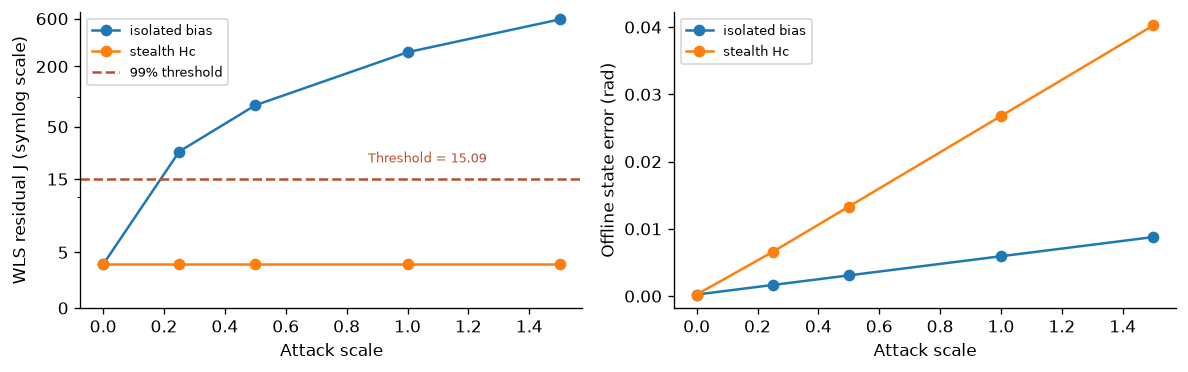
\includegraphics[width=.88\linewidth,height=3.65cm,keepaspectratio]{figures/classroom_cyber.png}\end{center}
\small At scale 1: isolated-corruption $J\approx277.50$; coordinated-shift $J\approx3.92$. Threshold $15.09$.
\uncover<2->{\Idea{Keep the metrics separate}{Left: consistency evidence available to the estimator. Right: state error against simulated truth, used only to evaluate the experiment.}}
\Source{Original computed figure: Classroom\_Labs L8 / classroom\_cyber.png. Coordinated $J\approx3.92022$ remains constant across the sampled scales.}
\Bridge{What should Awareness report when consistency passes but trust is unresolved?}
\note{Read the plots in order. The residual plot shows that a sufficiently large isolated perturbation violates the consistency test, while the coordinated construction retains the original statistic at every sampled scale. The state-error plot reveals that the coordinated corruption still changes the inferred state. Mention the residual-axis scaling shown on the figure so students do not interpret vertical distances as an ordinary linear scale. At scale one, the isolated statistic is about two hundred seventy-seven, well above fifteen, while the coordinated statistic remains about three point nine. Those are reproducible outcomes for the stated synthetic seeds and model, not general attack-detection rates. The right-hand plot is an offline scientific audit using known truth. The next workflow decision must instead rely on information actually available to the estimator and the declared provenance assumptions.}
\end{frame}

\begin{frame}[t]{Awareness must distinguish consistency from trustworthy provenance}
\label{f:C10}
\begin{center}
\begin{tikzpicture}[node distance=.65cm]
\node[box,text width=3.3cm] (a) {Residual test\\Do readings fit the model?};
\node[box,text width=3.3cm,right=of a] (b) {Provenance check\\Which channels are trusted?};
\node[box,text width=3.3cm,right=of b] (c) {Control decision\\Enough evidence to act?};
\draw[arrow] (a)--(b);\draw[arrow] (b)--(c);
\end{tikzpicture}
\end{center}
\Idea{A legitimate output is HOLD}{If measurements are suspect and no trustworthy replacement is available, request evidence instead of manufacturing a confident state estimate.}
\Question{Can an LLM vote resolve missing observability or missing trusted channels?}
\Answer{No. Voting over the same evidence does not add an independent physical constraint.}
\Source{Information limitation illustrated by \href{https://doi.org/10.1145/1653662.1653666}{Liu et al., 2009}; explicit protected-channel assumption in Classroom\_Labs L9.}
\Bridge{What replacement information is assumed in the recovery exercise?}
\note{This slide places the statistical lesson inside the agentic workflow. Awareness should produce separate fields for residual consistency and measurement provenance. A low residual supports only the first field. If a cyber incident or external evidence makes the measurements suspect, the workflow should ask whether trustworthy replacement channels exist and whether they make the state identifiable. The language model can summarize the missing evidence, request an authorized tool or explain why the action is held. It cannot create a trustworthy measurement by reasoning more fluently. Multiple model responses based on the same corrupted data have the same information limitation. The exercise deliberately includes a HOLD branch when replacement channels are unavailable. This is not a claim that the residual test itself detects the stealth case; that would contradict the counterexample we just demonstrated.}
\end{frame}

\begin{frame}[t]{Recovery assumes three independent protected angle readings}
\label{f:C11}
\[
z_T=H_Tx+e_T,\qquad H_T=I_3,\qquad
\sigma_T=0.00005\ \text{rad per channel}.
\]
\begin{center}
\begin{tikzpicture}[node distance=.65cm]
\node[box,text width=2.7cm] (a) {protected $\theta_1$};
\node[box,text width=2.7cm,right=of a] (b) {protected $\theta_2$};
\node[box,text width=2.7cm,right=of b] (c) {protected $\theta_3$};
\uncover<2->{\node[box,text width=8.2cm,below=.65cm of b] (d) {Rank 3: recover three angles.\\Exactly determined: zero residual degrees of freedom.};\draw[arrow] (a)--(d);\draw[arrow] (b)--(d);\draw[arrow] (c)--(d);}
\end{tikzpicture}
\end{center}
\small Subscript $T$: trusted set; $I_3$: identity matrix; $e_T$: assumed measurement noise.
\Idea{An assumption, not an implemented security protocol}{Authentication and physical protection are external requirements. This three-channel fit provides no redundant chi-square detection test.}
\Source{Exact classroom recovery model: standard\_formulations.run\_wls\_demo; Classroom\_Labs L9. Protected measurements are assumed trustworthy.}
\Bridge{How can a trusted estimate support a constrained corrective action?}
\note{Be explicit that the recovery channels are assumed, not discovered by the LLM or authenticated by this notebook. There are three independent angle readings, one for each unknown angle, with the stated small noise level. The identity measurement matrix has rank three, so the state is identifiable from this trusted set. However, three measurements for three unknowns leave zero residual degrees of freedom. The estimator can fit them exactly, so it has no redundant chi-square test for detecting an error within this set. Trust must come from the external measurement and security assumptions. This distinction prevents the recovery demonstration from becoming a circular claim that a zero residual proves security. Ask participants what additional engineering would be needed to establish that trust in practice. The tutorial then uses the recovered estimate for a small constrained redispatch calculation.}
\end{frame}

\begin{frame}[t]{Corrective control: move a stressed flow back inside its limit}
\label{f:C12}
\begin{columns}[T,onlytextwidth]
\column{.49\textwidth}
\begin{tikzpicture}[x=15cm,y=1cm]
\draw[slate,->] (0,0)--(.29,0);
\foreach \x in {.17,.18,.24}{\draw (\x,.1)--(\x,-.1);}
\node[font=\scriptsize,below] at (.24,-.12) {0.24};
\draw[slate] (.17,-.12)--(.12,-.45);
\node[font=\scriptsize,below] at (.12,-.45) {target 0.17};
\draw[red,dashed,thick] (.18,-.1)--(.18,1);
\node[font=\small,above] at (.18,1) {limit 0.18};
\fill[red] (.24,0) circle (2.4pt);
\uncover<2->{\draw[arrow,bend right=25] (.24,.15) to node[above,font=\small] {flexible injection $u$} (.17,.15);\fill[teal] (.17,0) circle (2.4pt);}
\end{tikzpicture}
\column{.48\textwidth}
\Idea{Noiseless arithmetic illustration}{For branch 1--2, suppose estimated flow is $0.24$ p.u. and sensitivity is $-4/7$.\par A $0.01$ p.u. margin gives target $0.17$.\par\smallskip $u\ge(0.24-0.17)/(4/7)=0.1225$ p.u.}
\end{columns}
\small $u$: injection at node 2, balanced by the reference source. The actual noisy protected-state run gives $u\approx0.12169$ p.u.; the illustration above is not that exact solve.
\Source{Sensitivity $F B^{-1}[0,1,0]^T$ from standard\_formulations.\_redispatch. Original noiseless arithmetic illustration; all quantities here are per unit.}
\Bridge{How do we choose the smallest admissible correction across all branches?}
\note{Before showing a quadratic program, make the control action concrete. An injection at node two, balanced by the reference source, changes branch flows through a known DC sensitivity. For the stressed branch, the sensitivity is minus four-sevenths. In this separate noiseless illustration, an estimated flow of zero point two four must be brought to zero point one seven to preserve a zero point zero one margin below the physical zero point one eight limit. Dividing the needed flow reduction by the sensitivity magnitude gives a minimum injection of zero point one two two five. The real classroom solve uses a noisy protected estimate, so its optimum is slightly different. Label that distinction carefully. The diagram does not use simulated truth as an operational gate; it simply teaches how a linear flow sensitivity becomes an action constraint.}
\end{frame}

\begin{frame}[fragile,t]{Planning uses a constrained quadratic control problem}
\label{f:C13}
\[
\min_{0\le u\le0.5}\ \tfrac12u^2
\quad\text{s.t.}\quad
\left|F\hat x_T+b_u u\right|\le\ell-\delta\mathbf1,
\qquad b_u=FB^{-1}e_2.
\]
\small
$F$: angle-to-flow map; $B$: non-reference nodal injection matrix; $e_2=[0,1,0]^T$; $\hat x_T$: trusted estimate; $b_u$: flow sensitivity.\par
$\ell=[0.35,0.18,0.35,0.35]^T$ p.u.: branch limits; $\delta=0.01$ p.u.: planning margin; $\mathbf1$: vector of ones. Absolute values and inequalities are componentwise.
\Checkpoint{L9}{Run both evidence conditions with the same numerical control method.}
\lstinputlisting[style=python,firstline=1,lastline=2]{snippets/L9.py}
\uncover<2->{\Idea{Method and acceptance}{SLSQP solves this scalar convex QP. Independent post-solve bounds and predicted-flow checks can still return HOLD.}}
\Source{Exact excerpt: Classroom\_Labs L9 lines 1--2; constrained model and checks in standard\_formulations.\_redispatch. DC illustration, not AC feeder resilience.}
\Bridge{What changes when trusted replacement channels are unavailable?}
\note{Read the objective as choosing the smallest squared corrective injection. The constraints keep all predicted branch-flow magnitudes within their ratings minus the engineering margin, and restrict the injection to its allowed interval. Define every matrix by its role instead of asking students to memorize the notation. The vector e-two selects injection at the second non-reference node, while the reference source balances the change. For this fixed linear model, the resulting scalar problem is convex. The implementation uses SLSQP and independently checks finite values, action bounds and predicted flow constraints after solving. The protected estimate is an input with an explicit trust assumption. The two code lines compare that assumption being available or unavailable; they do not change the numerical control objective. This distinguishes an information gate from a contest between optimization algorithms.}
\end{frame}

\begin{frame}[t]{Hands-on: evidence availability changes the permitted response}
\label{f:C14}
\Checkpoint{L9}{Five minutes: run the full cell; identify the acceptance assumption.}
\begin{center}
\begin{tabular}{lcc}
\toprule Condition & Response & Flexible injection\\\midrule
No trusted replacement channels & HOLD & none proposed\\
Three protected angles assumed & PROPOSE & $0.12169$ p.u.\\\bottomrule
\end{tabular}
\end{center}
\uncover<2->{\Idea{Two checks, with different information}{Predicted branch 1--2 flow: $0.17000$ p.u. (operational model check).\par Actual simulated flow: $0.17046<0.18$ p.u. (offline truth audit).}}
\Question{Why is the offline value not an input to the operator's verification rule?}
\Answer{The real system does not reveal its exact state just because our simulator knows it.}
\Source{Fresh L9 output with fixed synthetic seeds; standard\_formulations.run\_wls\_demo. The zero-violation offline audit applies to this modeled case only.}
\Bridge{How does the five-stage workflow carry this distinction?}
\note{Allow five minutes for the full cell and discussion. The no-trust condition returns HOLD rather than an invented replacement state. The protected condition proposes a flexible injection of about zero point one two one six nine per unit. The predicted stressed-branch flow is at the zero point one seven planning target. When the experiment separately evaluates that same action against its known true state, the actual modeled flow is about zero point one seven zero four six, still below the physical limit. These numbers have different roles. Predicted constraints support the candidate under the trusted-estimate assumption. Truth-based flow and violation count are offline performance audits. A successful audit on one seeded example is not a robustness guarantee against arbitrary measurement error or model mismatch. Ask participants to state the protected-channel assumption in their own words before moving on.}
\end{frame}

\begin{frame}[t]{Every stage has a specific numerical or evidentiary job}
\label{f:C15}
\small
\renewcommand{\arraystretch}{1.12}
\begin{tabularx}{\linewidth}{>{\bfseries\raggedright\arraybackslash}p{2.35cm}>{\raggedright\arraybackslash}p{4.4cm}>{\raggedright\arraybackslash}X}
\toprule Stage & Specific method & Inspectable output\\\midrule
Awareness & WLS, residual and trust checks & Alarm, rank, provenance status\\
Planning & Constrained DC redispatch QP & Injection and predicted flow margins\\
Simulation & DC flow calculation & Response to the candidate injection\\
Verification & Provenance and limit gates & PROPOSE or HOLD, with failed condition\\
LLM Optimizer & Allowed refinement selection & New tool request and returned rationale\\\bottomrule
\end{tabularx}
\uncover<2->{\Idea{Use the method suited to the decision}{WLS estimates the state; the QP selects the correction. L10 replays the archived five-stage language trace.}}
\Source{Classroom\_Labs L8--L10; archived cyber\_stealth / dc run in proposal\_complete\_workflow.json. Fresh numerical fixtures and archived LLM calls are separately labeled.}
\Bridge{What does the actual Llama refinement response look like?}
\note{Return to the five-stage vocabulary after the audience understands the numerical problem. Awareness computes an estimate and a consistency statistic, but also records rank and trust conditions. Planning solves the constrained redispatch problem only when its required inputs are admissible. Simulation evaluates the action in the stated DC model. Verification checks provenance and modeled limits and can hold the recommendation. The language optimizer may select from permitted refinements and request another simulation; it cannot waive those gates. This case uses a quadratic program because that is the natural form of the stated decision. It would be misleading to label every calculation MPC or DRL for consistency of branding. L8 and L9 are fresh numerical exercises, while L10 supplies the full archived language trace. That distinction keeps live execution, replayed evidence and conceptual stage roles honest.}
\end{frame}

\begin{frame}[t]{Actual Llama response: request a new checked candidate}
\label{f:C16}
\small
\Idea{Planning, 0.829 s}{\textit{``Requesting new candidates based on the given tools and objective.''}}
\uncover<2->{\Idea{LLM Optimizer selects TRUSTED\_QP, 1.195 s}{\textit{``The current lowest-cost candidate E03 has a cost of 0.008671610999497877, but the permitted refinement TRUSTED\_QP offers a new approach to minimize the objective. Selecting this operation will request a new simulation and verification.''}}}
\uncover<3->{\begin{center}\textbf{Numerical result:} $u=0.12169$ p.u., cost $0.00740467$.\par Acceptance still depends on trusted-input and flow-limit gates.\end{center}}
\Source{Exact returned rationale fields: archived cyber\_stealth / dc trace, proposal\_complete\_workflow.json. Model-call wall times; rounded only outside quotes.}
\Bridge{Does this language-guided refinement outperform the matched fixed supervisor?}
\note{Present these as observable response fields from the saved trace, not as access to hidden internal reasoning. The short planning reply requests candidates. The optimizer reply selects a permitted trusted-QP refinement and explicitly asks for another simulation and verification. The reported model-call times are about eight hundred twenty-nine milliseconds and one point one nine five seconds in the archived environment. The final numerical result comes from the constrained solver and its checks, not from the prose. The response does not prove that the trusted measurements are authentic, that the DC model is adequate for a distribution feeder, or that an operator has authorized execution. Those remain separate conditions. This example shows where a language response can help explain a workflow step while leaving authority with defined tools, evidence and approval. The next slide tests the final outcome against the fixed supervisor.}
\end{frame}

\begin{frame}[t]{A matched baseline avoids crediting the LLM for better information}
\label{f:C17}
\begin{center}
\begin{tabular}{lrr}
\toprule Archived DC cyber response & Fixed supervisor & Llama supervisor\\\midrule
Flexible injection (p.u.) & 0.12169 & 0.12169\\
Objective $\tfrac12u^2$ & 0.00740467 & 0.00740467\\
Total elapsed time (s) & 0.00381 & 5.203\\\bottomrule
\end{tabular}
\end{center}
\uncover<2->{\Idea{What actually enabled recovery?}{The trusted measurement assumption plus constrained numerical control. Llama added tool-selection language and a trace; it did not improve this recorded optimum.}}
\Question{Would comparing untrusted baseline data with trusted agent data be fair?}
\Answer{No. That would mix the value of additional information with the value of orchestration.}
\Source{ARCHIVED ACTUAL: fixed versus agentic cyber\_stealth / dc, proposal\_complete\_workflow.json. Same objective and evidence assumptions; one recorded run, four Llama calls.}
\Bridge{What should the operator see when the workflow finishes?}
\note{The fixed and Llama supervisors reach the same action and objective in this archived DC case. Their total elapsed times differ substantially, with the fixed supervisor completing in a few milliseconds and the language-guided workflow taking about five seconds. These are single-run measurements, not distributions or universal performance claims. The comparison is meaningful because the numerical objective, tools and evidence assumptions are matched. If the baseline had only corrupted measurements while the agent received protected measurements, any benefit would combine better information with orchestration. Avoid making that unfair attribution. The scientific lesson is that protected information and constrained control enable the recovery in this example. The agentic layer can organize requests, reasons, holds and evidence, but its additional value should be evaluated through explicit workflow and human-performance measures, alongside its latency and failure modes.}
\end{frame}

\begin{frame}[t]{The control-room handoff is a decision packet, not a green badge}
\label{f:C18}
\begin{columns}[T,onlytextwidth]
\column{.49\textwidth}
\Idea{What the operator sees}{Proposed action and objective.\par Sensor trust and model scope.\par Current revision and failed/passed checks.\par Measured latency and available alternatives.}
\column{.47\textwidth}
\begin{tikzpicture}[node distance=.55cm]
\node[box,text width=4.3cm] (a) {Evidence-backed recommendation};
\node[box,text width=4.3cm,below=of a] (b) {Acknowledge \quad Revise \quad Reject};
\node[box,text width=4.3cm,below=of b] (c) {Read back the resulting state};
\draw[arrow] (a)--(b);\draw[arrow] (b)--(c);
\end{tikzpicture}
\end{columns}
\Question{What did the three cases teach about choosing numerical methods?}
\Answer{Continuous voltage control, discrete restoration and evidence-limited cyber response need different tools within one auditable workflow.}
\Source{Case synthesis: Classroom\_Labs L1--L10; operator readback exercise L12. The tutorial dashboard is an educational interface, not a deployed control system.}
\Bridge{How should we evaluate usefulness, reliability and operator effort together?}
\note{End the cyber chapter by returning to the operator rather than to an optimizer score. A useful recommendation includes its proposed action, the objective, the measurement trust assumptions, the model used, the relevant revision and the outcome of each required check. The operator can then acknowledge, revise or reject it. After any authorized action, readback should establish what state was actually reached; an acknowledgment alone is not physical confirmation. Across the three cases, the numerical tools differ because the decisions differ. Voltage support uses continuous-control methods, restoration adds discrete topology and pickup choices, and cyber response exposes information and provenance limits before constrained control. The common agentic framework is a disciplined flow of requests, tools, checks and human decisions. The closing section will evaluate that workflow without confusing documentation quality with electrical performance or claiming unmeasured benefits.}
\end{frame}

\section{Evaluation and operator decisions}
\begin{frame}[t]{What did the framework actually improve?}\label{f:E01}
\begin{columns}[T]\column{.47\textwidth}\centering\begin{tikzpicture}[x=1cm,y=1cm]
\node[box,text width=3.9cm] (n) at (0,2.4) {\textbf{Numerical question}\\Did the action satisfy the stated electrical limits?};
\node[box,text width=3.9cm] (w) at (0,.6) {\textbf{Workflow question}\\Was the right study run and attached to this action?};
\node[box,text width=3.9cm] (h) at (0,-1.2) {\textbf{Operator question}\\Can a reviewer identify the action and its remaining uncertainty?};
\end{tikzpicture}\column{.50\textwidth}
\textbf{Measure the workflow and the electrical outcome separately.}\par\medskip
\begin{itemize}\item Study completed?\item Constraints passed?\item Claims supported?\end{itemize}
\Question{Which claim is supported by a low cost and a fluent explanation?}
\end{columns}
\Source{\href{https://arxiv.org/html/2606.18789v1}{PowerAgentBench-SS (2026), \S{}\S{}II--III}; \href{../Classroom_Labs.html}{Executed tutorial: Classroom\_Labs, L0--L12}}
\Bridge{Compare methods on the same task}
\note{Ask learners to answer this using one case they just ran. A study can finish while its candidate is infeasible. A rejected candidate can demonstrate a working gate while consuming time. A numerical improvement can come from a stronger optimizer rather than the LLM. Put those observations in different columns. The tutorial establishes an executable learning workflow with visible intermediate decisions; it does not yet establish a benefit in a utility control room. Invite the audience to name the smallest extra experiment needed for their preferred claim. A claim about staff workload requires participants and a workload measure. A claim about electrical feasibility requires a stated model, operating limits and test scenarios. Transition: make the comparison fair before interpreting any score.}
\end{frame}

\begin{frame}[t]{Compare methods on the same task}\label{f:E02}
\begin{columns}[T]\column{.47\textwidth}\centering\begin{tikzpicture}[x=1cm,y=1cm]
\node[box,text width=3.2cm] (c) at (0,2.3) {One scenario\\same measurements and limits};
\node[box,text width=1.7cm] (a) at (-1.35,.5) {Fixed controller};
\node[box,text width=1.7cm] (b) at (1.35,.5) {Agentic workflow};
\node[box,text width=3.3cm] (v) at (0,-1.3) {Same final verifier\\compare feasibility first};
\draw[arrow] (c)--(a);\draw[arrow] (c)--(b);\draw[arrow] (a)--(v);\draw[arrow] (b)--(v);
\end{tikzpicture}\column{.50\textwidth}
\textbf{Give every method the same physical constraints and verification budget.}\par\medskip
For case $i$, record whether every constraint passes.\[\widehat p=\frac{1}{N}\sum_{i=1}^{N}\mathbf1[\text{all checks pass}]\] $N$ is the number of cases. If 8 of 10 pass, $\widehat p=0.8$. This arithmetic example is illustrative.\par\medskip
\begin{itemize}\item Same case and admissible actions\item Same candidate trial budget\item Same final verifier\end{itemize}
\end{columns}
\Source{\href{https://arxiv.org/html/2606.18789v1}{PowerAgentBench-SS (2026), \S{}\S{}II--III}; \href{../LLM_Response_Selection.html}{Recorded voltage pilot: E1--E8}}
\Bridge{Ablate one mechanism at a time}
\note{Use the same demand realization, topology, operating limits, action bounds and final electrical check for a paired comparison. A method that sees more cases or gets extra simulations has received additional information or compute. Record that explicitly. The fixed baseline may use the same MPC, SAC policy and verifier as the agentic workflow; this isolates orchestration rather than changing the entire controller. Report the objective among feasible candidates and also report the failure fraction. An average objective that silently removes failed cases can favor a brittle method. In the held-out response pilot, all pool selectors paid for all three LLM calls. The learned selector therefore cannot claim the latency of only the chosen response. Transition: choose the ablation that answers the claim.}
\end{frame}

\begin{frame}[t]{Ablate one mechanism at a time}\label{f:E03}
\begin{columns}[T]\column{.47\textwidth}\centering\begin{tikzpicture}[x=1cm,y=1cm]
\node[box,text width=3.6cm] (a) at (0,2.3) {MPC + fixed numerical checks};
\node[box,text width=3.6cm] (b) at (0,.9) {Same tools + LLM proposals};
\node[box,text width=3.6cm] (c) at (0,-.5) {Same proposals + selector};
\draw[arrow] (a)--node[right,font=\scriptsize]{change one mechanism}(b);
\draw[arrow] (b)--node[right,font=\scriptsize]{keep the trial budget fixed}(c);
\end{tikzpicture}\column{.50\textwidth}
\textbf{A useful ablation keeps the numerical tools fixed.}\par\medskip
\begin{itemize}\item Fixed numerical workflow\item Add language interpretation\item Add role-specific handoffs\end{itemize}
\end{columns}
\Source{\href{https://arxiv.org/html/2606.18789v1}{PowerAgentBench-SS (2026), \S{}\S{}II--III}; \href{../Graph_Workflow_Lab.html}{Executed LangGraph teaching lab: G0--G5}; \href{../LLM_Response_Selection.html}{Recorded voltage pilot: E1--E8}}
\Bridge{Frontier: evidence-backed evaluation}
\note{Build the comparison from left to right. First establish a deterministic workflow that solves the engineering problem. Add language interpretation while preserving its tool contract. Then introduce specialist handoffs and measure whether they reduce malformed requests or unsupported reports on varied tasks. Finally compare selection rules under the same candidate pool and fresh-trial budget. This is a recommended experimental design, not a claim that every ablation was run in this package. The implemented pilot directly compares several response selectors and fixed numerical refinement; the real LangGraph exercise separately checks orchestration equivalence against direct Python. Keep those scopes visible. Ask which variant would isolate the value of retrieval or a checkpoint. Transition: a recent benchmark formalizes this separation between tools and scoring.}
\end{frame}

\begin{frame}[t]{Frontier: evidence-backed evaluation}\label{f:E04}
\begin{columns}[T]\column{.47\textwidth}\centering\begin{tikzpicture}[x=1cm,y=1cm]
\node[box,text width=3.5cm] (a) at (0,2.3) {Agent-visible tools\\case, constraints, tool results};
\node[box,text width=3.5cm] (b) at (0,.7) {Submitted recommendation\\action + supporting records};
\draw[dashed,red] (-2.4,-.2)--(2.4,-.2) node[right,font=\scriptsize]{boundary};
\node[box,text width=3.5cm,draw=red] (c) at (0,-1.2) {Independent evaluation\\hidden physical revalidation};
\draw[arrow] (a)--(b);\draw[arrow] (b)--(c);
\end{tikzpicture}\column{.50\textwidth}
\textbf{The final report should survive independent recomputation.}\par\medskip
\begin{itemize}\item \checkmark Public tools and fixed budgets\item \checkmark Hidden physical revalidation\item \checkmark Evidence-supported submissions\end{itemize}
\end{columns}
\Source{\href{https://arxiv.org/html/2606.18789v1}{PowerAgentBench-SS (2026), \S{}\S{}II--III}}
\Bridge{Frontier: request uncertainty studies}
\note{PowerAgentBench-SS separates an agent-visible tool environment from hidden evaluation. Its instantiated pilot studies DC thermal contingency analysis, so it is useful here as an evaluation pattern rather than evidence for our voltage controller. For the classroom, draw a boundary around what the agent may observe and place the final scoring calculation outside it. Training feedback and selector features must not contain the held-out answer. A correct statement can still lack supporting evidence in the submitted trace, which is why claim support deserves its own measure. Have a learner point to the tool record supporting one numerical sentence in an operator report. If the record is absent, mark the sentence unsupported even if its value happens to be true. Transition: operating uncertainty is another dimension the workflow must expose.}
\end{frame}

\begin{frame}[t]{Frontier: request uncertainty studies}\label{f:E05}
\begin{columns}[T]\column{.47\textwidth}\centering\begin{tikzpicture}[x=1cm,y=1cm]
\node[box,text width=2.6cm] (a) at (0,2.5) {One proposed action};
\foreach \x/\v/\i in {-1.6/0.9/1,0/1.0/2,1.6/1.1/3}{\node[box,text width=1cm,font=\scriptsize] (n\i) at (\x,.7) {Load\\$\v d$};\draw[arrow] (a)--(n\i);}
\node[box,text width=3.5cm] (b) at (0,-1.2) {Inspect voltage and current in every scenario};
\foreach \i in {1,2,3}{\draw[arrow] (n\i)--(b);}
\end{tikzpicture}\column{.50\textwidth}
\textbf{The orchestrator can request a stronger study when uncertainty matters.}\par\medskip
Illustrative sensitivity study: use base demand $d$ and two nearby load levels. Keep the same action in all three trials.\par\medskip
\begin{itemize}\item \checkmark Numerical engines remain explicit\item \checkmark Uncertainty-aware study selection\item \checkmark Corrective-dispatch tools\end{itemize}
\end{columns}
\Source{\href{https://arxiv.org/html/2606.24609v1}{CONDUCTOR (2026), uncertainty-aware orchestration}; \href{../Classroom_Labs.html}{Executed tutorial: Classroom\_Labs, L0--L12}}
\Bridge{Frontier: enforce authority in software}
\note{CONDUCTOR provides a recent example of language orchestration around numerical grid-analysis engines, including uncertainty-aware analysis. Its reported measurement replay must not be described as a forecast-performance experiment. Relate that distinction to our load-scale exercise: changing a scenario is a sensitivity study, while a probability claim needs a justified distribution and calibration. A useful extension is to provide a small declared scenario set, run the same candidate through every scenario, and summarize the observed margins. That extension is proposed here; it is not an experiment already contained in the saved classroom output. Ask what additional data would justify the chosen scenarios for a real feeder. Transition: uncertainty about the grid and authority to act are separate concerns.}
\end{frame}

\begin{frame}[t]{Frontier: enforce authority in software}\label{f:E06}
\begin{columns}[T]\column{.47\textwidth}\centering\begin{tikzpicture}[x=1cm,y=1cm]
\node[box,text width=3.4cm] (p) at (0,2.5) {Proposed action};
\node[box,text width=3.4cm] (g) at (0,.9) {Software checks\\scope, identity, permission};
\node[box,text width=1.6cm] (r) at (-1.35,-1.1) {Eligible for review};
\node[box,text width=1.6cm,draw=red] (s) at (1.35,-1.1) {HOLD with reason};
\draw[arrow](p)--(g);\draw[arrow](g)--node[left,font=\scriptsize]{pass}(r);\draw[arrow](g)--node[right,font=\scriptsize]{fail}(s);
\end{tikzpicture}\column{.50\textwidth}
\textbf{Approval rules belong in the runtime, not only in the prompt.}\par\medskip
\begin{itemize}\item \checkmark Whitelisted tools\item \checkmark Explicit step budgets\item \checkmark Typed numerical facts\end{itemize}
\end{columns}
\Source{\href{https://arxiv.org/html/2609.22476v1}{Governance-aware TSO digital twin (2026)}; \href{../Classroom_Labs.html}{Executed tutorial: Classroom\_Labs, L0--L12}}
\Bridge{L11: one optional local Llama call}
\note{The governance-aware TSO digital-twin paper uses an external control layer for tool permissions, budgets and approval. Its reported prototype distinguishes task success from compliance with those enforced rules. Bring that distinction into our notebook: a candidate can satisfy the advisory readback rule without becoming a field command. Conversely, a plausible language answer cannot make an unavailable permission appear. Draw the authorized path through the review gate and show the attempted bypass ending at HOLD. This is an architectural lesson, not a claim of production certification. Ask learners to identify which checks run outside the language model in L12. The answer includes candidate identity, evidence binding and required model scope. Transition: now test what the existing experiments actually support.}
\end{frame}

\begin{frame}[t]{L11: one optional local Llama call}\label{f:E07}
\Checkpoint{L11}{Exact notebook excerpt; run the complete cell in order.}
\Code{E07.py}
\Idea{Actual saved public response from Llama 3.1:8b}{``has the potential to reduce reactive effort magnitude by ten percent, which may improve the cost.''}
\uncover<2->{\textbf{Interpretation:} this proposes an allowed trial. The new numerical check decides whether the change is feasible and useful.}
\par\smallskip Enable \texttt{RUN\_LOCAL\_LLAMA=True} for a new call. The saved response remains available if the local service is slow.\Source{\href{https://docs.ollama.com/api/chat}{Ollama chat API}; \href{../Classroom_Labs.html}{Classroom L11 and saved actual validation}}
\Bridge{Where did one Llama call spend its time?}
\note{Run the complete L11 cell after the earlier engineering cells. Its default branch prints that no new model call occurred. The optional path requires RUN\_LOCAL\_LLAMA=True in L0 and a prepared local Ollama service containing llama3.1:8b. It asks for a choice from the bounded catalog on the original test\_01 context, then writes the actual response to a new journal. Do not silently apply that response to a modified classroom case. The quoted public reason comes from the separate 17 October validation and is a saved actual output, not a new live response generated by these slides. It proposes reducing reactive effort and uses cautious language about possible cost improvement. A fresh numerical trial is still required. Transition: inspect where the measured call spent its time.}
\end{frame}

\begin{frame}[t]{Where did one Llama call spend its time?}\label{f:E08}
\begin{columns}[T]\column{.62\textwidth}
\begin{tikzpicture}\begin{axis}[width=8.2cm,height=4.4cm,xbar,xmin=0,xmax=19,ytick={1,2,3,4},yticklabels={Other,Generation,Prompt processing,Model loading},xlabel={Seconds},nodes near coords,nodes near coords align={horizontal},every node near coord/.append style={font=\scriptsize},bar width=12pt,axis lines=left,xtick={0,5,10,15},enlarge y limits=.25,yticklabel style={font=\scriptsize}]
\addplot[fill=teal!70,draw=teal] coordinates {(.0378,1)(1.916,2)(15.192,3)(16.967,4)};
\end{axis}\end{tikzpicture}
\column{.35\textwidth}\textbf{Actual local Llama call}\par
Client elapsed time: \textbf{34.113 s}.\par\medskip
1,891 prompt tokens; 137 generated tokens.\par\medskip
Most time came before token generation. A warm repeat can behave differently.\par\medskip
\textbf{Do not call a replay ``inference latency''.}
\end{columns}\Source{\href{https://docs.ollama.com/api/chat}{Ollama chat API: timing fields}; \href{../Classroom_Labs.html}{Executed tutorial: Classroom\_Labs, L0--L12}}
\Bridge{Place the assistant beside the control-room tools}
\note{This is the saved actual Llama 3.1 8B call from the optional classroom validation, not a new call made by the slide. Ollama reports its loading, prompt-processing and generation durations; the client timer includes the complete request. Small differences include server and transport overhead, so do not force the components to equal the client total exactly. The response chose RELAX\_Q\_10\_PERCENT on the original test\_01 context and requested a newly checked trial; it did not certify that future trial. Warm loading, prompt length and hardware can change latency substantially. Ask the audience whether this call belongs in a subsecond control loop or an advisory study. A deadline claim would require repeated end-to-end measurements, including failures and fallback. Transition: present this evidence in an operator-facing packet.}
\end{frame}

\begin{frame}[t]{How the workflow could fit beside control-room tools}\label{f:O01}
\centering\begin{tikzpicture}[x=1cm,y=1cm]
\node[box,text width=2.7cm] (d) at (-4.6,1.4) {Existing control-room data\\measurements + topology};
\node[box,text width=2.7cm] (s) at (0,1.4) {Advisory study workspace\\MPC, SAC, simulation, checks};
\node[box,text width=2.7cm] (o) at (4.6,1.4) {Operator workstation\\action, evidence, unresolved issues};
\draw[arrow] (d)--node[above,font=\scriptsize]{read}(s);\draw[arrow](s)--node[above,font=\scriptsize]{report}(o);
\node[box,text width=3.4cm,draw=slate,fill=white] (a) at (4.6,-1.4) {Existing authorized dispatch process\\outside this tutorial};
\draw[dashed,thick,slate](o)--node[right,font=\scriptsize]{separate authority}(a);
\node[text width=6.9cm,align=left] at (-2.5,-1.1) {The assistant assembles an engineering recommendation. A human reviews the evidence in the context of operating procedures.};
\end{tikzpicture}
\par\medskip The tutorial is an advisory sandbox with an explicit human boundary.
\Source{\href{https://arxiv.org/html/2609.22476v1}{Governance-aware TSO digital twin (2026)}; \href{../Classroom_Labs.html}{Executed tutorial: Classroom\_Labs, L0--L12}}
\Bridge{Which existing systems supply the study?}
\note{Follow the data path from the existing operational applications to a read-only study context, then through numerical candidates and verification to a reviewable recommendation. This is a deployment concept. The notebooks use a synthetic feeder and teaching cases; they do not connect to a live control system. The diagram should make the human review point prominent without suggesting that a dashboard alone establishes useful human oversight. An operator needs the relevant evidence at the right time and must be able to reject or request clarification. Ask which information belongs in a structured field rather than generated prose: equipment identifiers, limits, model scope and candidate identity are strong examples. Transition: trace the operational inputs, then rehearse each case before inspecting the review packet.}
\end{frame}

\newcommand{\OperatorIdea}[2]{\par\smallskip\begin{beamercolorbox}[sep=4pt,wd=\linewidth]{block body}{\fontsize{9}{10.5}\selectfont\color{teal}\bfseries #1\par}\smallskip{\fontsize{9}{10.5}\selectfont #2\par}\end{beamercolorbox}\smallskip}
\begin{frame}[t]{The study starts with a consistent operating snapshot}\label{f:D01}
\hyphenpenalty=10000\exhyphenpenalty=10000
\fontsize{9}{10.5}\selectfont\raggedright
\centering
\begin{tikzpicture}[x=1cm,y=1cm,scale=.84,transform shape]
\node[box,text width=3.1cm] (a) at (-4.8,2.1) {SCADA / ADMS\\measurements, switch status};
\node[box,text width=3.1cm] (b) at (-4.8,.55) {GIS / OMS\\assets and outages};
\node[box,text width=3.1cm] (c) at (-4.8,-1) {DERMS / forecasts\\available DER, expected load};
\uncover<2->{\node[box,text width=3.2cm] (s) at (0,.55) {Validated study snapshot\\time + quality flags\\revision + units};
\draw[arrow](a.east)--++(.4,0)|-(s.north west);\draw[arrow](b)--(s);\draw[arrow](c.east)--++(.4,0)|-(s.south west);}
\uncover<3->{\node[box,text width=3.1cm] (r) at (4.8,.55) {Awareness agent\\bind operator request\\to this snapshot};\draw[arrow](s)--(r);}
\end{tikzpicture}
\par\smallskip\fontsize{8}{9.2}\selectfont SCADA: supervisory control and data acquisition; ADMS: advanced distribution management system.\\
GIS: geographic information system; OMS: outage management system; DERMS: distributed energy resource management system.
\Question{What if the switch status and model describe different network revisions?}
\Answer{Hold the study and reconcile the snapshot before calculating a recommendation.}
\Source{Proposed integration, not implemented live. \href{https://www.nlr.gov/grid/adms-test-bed}{NLR ADMS Test Bed}; tutorial L1 and L7 demonstrate input/evidence binding.}
\Bridge{How do the notebook functions become services?}
\note{Begin with the systems an operator already uses. SCADA and an ADMS provide operational measurements and equipment status. A geographic information system supplies asset and connectivity information, while an outage management system supplies outage context. A DER management system can provide controllable resource availability. The diagram is a proposed interface pattern, not a claim that these systems are connected to the tutorial. Each utility has its own system boundaries and authoritative records. The first engineering task is to reconcile identifiers, units, timestamps, quality flags and topology into one study snapshot. A language model cannot resolve contradictory physical status by choosing a plausible sentence. L1 and L7 illustrate the narrower input-binding mechanism. For a live deployment, authentication, source integrity, clock handling and model maintenance are additional work. Ask the audience which system is authoritative for switch status in their organization.}
\end{frame}

\begin{frame}[t]{The assistant runs beside the existing control system}\label{f:D02}
\hyphenpenalty=10000\exhyphenpenalty=10000
\fontsize{9}{10.5}\selectfont\raggedright
\centering
\begin{tikzpicture}[x=1cm,y=1cm,scale=.94,transform shape]
\node[box,text width=2.8cm] (input) at (-4.9,1.8) {Read-only data adapter\\validated snapshot};
\node[box,text width=3.1cm] (flow) at (0,1.8) {Workflow service\\typed state, bounded routing};
\node[box,text width=2.8cm] (ui) at (4.9,1.8) {Operator display\\recommendation + evidence};
\draw[arrow](input)--(flow);\draw[arrow](flow)--(ui);
\uncover<2->{\node[box,text width=2.8cm] (llm) at (-4.9,-.3) {Local Ollama / Llama\\allowed response schema};
\node[box,text width=3.1cm] (tools) at (0,-.3) {Numerical workers\\MPC, SAC, MILP, WLS/QP\\LinDistFlow / OpenDSS};
\node[box,text width=2.8cm] (store) at (4.9,-.3) {Durable evidence store\\inputs, versions, results};
\draw[arrow](flow.south west)--(llm.north east);\draw[arrow](flow)--(tools);\draw[arrow](flow.south east)--(store.north west);}
\uncover<3->{\node[draw=red,fill=red!4,align=center,text width=12.8cm,inner sep=5pt,font=\small] at (0,-1.95) {Proposed service boundary: tool allowlist, deadlines and worker isolation.\\The LLM service receives no field-command credentials.};}
\end{tikzpicture}
\Source{Proposed architecture. \href{https://nvlpubs.nist.gov/nistpubs/SpecialPublications/NIST.SP.800-82r3.pdf}{NIST SP 800-82r3, \S5.2.3.1}; \href{https://docs.langchain.com/oss/python/langgraph/persistence}{LangGraph persistence}; tutorial G0--G5 and L0--L12.}
\Bridge{What appears on screen during a voltage alert?}
\note{Map each box back to something the audience has already run. The numerical functions become bounded jobs that accept typed inputs and return results, scope and timing. The workflow service coordinates these jobs. A local Llama service interprets requests or proposes allowed refinements, with responses validated against the allowed schema. Running Ollama locally does not by itself create an operational security boundary. A deployment needs controlled network paths, identities, restricted tool permissions and a durable evidence store. The graph lab's in-memory checkpoint is useful for teaching but does not survive a process restart; persistence and recovery must be engineered and tested. The tutorial's engineering supervisor and its separate LangGraph lab are also distinct implementations. Integrating them into this service architecture is proposed development. There is no implemented ADMS connector or equipment command gateway in this tutorial.}
\end{frame}

\begin{frame}[t]{Voltage desk: an alarm becomes a request for a checked action}\label{f:D03}
\hyphenpenalty=10000\exhyphenpenalty=10000
\fontsize{9}{10.5}\selectfont\raggedright
\begin{columns}[T,onlytextwidth]
\column{.47\textwidth}
\small\textbf{Illustrative operator request}\par
``High PV is raising voltage. Study a feasible inverter setting for the full feeder.''\par\smallskip
\begin{tikzpicture}[x=1cm,y=.78cm]
\node[box,text width=6.2cm,font=\small] (a) at (0,0) {Awareness: snapshot + full scope};
\uncover<2->{\node[box,text width=6.2cm,font=\small] (p) at (0,-1) {Planning: MPC / saved SAC candidates};\draw[arrow](a)--(p);
\node[box,text width=6.2cm,font=\small] (s) at (0,-2) {Simulation: LinDistFlow / OpenDSS};\draw[arrow](p)--(s);
\node[box,text width=6.2cm,font=\small] (v) at (0,-3) {Verification: voltage / current / scope};\draw[arrow](s)--(v);
\node[box,text width=6.2cm,font=\small] (r) at (0,-4) {LLM Optimizer: refine and recheck};\draw[arrow](v)--(r);}
\end{tikzpicture}
\column{.49\textwidth}
\uncover<3->{\OperatorIdea{Evidence from the tutorial}{Same-action audit across 12 test cases:\par MV check: 12/12 pass.\par Full MV/LV AC check: 0/12 pass.\par\smallskip\textcolor{red}{MV evidence cannot certify the full-feeder request.}}
\textbf{Operator display}\par
Status: HOLD for broader evidence.\par
Next study: repair and validate at full scope.\par
Examples: L5/L12; batch: paired-model pilot.}
\Question{What would a useful assistant save the operator from doing manually?}
\uncover<4->{\Answer{Assembling model scope and conflicting checks into one reviewable record.}}
\end{columns}
\Source{Illustrative scenario. 12-case audit: \href{../LLM_Response_Selection.html}{recorded paired-model pilot}. One-case demo: L5; scope packet: L12. No field dispatch occurred.}
\Bridge{How does the operator's service priority change restoration?}
\note{This screen is a teaching storyboard, not a screenshot of a deployed utility product. Start with the operator's request and underline full feeder. The model scope is part of the request, not a footnote added after solving. MPC and the saved SAC policy generate alternatives, and simulations evaluate their electrical consequences. The twelve-case result comes from the recorded model audit and must not be described as twelve events on a live network. Its value here is to show why a narrow green check can be misleading. The framework can organize the evidence, propose a permitted next study and make the missing scope visible. It has not demonstrated a reduction in operator workload; that requires a human comparison. A fixed supervisory application with the same scope check can also hold this request. The potential language benefit is interpreting varied requests and explaining tool evidence accurately.}
\end{frame}

\begin{frame}[t]{Restoration desk: the service priority is visible before review}\label{f:D04}
\hyphenpenalty=10000\exhyphenpenalty=10000
\fontsize{9}{10.5}\selectfont\raggedright
\begin{columns}[T,onlytextwidth]
\column{.48\textwidth}
\small\textbf{Illustrative operator request}\par
``The fault is isolated. Compare pickup plans that prioritize the two critical loads.''\par\smallskip
\begin{tikzpicture}[scale=.68,transform shape]
\RestMap{40}
\end{tikzpicture}
\par\smallskip\footnotesize Six-node fixture; isolation is assumed in this story.
\column{.49\textwidth}
\uncover<2->{\small\begin{tabularx}{\linewidth}{Xrr}\toprule Plan & Total kW & Critical kW\\\midrule
Unweighted & 140 & 30\\Weighted & 130 & 90\\\bottomrule\end{tabularx}
\OperatorIdea{Proposed operator display}{Requested policy: critical-load weights.\par Candidate: weighted MILP solution.\par Next: engineering and switching review.}}
\uncover<3->{\small Awareness: status. Planning: MILP. Simulation: candidate network. Verification: limits and evidence. LLM Optimizer: request a permitted refinement.}
\end{columns}
\Question{Does the higher critical service prove an LLM advantage?}
\Answer{No. It follows from the objective. A fixed workflow with the same MILP can achieve it.}
\Source{Recorded Classroom\_Labs L6--L7. Active-power transport model, not an AC switching certification. \href{https://www.nlr.gov/grid/adms-test-bed}{NLR ADMS Test Bed} illustrates a route to lab integration.}
\Bridge{Where does Llama help interpret the operator's words?}
\note{Ask a learner to point to the failed segment and the two ties before discussing the table. This reconnects the control-room request to the physical topology taught earlier. The statement that the fault is isolated is an assumption in this illustrative story; the notebook does not validate work permits, field isolation or protection coordination. Both numerical rows are real outputs from the classroom fixture. Their difference reflects different service objectives. The assistant's proposed contribution is to interpret and confirm the requested priority, call the appropriate study, preserve the chosen objective and summarize the tradeoff. It does not create the mathematical gain. The operator still needs the operational switching procedure and the utility's engineering checks. Explain that the classroom transport calculation is a limited simulation; a utility pilot would add suitable AC, protection and temporal switching studies before treating the recommendation as operationally actionable.}
\end{frame}

\begin{frame}[t]{A useful Llama role: understand the operator's restriction}\label{f:D04B}
\hyphenpenalty=10000\exhyphenpenalty=10000
\centering
\begin{tikzpicture}[x=1cm,y=1cm]
\node[box,text width=5.95cm,align=left,anchor=north,font=\footnotesize] (request) at (-3.9,2.8) {\textbf{Saved operator request h06}\\[4pt]
``Use the 0.25 km bypass to reconnect demand, with current no higher than \textbf{100 A}. Keep the 2 km bypass \textbf{open} and leave PV generation at \textbf{zero}.''\par\smallskip
\scriptsize The request restricts a permitted study; it cannot remove fault quarantine.};
\uncover<2->{
\node[box,text width=6.1cm,align=left,anchor=north,font=\footnotesize] (fields) at (3.85,2.8) {\textbf{Actual saved Llama fields}\\[3pt]
{\ttfamily\fontsize{7.2}{8.5}\selectfont\renewcommand{\arraystretch}{.8}
\begin{tabular}{@{}l@{}}
\{\\
\quad "status": "READY",\\
\quad "rating\_fraction": 1.0,\\
\quad "short\_limit\_amps": 100,\\
\quad "allow\_long\_tie": false,\\
\quad "allow\_pv": false,\\
\quad "reason": "Operator request accepted as is"\\
\}
\end{tabular}}\par};
\draw[arrow] (request.east)--node[above,font=\scriptsize]{interpret}(fields.west);
}
\end{tikzpicture}\par
\uncover<2->{\footnotesize \texttt{READY} is an interpretation status; numerical feasibility still requires a separate check.}\par\smallskip
\uncover<3->{
\footnotesize\renewcommand{\arraystretch}{1}
\begin{tabularx}{.95\linewidth}{Xcc}\toprule
Seven authored requests (post-hoc subset) & Documented parser & Parser + Llama\\\midrule
Clear requests completed correctly & 3/5 & 5/5\\
Missing/prohibited requests clarified & 2/2 & 2/2\\
Actual Llama calls across this subset & 0 & 4\\\bottomrule
\end{tabularx}\par\smallskip
\raggedright\footnotesize
\textbf{Saved h06 call: 3.160 s.} Historical feeder catalog + OpenDSS, separate from L6's six-node MILP.\\
The observed gain is request interpretation against this parser; better optimization and operator-time savings were not established.
}
\Source{\href{../results/confirmation_calls.json}{Actual saved h06 request, schema, response and client duration}; \href{../results/case_comparison_evidence.json}{Recorded restoration comparison: five clear and two clarification cases}.}
\Bridge{When measurements are suspect, what evidence can the operator trust?}
\note{Begin with the operator's request and ask the audience to identify its three restrictions before revealing the response. The short bypass has a 100 ampere ceiling, the long bypass is unavailable by instruction, and PV must remain zero. Llama returns those restrictions in a fixed schema; rating\_fraction stays at the trusted default of one. READY describes interpretation only. The recorded h06 call took 3.160 seconds of client elapsed time. Across this descriptive subset, the documented parser completed three of five clear requests, while parser followed by Llama completed all five. Both clarified both missing or prohibited requests. Four Llama calls were used in total. These historical feeder catalog experiments are separate from L6's six-node MILP. The evidence supports request interpretation against this parser, not improved optimization or measured operator workload. Next, contrast a clear operator request with measurements whose trust is uncertain.}
\end{frame}

\begin{frame}[t]{Cyber desk: a quiet residual still needs a trustworthy basis}\label{f:D05}
\hyphenpenalty=10000\exhyphenpenalty=10000
\fontsize{9}{10.5}\selectfont\raggedright
\begin{columns}[T,onlytextwidth]
\column{.48\textwidth}
\small\textbf{Illustrative operator request}\par
``A power-flow estimate looks plausible, but measurements may be corrupted. What evidence supports a correction?''\par\medskip
\begin{tikzpicture}[x=1cm,y=1cm,scale=.94,transform shape]
\node[box,text width=5.7cm] (m) at (0,1.4) {Awareness + WLS\\Residual $J\approx3.9202$};
\uncover<2->{\node[box,text width=2.2cm,draw=red] (h) at (-1.65,-.6) {No justified trusted data\\HOLD / escalate};
\node[box,text width=2.2cm] (q) at (1.65,-.6) {Trusted-data assumption\\QP candidate};
\draw[arrow](m)--node[left,font=\scriptsize]{absent}(h);\draw[arrow](m)--node[right,font=\scriptsize]{available}(q);}
\end{tikzpicture}
\column{.49\textwidth}
\uncover<3->{\OperatorIdea{Recorded four-bus result}{QP injection: $u\approx0.12169$ p.u.\par Simulated true branch flow:\par $0.17046\leq0.18$ p.u.\par Fixed and Llama supervisors return the same final $u$.}
\small Planning requests the constrained correction. Simulation predicts its consequence. Verification checks flow and the declared data assumption. The LLM Optimizer can retain or refine only within those conditions.}
\end{columns}
\Question{Can an LLM explanation establish that a sensor is trustworthy?}
\uncover<4->{\Answer{No. Provenance and independent operational evidence must support that assumption.}}
\Source{Recorded Classroom\_Labs L8--L9 and archived trace. \href{https://doi.org/10.1145/1653662.1653666}{Liu, Ning \& Reiter, CCS 2009}; protected angles are assumed trusted in this teaching model.}
\Bridge{What separates a recommendation from an executed change?}
\note{The residual value illustrates the coordinated corruption case, where the measurements can remain internally consistent while the inferred state is wrong. It is a recorded synthetic result, not an attack detector for a live utility. The trusted-data branch uses protected angle measurements that the teaching code assumes are available and trustworthy. A deployed system must establish that basis through operational security and measurement provenance; an LLM cannot supply it by assertion. The constrained quadratic program produces the reported action, and the synthetic true flow is available for offline evaluation. A control room would not have unrestricted access to hidden ground truth. The fixed and language-assisted supervisors return the same correction in this trace. The potential workflow value is explicit escalation, tool coordination and explanation, while the correction itself comes from the numerical method.}
\end{frame}

\begin{frame}[t]{Operator acknowledgment and field execution are different events}\label{f:D06}
\hyphenpenalty=10000\exhyphenpenalty=10000
\fontsize{9}{10.5}\selectfont\raggedright
\centering\begin{tikzpicture}[x=1cm,y=1cm,scale=.94,transform shape]
\node[box,text width=2.6cm] (p) at (-4.9,1.6) {Checked proposal\\candidate ID + revision};
\node[box,text width=2.6cm] (r) at (0,1.6) {Operator review\\acknowledge / reject / study};
\node[box,text width=2.6cm,draw=slate,fill=white] (d) at (4.9,1.6) {Existing authorized process\\dispatch decision};
\draw[arrow](p)--(r);\draw[dashed,arrow](r)--node[above,font=\scriptsize]{separate authority}(d);
\uncover<2->{\node[box,text width=2.6cm,draw=slate,fill=white] (x) at (4.9,-1) {Field response\\status + measurements};
\node[box,text width=2.6cm,draw=slate,fill=white] (c) at (0,-1) {Post-action check\\expected versus observed};
\draw[dashed,arrow](d)--(x);\draw[dashed,arrow](x)--(c);}
\node[align=left,text width=3.4cm,font=\small] at (-4.8,-.85) {Solid path: tutorial advisory record.\\Dashed path: proposed integration, absent from the notebook.};
\end{tikzpicture}
\Question{If the device does not reach the expected state, should the assistant mark the job complete?}
\Answer{No. Preserve the discrepancy and hand it to the established operating procedure.}
\Source{Proposed integration and tutorial L12 boundary. \href{https://airc.nist.gov/airmf-resources/airmf/5-sec-core/}{NIST AI RMF: GOVERN 3.2, MANAGE 2.4 and 4.1}.}
\Bridge{How should delayed or unavailable advice be handled?}
\note{Use the two rows to distinguish two kinds of readback. In the tutorial, the human acknowledgment names a checked candidate. In an operational deployment, field readback means observing equipment state and measurements after an authorized command. These are separate events and need separate records. The notebook implements only advisory acknowledgment, and its equipment-dispatch flag remains false. A future command gateway would require independent authorization, equipment interlocks and the utility's operating procedure. The proposed post-action check compares expected and observed consequences and preserves discrepancies instead of automatically declaring success. It must not issue an improvised rollback, because the safe response depends on the current physical state. Ask participants to name the system and role responsible for dispatch in their own control room. The assistant supports that responsibility rather than assuming it.}
\end{frame}

\begin{frame}[t]{Slow advice must not delay the existing control response}\label{f:D07}
\hyphenpenalty=10000\exhyphenpenalty=10000
\fontsize{9}{10.5}\selectfont\raggedright
\begin{columns}[T,onlytextwidth]
\column{.53\textwidth}
\begin{tikzpicture}[x=1cm,y=1cm,scale=.94,transform shape]
\node[box,text width=6.5cm] (s) at (0,1.9) {Study starts at $t_0$\\snapshot revision $r$, candidate $u$};
\uncover<2->{\node[box,text width=6.5cm] (g) at (0,.15) {Before review: still valid?\\$t_{\rm now}\leq t_{\rm valid}$ and revision unchanged};\draw[arrow](s)--(g);}
\uncover<3->{\node[box,text width=2.5cm] (a) at (-1.8,-1.6) {yes\\continue review};\node[box,text width=2.5cm,draw=red] (b) at (1.8,-1.6) {no / tool timeout\\expire study, notify};\draw[arrow](g)--(a);\draw[arrow](g)--(b);}
\end{tikzpicture}
\column{.43\textwidth}
\OperatorIdea{Measured example}{One local Llama call took 34.11 s, including 16.97 s loading. This is one measurement, not a service guarantee.}
\small $t_{\rm valid}$: site-defined evidence expiry.\par $r$: network/data revision.\par $u$: proposed control vector.\par\medskip
Design requirement: existing protection and approved controllers continue independently. A failed advisory service must not block them.
\end{columns}
\Source{Recorded L11 call; \href{https://docs.ollama.com/api/chat}{Ollama timing fields}. Proposed expiry/failure handling informed by \href{https://nvlpubs.nist.gov/nistpubs/SpecialPublications/NIST.SP.800-82r3.pdf}{NIST SP 800-82r3, OT performance and availability}.}
\Bridge{What would a credible deployment pilot look like?}
\note{The observed Llama duration is useful because it prevents treating a language-model call as an instantaneous part of a protective control loop. It is a single recorded call, including model loading, so it does not establish a latency distribution or an operational service-level target. A pilot should measure warm and cold calls, queueing, tool execution and total recommendation time. The proposed validity check makes freshness explicit. Its deadline must come from the use case and the utility's operating requirements, not from an arbitrary number on a slide. A changed topology or expired snapshot can invalidate an otherwise well-formed result. The teaching notebook demonstrates revision binding but does not implement a production deadline scheduler. On advisory failure, established protection and approved control procedures continue; the assistant reports the incomplete study without inventing a replacement control action.}
\end{frame}

\begin{frame}[t]{A deployment pilot earns authority through measured evidence}\label{f:D08}
\hyphenpenalty=10000\exhyphenpenalty=10000
\fontsize{9}{10.5}\selectfont\raggedright
\centering\begin{tikzpicture}[x=1cm,y=1cm,scale=.94,transform shape]
\node[box,text width=2.65cm] (a) at (-5,1.7) {1. Offline replay\\historical / synthetic cases};
\node[box,text width=2.65cm] (b) at (-1.67,1.7) {2. Laboratory tests\\ADMS / device interfaces};
\node[box,text width=2.65cm] (c) at (1.67,1.7) {3. Read-only shadow\\compare with actual decisions};
\node[box,text width=2.65cm] (d) at (5,1.7) {4. Supervised advisory\\operators can reject};
\draw[arrow](a)--(b);\draw[arrow](b)--(c);\draw[arrow](c)--(d);
\uncover<2->{\node[draw=teal,fill=pale,text width=12.7cm,align=left,inner sep=7pt,font=\small] at (0,-.2) {\textbf{Compare against the same approved fixed workflow}\par
Correct studies selected; constraint violations missed; stale evidence accepted; operator decision time; rejected recommendations; median and 95th-percentile total latency.};}
\uncover<3->{\node[align=center,text width=12.5cm,font=\small] at (0,-1.75) {Define acceptance criteria before the pilot. Include outages, bad data and unavailable tools.\\Retain the fixed workflow when the assistant adds no measured benefit.};}
\end{tikzpicture}
\Source{Proposed staged pilot, not a mandated sequence. \href{https://www.nlr.gov/grid/adms-test-bed}{NLR ADMS Test Bed}; \href{https://airc.nist.gov/airmf-resources/airmf/5-sec-core/}{NIST AI RMF MEASURE 2.3}; \href{https://www.energy.gov/oe/grid-control-and-data-science}{DOE Grid Control and Data Science}.}
\Bridge{Which parts can we rehearse with the current notebook?}
\note{Describe this as a proposed evaluation path. The cited laboratory demonstrates that realistic ADMS and DERMS integration can be tested with simulated networks and hardware interfaces; it does not validate our agentic workflow. Offline replay first checks reproducibility and failure behavior. Laboratory integration then exposes interface and timing issues. Read-only shadow operation consumes approved data and records recommendations while the established workflow remains authoritative. A supervised advisory pilot adds operator interaction after acceptance criteria are met. There is no automatic graduation to autonomous control on this slide. For scientific evaluation, match the cases, objectives, available information and computational budgets. Measure human decision quality and time with an appropriate study design before claiming workload savings. Report how often the baseline is better, and include failures and latency tails rather than only successful average cases.}
\end{frame}

\begin{frame}[t]{A four-minute rehearsal connects the desk to the notebook}\label{f:D09}
\hyphenpenalty=10000\exhyphenpenalty=10000
\fontsize{9}{10.5}\selectfont\raggedright
\small\begin{tabularx}{\linewidth}{p{2.15cm}XX}\toprule Control-room event & Notebook evidence & Operator's explanation\\\midrule
Voltage alert & L5 model audit; L12 scope mismatch & Why does an MV pass leave a full-feeder request on HOLD?\\
Restoration request & L6 service tradeoff; L7 changed rating & Which objective was requested, and does the old evidence still apply?\\
Suspect telemetry & L8 residual; L9 trusted-data QP & What supports the measurement assumption before any corrective recommendation?\\\bottomrule\end{tabularx}
\uncover<2->{\OperatorIdea{Work in pairs}{One person acts as operator, the other as the assistant. Choose one row, inspect the saved output, and state: decision, missing evidence, next tool or responsible person.}}
\uncover<3->{\small\textbf{Instructor check:} A clear response cites the numerical result and its scope. It can legitimately end with a hold or a request for another study.}
\Source{Tutorial Classroom\_Labs L5--L9 and L12. Rehearsal is educational; the saved outputs do not certify a real operating decision.}
\Bridge{Now inspect the exact packet that can be acknowledged.}
\note{Allow four minutes within the operator segment. This activity uses already computed outputs rather than requiring a new model installation or a long Llama call. Assign one event to each pair so they have time to inspect evidence instead of skimming all three cases. The person playing the assistant should point to a field or number, identify its model scope and explain the next step. The operator should ask one challenge question, such as whether the topology changed, whether the full feeder was checked or why the trusted measurement assumption is justified. Swap roles if time permits. This rehearsal is a teaching activity, not a measured usability experiment. Its purpose is to connect the mathematical and software lessons to a recognizable control-room exchange. The next slides run the exact L12 acknowledgment checks.}
\end{frame}

\begin{frame}[t]{The operator sees scope before readback}\label{f:O02}
\small\textbf{Saved recommendation ID:} \texttt{b67cff9c8eb444c2}\par\medskip
\begin{tabularx}{\linewidth}{lXX}\toprule Packet field & Full MV/LV request & Explicit MV teaching request\\\midrule
Verified scope & MV phases only & MV phases only\\
Scope matches & No & Yes\\
State & HOLD & READY\_FOR\_READBACK\\
Acknowledged & False & True\\
Equipment dispatch & False & False\\
\bottomrule\end{tabularx}\Question{The numerical evidence is the same. Why is only the second packet eligible?}\Answer{The second request asks only for the scope that was checked. The first asks for more. Acknowledgment still does not dispatch equipment.}
\Source{\href{../Classroom_Labs.html}{Executed tutorial: Classroom\_Labs, L0--L12}; \href{https://arxiv.org/html/2609.22476v1}{Governance-aware TSO digital twin (2026)}}
\Bridge{Acknowledgment is a guarded transition}
\note{Present the action and its identity first, then the supporting evidence. A reviewer should not have to reconstruct the proposal from a long chat transcript. Include the requested and verified model scope, the age of the evidence, numerical constraint margins, rejected alternatives and a concise public rationale tied to tool results. In this tutorial the most consequential scope distinction is the MV-only result versus the broader MV/LV requirement. A polished summary cannot silently expand that scope. Invite learners to remove one field and predict the resulting ambiguity. Removing the identifier obscures which candidate was reviewed; removing the scope can turn a valid limited statement into an unsupported general claim. Transition: acknowledgment changes a specific state, not the physical network.}
\end{frame}

\begin{frame}[t]{Acknowledgment is a guarded transition}\label{f:O03}
\begin{columns}[T]\column{.47\textwidth}\centering\begin{tikzpicture}[x=1cm,y=1cm]
\node[box,text width=2.7cm] (a) at (0,2.4) {Candidate is checked};
\node[box,text width=2.7cm] (b) at (0,.9) {Required scope matches};
\node[box,text width=2.7cm] (c) at (0,-.6) {Matching readback recorded};
\draw[arrow](a)--(b);\draw[arrow](b)--(c);
\node[align=center,font=\small,text=red] at (0,-1.7) {Advisory acknowledgment\\equipment dispatch remains false};
\end{tikzpicture}\column{.50\textwidth}
\textbf{Only a matching, eligible packet can be acknowledged.}\par\medskip
\begin{itemize}\item Proposed \ensuremath{\rightarrow} checked\item Checked \ensuremath{\rightarrow} awaiting review\item Matching readback \ensuremath{\rightarrow} acknowledged\end{itemize}
\end{columns}
\Source{\href{../Classroom_Labs.html}{Executed tutorial: Classroom\_Labs, L0--L12}; \href{../Graph_Workflow_Lab.html}{Executed LangGraph teaching lab: G0--G5}; \href{https://docs.langchain.com/oss/python/langgraph/interrupts}{LangGraph: interrupts and resume}}
\Bridge{Code: bind review to the candidate}
\note{Animate the review path one state at a time. The conceptual sequence distinguishes calculation, review readiness and human acknowledgment. In the implementation, a full MV/LV request supported only by an MV result is held; an explicitly limited MV teaching request can become eligible for acknowledgment. The candidate identifier binds the readback to a particular packet. Emphasize that these are advisory application states. They neither authenticate a real operator nor dispatch equipment. The earlier LangGraph G5 exercise demonstrated interruption and resumption using a checkpoint, while L12 demonstrates the engineering packet checks. They teach related ideas through separate code paths. Ask the audience to identify which failure should stop the path before any readback is accepted. Transition: inspect the exact L12 statements.}
\end{frame}

\begin{frame}[t]{Code: bind review to the candidate}\label{f:O04}
\Checkpoint{L12}{Exact notebook excerpt; run the complete cell in order.}
\Code{O04.py}
\Idea{What the code means}{A wrong candidate ID cannot acknowledge the packet.}
\begin{itemize}\item First request uses a wrong ID\item Second reads back the packet ID\item The operator label is a classroom placeholder\end{itemize}
\Source{\href{../Classroom_Labs.html}{Executed tutorial: Classroom\_Labs, L0--L12}}
\Bridge{Hands-on: read back, reject, inspect}
\note{Read these two notebook lines aloud. The first call deliberately supplies the wrong recommendation identifier. The second uses the identifier carried by the eligible MV teaching packet. Both calls go to ordinary Python logic, so the readback rule is inspectable independently of language-model output. The string Student operator is an instructional placeholder rather than an authentication mechanism. Keep the previously constructed packet visible: it records what was checked and under which scope. This exact excerpt comes from L12 of Classroom\_Labs, and learners should run L0--L5 first so the selected-trial context exists. Ask them to predict the two outcomes before running the cell. Transition: run the full packet exercise, then inspect its assertions.}
\end{frame}

\begin{frame}[t]{Hands-on: read back, reject, inspect}\label{f:O05}
\Idea{Four-minute notebook exercise}{Use L12 to distinguish scope, identity and acknowledgment.}
\begin{enumerate}\item Run L12 after its earlier cells\item Find the full-scope HOLD\item Inspect the wrong-ID rejection\item Confirm no equipment dispatch\end{enumerate}
\Question{Which of the three outcomes is permission to dispatch equipment?}
\Answer{None. Even the acknowledged packet is explicitly advisory.}
\Source{\href{../Classroom_Labs.html}{Executed tutorial: Classroom\_Labs, L0--L12}}
\Bridge{The checks distinguish three outcomes}
\note{Give learners four minutes and keep this slide visible. First run the unmodified L12 cell after the earlier classroom cells. Inspect the displayed packet for the full MV/LV requirement and compare it with the explicitly MV teaching packet. Then inspect wrong\_id in a scratch cell; it is intentionally not the accepted readback. Finally check the three assertions at the end of L12. Have partners explain the difference between an eligible packet and an acknowledged packet. Avoid changing the original assertion expectations during the first run. For an extension, discuss which fields would change if the requested control changed and which evidence would need to be recomputed. This is a local advisory exercise; the notebook has no equipment-dispatch endpoint. Transition: compare the predicted outcomes with the executed checks.}
\end{frame}

\begin{frame}[t]{The checks distinguish three outcomes}\label{f:O06}
\Checkpoint{L12}{Exact notebook excerpt; run the complete cell in order.}
\Code{O06.py}
\Idea{What the code means}{Scope mismatch holds; wrong identity rejects; valid readback remains advisory.}
\begin{itemize}\item Full MV/LV requirement: HOLD\item Wrong identifier: REJECTED\item Matching MV readback: acknowledged\end{itemize}
\Source{\href{../Classroom_Labs.html}{Executed tutorial: Classroom\_Labs, L0--L12}}
\Bridge{A changed request needs new evidence}
\note{Show the assertions after learners have made their predictions. They are deliberately more precise than an all-purpose PASS label. The full-scope packet is held because the supporting model is narrower than the request. The wrong identifier is rejected because it does not name the current packet. The eligible MV packet can be acknowledged, yet its equipment-dispatch flag remains false. These outcomes demonstrate the logic of the teaching application, not authentication, field authorization or human comprehension. Ask a participant to explain why the first failure cannot be repaired by entering the right identifier. It requires suitable evidence for the requested scope or an explicitly changed request, followed by the corresponding review. Transition: examine what happens when the underlying request changes.}
\end{frame}

\begin{frame}[t]{A smaller current limit changes the decision}\label{f:O07}
\begin{columns}[T]\column{.47\textwidth}\centering\begin{tikzpicture}[x=1cm,y=1cm]
\node[box,text width=3.7cm] (a) at (0,2.2) {Old record\\$u=0.50$, limit $=0.80$, revision 1};
\node[box,text width=3.7cm,draw=red] (b) at (0,.4) {Changed request\\same action, limit $=0.70$, revision 2};
\draw[arrow](a)--node[right,font=\scriptsize]{old check cannot transfer}(b);
\node[box,text width=3.7cm] at (0,-1.4) {Recalculate: $i=0.4+0.8(0.5)=0.8$\\$0.8>0.7$: HOLD};
\end{tikzpicture}\column{.50\textwidth}
\textbf{A hash links content; it does not establish physical truth.}\par\medskip
$u$ is the proposed control; $i$ is the toy current. This uses the opening scalar model, not a feeder calculation.\par\medskip
\begin{itemize}\item Change a limit or candidate\item Old binding no longer matches\item Recompute the affected study\end{itemize}
\Question{Can the old acknowledgment survive a changed control?}
\end{columns}
\Source{\href{../Classroom_Labs.html}{Executed tutorial: Classroom\_Labs, L0--L12}}
\Bridge{Capstone: approve review, hold or request a study?}
\note{Connect this question to L1 and L7, where the classroom explicitly checks stale bindings after a request or candidate changes. The binding helps detect a mismatch between saved evidence and its stated inputs. It does not prove that a sensor is trustworthy, that a model is correct or that an operator is authorized. Ask learners to identify the smallest changed field that should invalidate the old check: a current limit, load scale, topology revision or control setting all provide concrete examples. Their answer should include the affected numerical step, not only a request for a new language explanation. The important habit is to preserve evidence provenance through revision. Transition: apply this habit to three operator decision cards.}
\end{frame}

\begin{frame}[t]{Capstone: approve review, hold or request a study?}\label{f:O08}
\Idea{Work with a partner}{Name the missing evidence and the next responsible step.}
\begin{enumerate}\item A: MV PASS; full-feeder AC FAIL\item B: restoration PASS; isolation record absent\item C: no alarm; protected measurements absent\end{enumerate}
\Question{For your card, identify one missing fact and the next tool or human step.}
\Answer{A: broader-model repair. B: authorized isolation evidence. C: justified independent measurements or escalation.}
\Source{\href{../Classroom_Labs.html}{Executed tutorial: Classroom\_Labs, L0--L12}; \href{https://doi.org/10.1145/1653662.1653666}{Liu, Ning \& Reiter, false-data injection, CCS 2009}}
\Bridge{Five stages, three cases, one evidence discipline}
\note{Give each group one card and ask for a decision plus a concrete next step. Card A requires repair or another study at the requested model scope; a confident Llama sentence cannot override the AC failure. Card B exposes a missing operational prerequisite: a feasible mathematical switching plan is not proof of authorized isolation. Card C exposes incomplete information: an unalarmed residual alone cannot establish trustworthy state estimation under the constructed stealth attack. In each response, separate the numerical tool that can help from the authority or external evidence that the tool cannot invent. Do not assume that retaining an old setting is always safe after a changed topology or measurement regime. Use the final minute to compare the three different gaps. Transition: summarize how all five stages contribute.}
\end{frame}

\begin{frame}[t]{Five stages, three cases, one evidence discipline}\label{f:S01}
\small\begin{tabularx}{\linewidth}{lXXX}\toprule Stage & Voltage & Restoration & Cyber response\\\midrule
Awareness & Operating point and limits & Fault, ties, load priorities & Measurements and trust assumptions\\
Planning & MPC; SAC candidate & Weighted pickup MILP & Constrained recovery QP\\
Simulation & Network response & Flow on selected paths & Estimated / evaluated flows\\
Verification & Voltage/current and scope & Capacity, connectivity, binding & Residual and protected-data basis\\
LLM Optimizer & Propose a permitted refinement & Explain or request a revised trial & Explain or request additional evidence\\\bottomrule
\end{tabularx}\par\medskip
The numerical method changes with the decision. The record passed between stages keeps the action, assumptions and results together.
\Question{Which stage would catch a stale network revision?}\Answer{The evidence-binding check in Verification; a fluent summary cannot repair the mismatch.}\Source{\href{../Classroom_Labs.html}{Executed tutorial: Classroom\_Labs, L0--L12}; \href{../LLM_Response_Selection.html}{Recorded voltage pilot: E1--E8}}
\Bridge{Choose the simplest sufficient workflow}
\note{Invite one learner per use case to trace a single candidate through the five proposed stages. Awareness establishes measurements, constraints and model scope. Planning calls the relevant numerical formulation. Simulation computes the consequence of candidate controls; verification checks the declared requirements and binds the result. The optimizer can request a bounded refinement or retain an incumbent, after which the relevant evidence is checked again. Human review is the subsequent authority boundary, not a sixth language agent. For voltage this includes MPC and SAC candidate comparison; restoration uses a weighted service formulation; cyber response distinguishes estimation evidence from protected-information assumptions. The methods change while the handoff discipline remains. Transition: choose how much orchestration the task actually requires.}
\end{frame}

\begin{frame}[t]{Choose the simplest sufficient workflow}\label{f:S02}
\begin{columns}[T]\column{.47\textwidth}\centering\begin{tikzpicture}[x=1cm,y=1cm]
\node[box,text width=3.4cm] (a) at (0,2.1) {Are the next steps known in advance?};
\node[box,text width=1.8cm] (b) at (-1.5,.2) {Fixed controller + checks};
\node[box,text width=1.8cm] (c) at (1.5,.2) {Explicit routing / repair};
\draw[arrow](a)--node[left,font=\scriptsize]{yes}(b);\draw[arrow](a)--node[right,font=\scriptsize]{sometimes}(c);
\node[align=left,text width=4.6cm,font=\small] at (0,-1.5) {Add language interpretation only where requests or evidence require it. Test whether it improves a measured outcome.};
\end{tikzpicture}\column{.50\textwidth}
\textbf{Add an agent only when it addresses a measured task need.}\par\medskip
\begin{itemize}\item Repeated calculation \ensuremath{\rightarrow} fixed workflow\item Varied requests \ensuremath{\rightarrow} typed LLM interface\item Independent studies \ensuremath{\rightarrow} specialist coordination\end{itemize}
\end{columns}
\Source{\href{https://arxiv.org/abs/2512.08296v3}{Kim et al., scaling agent systems (2026)}; \href{../Graph_Workflow_Lab.html}{Executed LangGraph teaching lab: G0--G5}}
\Bridge{A reproducible result carries its context}
\note{Treat this as a design decision rather than a contest between labels. A stable calculation with known inputs can be well served by a fixed workflow. Language interpretation becomes useful when users express varied requests, but the resulting tool calls still need validation. Specialist coordination can help when responsibilities and evidence streams differ; it also adds communication overhead and potential handoff failures. Recent agent-scaling research motivates testing that tradeoff instead of assuming that a larger team is better. The classroom direct-Python and LangGraph comparison is deliberately equivalent on its toy cases: orchestration structure alone should not change the mathematics. Ask participants which part of their own workflow is currently variable or error-prone. Transition: preserve enough information to make that improvement measurable.}
\end{frame}

\begin{frame}[t]{A reproducible result carries its context}\label{f:S03}
\begin{columns}[T]\column{.47\textwidth}\centering\begin{tikzpicture}[x=1cm,y=1cm]
\node[draw=teal,fill=pale,rounded corners,align=left,font=\small,text width=5.4cm,inner sep=8pt] at (0,.6) {\textbf{Experiment record}\\[4pt]Scenario: load, topology, revision\\Candidate: control values + ID\\Model: equations + network scope\\Checks: margins and failed limits\\Time: solver, LLM, full workflow\\Decision: accept for review / HOLD};
\end{tikzpicture}\column{.50\textwidth}
\textbf{Archive the inputs, methods, outputs and evidence mode together.}\par\medskip
\begin{itemize}\item Case, model scope and data revision\item Solver, policy and LLM versions\item Seeds, budgets and measured durations\end{itemize}
\end{columns}
\Source{\href{../Classroom_Labs.html}{Executed tutorial: Classroom\_Labs, L0--L12}; \href{../LLM_Response_Selection.html}{Recorded voltage pilot: E1--E8}; \href{https://docs.ollama.com/api/chat}{Ollama chat API: timing fields}}
\Bridge{Design your next experiment}
\note{Use this checklist to prepare a reproducible scientific report, not a new permission process. The code cells already distinguish fresh numerical calculations, inference from saved SAC weights and archived actual LLM responses. The optional local Llama call is disabled by default, and its saved validation record includes a timestamp and timing fields. A screenshot of an answer is weaker than the structured record that identifies its request, model and tool results. Include failures and rejected alternatives where they affect interpretation. For the selector pilot, preserve the training, validation and held-out split and state that test-time learning was frozen. Ask learners to locate one such field in the supplied outputs. Transition: turn the remaining limitations into a clear next experiment.}
\end{frame}

\begin{frame}[t]{Design your next experiment}\label{f:S04}
\Idea{Work with a partner}{Change one factor and state what would falsify your claim.}
\begin{enumerate}\item Hypothesis: name the expected benefit\item Control: retain a strong fixed baseline\item Measure: outcome, failures and latency\item Boundary: state the model and task scope\end{enumerate}
\Question{Write one testable benefit and one result that would refute it.}
\Answer{Example: fewer unsupported reports at equal tool budget; equal or higher unsupported-report rate refutes the claimed benefit.}
\Source{\href{https://arxiv.org/html/2606.18789v1}{PowerAgentBench-SS (2026), \S{}\S{}II--III}; \href{https://arxiv.org/abs/2512.08296v3}{Kim et al., scaling agent systems (2026)}}
\Bridge{Exit ticket: explain, run, interpret}
\note{Ask every participant to write one sentence of the form: adding this mechanism improves this measurable outcome under these conditions. Good candidates include fewer stale-evidence reports, more correct tool selection for varied language requests, or a better tradeoff between objective and computation under a fixed trial budget. A weak hypothesis simply says that agentic AI is better. Require a baseline that can plausibly win and a condition under which the proposed benefit would not be supported. Suggest a held-out scenario split rather than retuning after viewing every result. If the claim concerns operator workload, the next experiment needs a human study rather than another simulation plot. Transition: use the exit ticket to show what you can explain and run now.}
\end{frame}

\begin{frame}[t]{Exit ticket: explain, run, interpret}\label{f:S05}
\Idea{Work with a partner}{Connect one concept, one cell and one observed result.}
\begin{enumerate}\item Explain a DAG versus a bounded cycle\item Name a model-based and model-free method\item Interpret one failed candidate correctly\item Identify the operator acknowledgment boundary\end{enumerate}
\Question{Which checkpoint would you show a colleague to explain the framework?}
\Answer{Choose a checkpoint and support the explanation with its exact inputs, output and stated limitation.}
\Source{\href{../Graph_Workflow_Lab.html}{Executed LangGraph teaching lab: G0--G5}; \href{../Classroom_Labs.html}{Executed tutorial: Classroom\_Labs, L0--L12}}
\Bridge{From request to a reviewable recommendation}
\note{Allow three minutes for an individual response followed by a brief exchange with a neighbor. Each learner should cite one notebook checkpoint and one actual observed result. For the graph question, a DAG has no directed cycle, while the implemented repair loop is a bounded cyclic state graph. MPC uses an explicit model during planning; the trained SAC policy supplies a continuous candidate from its learned mapping, and that action is still checked in a simulator. A failed candidate is neither proof that the entire framework failed nor proof of safety by itself; explain what the gate prevented and what remained unresolved. Finally identify why acknowledgment in the teaching dashboard does not dispatch equipment. Transition: return to the operator question that opened the tutorial.}
\end{frame}

\begin{frame}[t]{From request to a reviewable recommendation}\label{f:S06}
\centering\begin{tikzpicture}[x=1cm,y=1cm]
\node[box,text width=2.5cm] (a) at (-4.5,1.5) {Initial proposal\\$u=0.75$};
\node[box,text width=2.5cm,draw=red] (b) at (0,1.5) {Check\\$i=1.00>0.80$};
\node[box,text width=2.5cm] (c) at (4.5,1.5) {Allowed repair\\$u=0.50$};
\draw[arrow](a)--(b);\draw[arrow](b)--(c);
\node[box,text width=3cm] (d) at (4.5,-.4) {New check\\$i=0.80\leq0.80$};
\node[box,text width=3cm] (e) at (0,-.4) {Matching operator readback\\advisory record};
\draw[arrow](c)--(d);\draw[arrow](d)--(e);
\node[text width=5cm,align=left,font=\small] at (-4,-.7) {Same scalar teaching example as the opening. Every decision now has an input, method and observable output.};
\end{tikzpicture}
\par\medskip Agentic assistance earns trust through useful tools, explicit evidence and accountable decisions.
\Source{\href{../Classroom_Labs.html}{Executed tutorial: Classroom\_Labs, L0--L12}; \href{../Graph_Workflow_Lab.html}{Executed LangGraph teaching lab: G0--G5}; \href{../LLM_Response_Selection.html}{Recorded voltage pilot: E1--E8}}
\Bridge{Return to your own operating question and specify the first check.}
\note{Close by asking the audience to describe the entire process in one sentence without using the word intelligent. A suitable description names the request, the numerical computation, the evidence checks and the operator review. The three cases have demonstrated different engineering formulations inside a shared orchestration pattern. They have also shown where a fixed method ties or beats a learned selector, where a reduced model misses full-feeder violations, and where a quiet residual is insufficient evidence. Those limits make the tutorial scientifically useful. Direct learners to the integrated handout for the symbol definitions, exact code references, exercise answers and citations, and to the native LaTeX source and lecture PDF for the progressive teaching sequence. The next step is a focused experiment on a clearly defined workflow need.}
\end{frame}


\end{document}
